%/title{Reporte 1}

\documentclass[11pt,letterpaper]{article}     % Tipo de documento y otras especificaciones
\setcounter{secnumdepth}{3}
\usepackage[utf8]{inputenc}                   % Para escribir tildes y eñes
\usepackage{amsmath, amssymb, amsfonts, latexsym}
\usepackage[spanish]{babel}                   % Para que los títulos de figuras, tablas y otros estén en español
\addto\captionsspanish{\renewcommand{\tablename}{Tabla}}                    % Cambiar nombre a tablas
\addto\captionsspanish{\renewcommand{\listtablename}{Índice de tablas}}     % Cambiar nombre a lista de tablas
\usepackage{geometry}                         
\geometry{left=25mm,right=22mm,top=30mm,bottom=30mm} % Tamaño del área de escritura de la página
%\usepackage{ucs}
\usepackage{graphicx}     % Para insertar gráficas
\usepackage{caption}
%\usepackage{afterpage}
\usepackage{subcaption}
%\usepackage[lofdepth,lotdepth]{subfig}  % Para colocar varias figuras
%\usepackage{unitsdef}    % Para la presentación correcta de unidades
\usepackage{pdfpages}   %incluir paginas de pdf externo, para los anexos
\usepackage{appendix}   %para los anexos
%\renewcommand{\unitvaluesep}{\hspace*{4pt}}    % Redimensionamiento del espacio entre magnitud y unidad
\usepackage[colorlinks=true,urlcolor=blue,linkcolor=black,citecolor=black]{hyperref}     % Para insertar hipervínculos y marcadores
\usepackage{float} % Para ubicar las tablas y figuras justo después del texto
\usepackage{booktabs}   % Para hacer tablas más estilizadas
\batchmode
\bibliographystyle{plain} 
%\pagestyle{plain} 
\pagenumbering{roman}
\usepackage{lastpage}
\usepackage{fancyhdr}   % Para manejar los encabezados y pies de página
\pagestyle{fancy}       % Contenido de los encabezados y pies de pagina
\usepackage{multicol}
%\usepackage{subfigure}
\usepackage{textcomp}
\usepackage{braket}     % Para usar la notación de Dirac
%\usepackage{dsfont}     % Para los símbolos de R C Z N para los conjutnos de numeros
\def\changemargin#1#2{\list{}{\rightmargin#2\leftmargin#1}\item[]}
\let\endchangemargin=\endlist 
\lhead{TFG}
\chead{}
\rhead{Fermiones en campos magnéticos}   % Aquí va el numero de experimento, al igual que en el titulo
\lfoot{Universidad de Salamanca}
\cfoot{\thepage\ }
\rfoot{Facultad de Ciencias}


\author{Alumno: Ángel Delgado Panadero \\  Tutor: Marina de la Torre Mayado \vspace*{1.0in}}
\title{Universidad de Salamanca\\{\small Facultad de Ciencias}\\ {\small Trabajo de Fin de Grado en Física}\vspace*{1.5in}\\ Fermiones en campos magnéticos\vspace*{3in}}
\date{25 de Junio de 2017}     

\newpage             


%%%%%%%%%%%%%%%%
\begin{document}                    % Inicio del documento
%%%%%%%%%%%%%%%%

\pdfbookmark[1]{Portada}{portada}   % Marcador para el título

\maketitle                          % Título

\thispagestyle{empty}
\leavevmode\thispagestyle{empty}\newpage
\tableofcontents

\newpage


\pagenumbering{arabic}
\cfoot{\thepage}



\leavevmode\thispagestyle{empty}\newpage







 %%%%%%%%%%%%%%%%%%%%%%%%%%%%%%%%%%%%%%%%%%%%%
\section*{Resumen}
$$\\$$ %%%%%%%%%%%%%%%%%%%%%%%%%%%%%%%%%%%%%%%





\begin{changemargin}{2cm}{2cm} 
En este trabajo vamos a analizar el movimiento de fermiones en presencia de un campo magnético constante, abordaremos el problema desde un punto de vista clásico, pasando por el problema cuántico de Landau, hasta alcanzar finalmente el espectro y autoestados para el problema cuántico relativista, que denominaremos el problema de Dirac-Landau. Todos los resultados los particularizaremos a la restricción del movimiento a (2+1)-dimensiones y compararemos con los resultados obtenidos en el caso de (3+1)-dimensiones. Además, aprovechando la libertad de elección de gauge del potencial vector para describir el campo magnético, vamos obtener las funciones de onda tanto en el gauge de Landau como en el guage simétrico comparando ambos resultados. Finalmente, relacionaremos los resultados obtenidos en el plano, para entender fenómenos del ámbito de la materia condensada, tales como el Efecto Hall Cuántico y el Grafeno. 
\end{changemargin} 
\textbf{Palabras Clave:} Dirac-Landau, (2+1)-dimensiones, Gauge simétrico, Gauge de Landau, Efecto Hall Cuántico, Grafeno $$\\$$

 %%%%%%%%%%%%%%%%%%%%%%%%%%%%%%%%%%%%%%%%%%%%%
\section*{Abstract}
$$\\$$ %%%%%%%%%%%%%%%%%%%%%%%%%%%%%%%%%%%%%%%

\begin{changemargin}{2cm}{2cm} 
In this study we will analize the movement of fermions in presence of a constant magnetic field, we will approach the problem from a classic frame, passing through the Landau quantization problem, to finally reach the spectre and eigenstates in the quantum relativistic problem, which we will refer as the problem of Dirac-Landau. All the results will be particularized to the constriction to (2+1)-dimensions and will be compared with the results obtained in the case of (3+1)-dimensions. Moreover, exploiting the freedom of choice  of the gauge for the potencial vector to describe the magnetic field, we are going to obtain the wave function not only for the gauge of Landau, but also for the symmetrical gauge comparing both results. Finally, we will relate the results obtained in the plain constriction for studying phoenomenoes from the condensed matter such as the Quantum Hall Efect and the Graphene. 
\end{changemargin} 
\textbf{Key Words:} Dirac-Landau, (2+1)-dimensions, Symmetrical gauge, Gauge of Landau, Quantum Hall Effect, Graphene $$\\$$

\leavevmode\thispagestyle{empty}\newpage
\leavevmode\thispagestyle{empty}\newpage








%%%%%%%%%%%%%%%%%%%%%%%%%%%%%%%%%%%%%%%%%%%%%
\section{Introducción}
%%%%%%%%%%%%%%%%%%%%%%%%%%%%%%%%%%%%%%%%%%%%%








%%%%%%%%%%%%%%%%%%%%%%%%%%%%%%%%%%%%%%%%%%%%%%%%%%%%
\subsection{Objetivos}
%%%%%%%%%%%%%%%%%%%%%%%%%%%%%%%%%%%%%%%%%%%%%%



\begin{itemize} 
 
\item Obtener el espectro y las funciones de onda (en este caso espinores) del problema de Dirac-Landau en un espacio de (2+1)-dimensiones.
\item Analizar como debemos aplicar los resultados teóricos de la ecuación de Dirac-Landau para describir fenómenos tales como el Efecto Hall Cuántico Entero y el Grafeno.
\end{itemize}








%%%%%%%%%%%%%%%%%%%%%%%%%%%%%%%%%%%%%%%%%%%%%%%%%%%%
\subsection{Antecedentes}
%%%%%%%%%%%%%%%%%%%%%%%%%%%%%%%%%%%%%%%%%%%%%%








Desde el origen del nacimiento del electromagnetismo clásico en el siglo XIX, se empezó a estudiar el movimiento de partículas cargadas en presencia de campos electromagnéticos, tanto por medio de la mecánica newtoniana, con la ecuación de la fuerza de Lorentz que describe la fuerza que experimenta una partícula cargada debido a la presencia de un campo electrico y/o magnético, como por medio de la mecánica lagrangiana y hamiltoniana. El hecho de recurrir a una formulación lagrangiana y hamiltoniana, implica definir unos potenciales para describir los campos eléctrico y magnético, los cuales no están definidos de manera única, por lo que existen infinitas elecciones para estos, es decir, infinitos gauges. No obstante, los resultados medibles deben ser independiente de la elección de gauge. $$\\$$
A principios del siglo XX, de manera independiente, surge la mecánica cuántica. Esta conseguía explicar problemas, sin explicación en la física clásica, por medio de una formulación ondulatoria de las partículas y la sustitución de las variables canónicas como el momento lineal, $\vec{p}$ y la posición, $\vec{x}$, por operadores que actúan sobre la función de onda. Erwin Schroedinger en 1925 propuso una ecuación para describir la evolución temporal de las partículas de manera análoga al formalismo Hamiltoniano de la mecánica clásica [6]. Paul Adrien Maurice Dirac en 1928 planteó una ecuación de onda relativista que, además, conseguía explicar de forma teórica fenómenos como el espín del electrón y predecían la existencia de las antipartículas por medio de la Teoría de Huecos [5]. $$\\$$
Con la aparición de la mecánica cuántica, en la década de 1960, Lev Davídovich Landau, en sus cursos de física teórica, estudió el problema del movimiento de un electrón en presencia de un campo magnético constante usando la formulación ondulatoria [4]. De esta forma L.D. Landau demostró, para una elección de gauge (gauge de Landau), que el Hamiltoniano que describe el sistema es separable en uno de partícula libre en la dirección paralela al campo, y otro de un oscilador armónico simple en el plano perpendicular a la dirección del campo. Este resultado, da lugar a unos niveles energéticos cuantizados, denominados niveles de Landau, con una degeneración que es finita si nos restringimos a un espacio de volumen finito. Ambos resultados son característicos del estudio cuantico del problema, independientemente de la elección de gauge. $$\\$$
L.D. Landau solamente estudió el problema  para el caso no-relativista, es decir, con la ecuación de Schroedinger. A la hora de describir fenómenos cuánticos observables y en la física de materia condensada, siempre ha prevalecido la ecuación de Schroedinger frente a otras ecuaciones cuánticas, en cambio, en los últimos años, la tecnología ha permitido el desarollo de nuevos experimentos, en los cuales, es necesario tener en cuenta efectos relativistas para poder entender determinados experimentos como es el caso del Grafeno [26]. De esta forma, ha surgido el interés de estudiar ecuaciones cuánticas-relativistas bajo campos magnéticos, dando lugar al problema, que denominaremos, problema de Dirac-Landau. $$\\$$
En 1975, a partir del estudio teórico de los niveles de Landau, Ando, Matsumoto y Uemura predijeron una cuantización de la conductividad Hall, que posteriormente se midió experimentalmente en la capa de inversión de un semiconductor MOSFET [14]. Este hecho, fue constatado años más tarde, en 1980, por Klaus von Klitzing, junto con Michael Pepper y Gerhard Dorda, comprobando que la resistividad Hall estaba cuantizada exactamente para valores enteros [15], por este descubrimiento inesperado, K. von Klitzing, recibió el premio nobel en 1985. Este fenómeno se denominó Efecto Hall Cuántico Entero. Además K. von Klitzing propuso un método para obtener el valor de la constante de estructura fina a partir de la resistencia Hall, ya que esta se puede obtener con una altísima precisión. Una variante de este fenómeno es el Efecto Hall Cuántico Fraccionario. Este fue medido en 1982 por Daniel C. Tsui y Horst Störmer realizando experimentos en heteroestructuras de Arseniuro de Galio [18][19]. Este descubrimiento, junto con Robert B. Laughlin, les llevó a conseguir el Premio Nobel en 1998 por su explicación teórica del fenómeno [20]. $$\\$$
En los últimos años, uno de los nuevos materiales de especial interés en el ámbito de la física de materia condensada es el Grafeno. El Grafeno fue descubierto en 1859 por Benjamin Collins Brodie [22], pero no fue hasta mediados del siglo siguiente, cuando se empezaron a observar sus particulares propiedades. En 1947 Wallace estudió las características de las bandas energéticas en el Grafeno para entender mejor el comportamiento de los electrones en el grafito [23]. Un año más tarde, a partir de estos resultados, Semenoff determinó que el comportamiento de los electrones en el Grafeno se podría describir por medio de la ecuación de P.A. Dirac, para una partícula sin masa, en el plano y que en presencia de un campo magnético, la energía de estos venía dada por los niveles de Landau [24], lo cual fue comprobado por Ruess y Vogt [25].Además, también se vió que este hecho es el responsable de la medida del Efecto Hall Cuántico de manera anómala a temperatura ambiente debido a su peculiar estructura de bandas [27]. Los principales avances en el estudio del Grafeno para entender sus propiedades, fueron hechas en 2004, cuando Novoselov, Geim, Morozov, Jiang, Zhang, Dubonos, Grigorieva y Firsov consiguieron aislar una sola capa de grafito a temperatura ambiente [28], ya que hasta entonces solo se habían conseguido muestras aisladas de entorno a 50-100 capas o menos si era de forma no aislada. Este descubrimiento llevó a que se le otorgara el Premio Nobel en 2010. $$\\$$











%%%%%%%%%%%%%%%%%%%%%%%%%%%%%%%%%%%%%%%%%%%%%%%%%%%%
\subsection{Esquema}
$$\\$$%%%%%%%%%%%%%%%%%%%%%%%%%%%%%%%%%%%%%%%%%%%%%%



\textbf{Movimiento de una partícula cargada en un campo magnético uniforme} $$\\$$
Estudiamos el movimiento de una partícula clásica en presencia de un campo magnético uniforme, todas las posibles trayectorias y la restricción al plano del problema. $$\\$$

\textbf{El problema cuántico de Landau} $$\\$$
El problema de Landau consiste en resolver la ecuación de Schroedinger con un campo magnético constante y uniforme. Resolveremos el espectro y las funciones de onda propias tanto en el gauge de Landau como en el gauge simétrico, y veremos, que describen la misma estructura de niveles energéticos. Finalmente realizaremos este mismo cálculo en el plano. $$\\$$

\textbf{El problema cuántico de Dirac-Landau} $$\\$$
Plantearemos la ecuación de Dirac en (3+1)-dimensiones y la restricción a (2+1)-dimensiones. Posteriormente introduciremos un campo magnético acoplada a la ecuación de Dirac y obtendremos, para este caso, las soluciones para los estados y la energía de la partícula, tanto en el espacio como en el plano. $$\\$$

\textbf{Aplicaciones} $$\\$$
Finalmente, describiremos de manera cualitativa el Efecto Hall Cuántico Entero y el Grafeno donde los resultados obtenidos en los apartados anteriores son relevates.
\newpage


\leavevmode\thispagestyle{empty}\newpage




%%%%%%%%%%%%%%%%%%%%%%%%%%%%%%%%%%%%%%%%%%%%%
\section{Movimiento de una partícula cargada en un campo magnético uniforme}
$$\\$$%%%%%%%%%%%%%%%%%%%%%%%%%%%%%%%%%%%%%%%%%%%%%







De la mecánica clásica para partículas que experimentan una fuerza conservativa, podemos obtener las ecuaciones del movimiento a partir del principio de acción estacionaria. Estas son las ecuaciones de Euler-Lagrange. 
\begin{equation} \label{Euler-Lagrange}
S[x_i]=\int dt L(x_i,\dot{x}_i,t) \hspace{2cm} \delta S=0 \rightarrow \frac{d}{dt} \left(\frac{\partial L}{\partial \dot{x}_i}\right) - \frac{\partial L}{\partial x_i} = 0 \qquad ,
\end{equation} $$\\$$
siendo $L(x_i,\dot{x}_i,t)$ la función lagrangiana del sistema, que viene dada por $$\\$$
\begin{equation} \label{definicion de Lagrangiano}
L(x_i, \dot{x}_i, t ) = T - V \qquad .
\end{equation} $$\\$$
El término T se corresponde con la energía cinética de la partícula, mientras que el término V se corresponde con el potencial que define la fuerza que experimenta la partícula en cada punto del espacio. $$\\$$
La fuerza que experimenta una partícula cargada moviéndose en un campo electromagnético es la fuerza de Lorentz $$\\$$
\begin{equation} \label{Fuerza de Lorentz}
\vec{F} = q (\vec{E} + \dot{\vec{x}}\wedge \vec{B}) \qquad,
\end{equation} $$\\$$
donde $q$ es la carga eléctrica de la partícula (con el signo implícito, de modo que para electrones $q=-|e|$), $\vec{E}$ y $\vec{B}$ son el campo eléctrico y magnético respectivamente y $\dot{\vec{x}}$ la velocidad de las partículas. La fuerza que experimenta la partícula en este problema, no es conservativa, y depende de los campos vectoriales $\vec{E}$ y $\vec{B}$, los cuales no se pueden expresar en función de un único potencial escalar. De las ecuaciones de Maxwell, se deduce que el campo electromagnético se puede escribir en términos de un potencial vector $\vec{A}$ y un potencial escalar $\phi$ de la forma: $$\\$$
\begin{equation} \label{potenciales y campos electromagneticos}
\vec{E} = - \vec{\triangledown} \phi - \frac{\partial}{\partial t} \vec{A} \hspace{2cm} \vec{B} = \vec{\triangledown} \wedge \vec{A} \qquad . 
\end{equation} $$\\$$
La relaciones anteriores no determinan univocamente los potenciales $\phi$ y $\vec{A}$, existe un número infinito de elecciones para los potenciales que describen los mismos campos electromagnéticos. 
 






$$\\$$%%%%%%%%%%%%%%%%%%%%%%%%%%%%%%%
\textbf{Lagrangiano para una partícula cargada en un campo electromagnético}
$$\\$$%%%%%%%%%%%%%%%%%%%%%%%%%%%%%%%








Teniendo en cuenta los potenciales $\vec{A}$ y $\phi$ para el campo electromagnético, las ecuaciones  del movimiento se pueden obtener de manera análoga a un problema de fuerzas conservativas con las ecuaciones de Euler-Lagrange, haciendo en ($\ref{definicion de Lagrangiano}$) la sustitución
\begin{equation}
V \longrightarrow U = q \phi - q \dot{\vec{x}} \cdot \vec{A} \qquad , 
\end{equation} $$\\$$
de modo que el Lagrangiano para una partícula cargada en presencia de un campo electromagnético es $$\\$$
\begin{equation} \label{Lagrangiano electromagnetico}
L (x_i,\dot{x_i},t)= \frac{1}{2}m \dot{x}_i\dot{x}_i - q \phi + q \dot{x}_i A_i \qquad . 
\end{equation} $$\\$$
Se entiende que sumamos sobre los índices repetidos i=1,2,3. La ecuación de Euler-Lagrange para el movimiento de una partícula cargada en presencia de un campo electromagnético constante es
\begin{equation*}
\frac{d}{dt} \left( \frac{\partial L}{\partial \dot{x}_i}\right) = \frac{d}{d t} \left( m \dot{x}_i + q A_i\right) = m \ddot{x}_i + q \frac{d}{d t}A_i = m \ddot{x}_i +q \dot{x}_j \frac{A_i}{x_j} \qquad {} $$\\$$
\frac{\partial L}{\partial x_i} = - q \frac{\partial \phi}{\partial x_i} + q \frac{\partial}{\partial x_i} \left( \dot{x}_j A_j\right) = -q \frac{\partial \phi}{\partial x_i}  + q \dot{x}_j \frac{\partial}{\partial x_i} A_j \qquad .
\end{equation*} $$\\$$
Sustituyendo en la ecuación de Euler-Lagrange (\ref{Euler-Lagrange}) obtenemos $$\\$$
\begin{equation} \label{LorentzEulerLagrange}
 \sum_i m \ddot{x}_i = \sum_i - q \frac{\partial \phi}{\partial x_i} + q \left[\dot{x}_j\left(\frac{\partial A_j}{\partial x_i} - \frac{A_i}{\partial x_j}\right)\right] \qquad \quad {} $$\\$$
\sum_i m \ddot{x}_i = \sum_i - q \frac{\partial \phi}{\partial x_i} + q \left[ \epsilon_{ijk}\dot{x}_j \left(\vec{\triangledown} \wedge \vec{A}\right)_k \right] \qquad . 
\end{equation} $$\\$$
Esta expresión se corresponden con la ecuación dinámica de una partícula cargada sometida a la fuerza de Lorentz dada en (\ref{Fuerza de Lorentz}). $$\\$$
\begin{equation}
\vec{F} = q (\vec{E} + \dot{\vec{x}}\wedge \vec{B}) \qquad.
\end{equation}






$$\\$$%%%%%%%%%%%%%%%%%%%%%%%%%%%%%%%%%%%%%%%%%%%%%%%%%%%
\textbf{Potenciales electromagnéticos: Invariancia gauge} 
$$\\$$%%%%%%%%%%%%%%%%%%%%%%%%%%%%%%%%%%%%%%%%%%%%%%%%%%%







La condición necesaria para que $\phi$ y $\vec{A}$ se correspondan con los potenciales para los campos electromagnéticos es que se cumpla la relación (\ref{potenciales y campos electromagneticos}), no obstante, existen un conjunto de transformaciones de la forma:
\begin{equation} \label{Invarianza gauge}
\vec{A} \rightarrow \vec{A} + \vec{\triangledown} \Lambda \hspace{2cm} \phi \rightarrow \phi + \frac{\partial \Lambda}{\partial t} \qquad ,
\end{equation} $$\\$$
tales que los campos $\vec{E}$ y $\vec{B}$ permanecen invariantes, o lo que es lo mismo, la solución para los campos $\vec{E}$ y $\vec{B}$ es independiente de la elección de la función escalar $\Lambda(\vec{x},t)$ y de una elección particular para los potenciales. La condición que determina de manera particular los potenciales se denomina gauge, y la invarianza de los campos electromagnéticos ante estas transformaciones se denomina invarianza gauge. $$\\$$ 
De igual forma, si los campos $\vec{E}$ y $\vec{B}$ son independientes de la elección de gauge, también lo es la trayectoria que describe la partícula cargada en presencia de estos. A pesar de esto, según la geometría del problema puede ser conveniente la elección de un gauge u otro. En el problema que vamos a estudiar de una partícula cargada moviéndose en un campo magnético uniforme, se puede elegir el potencial vector como
\begin{equation}
\vec{A} = \frac{-\vec{x} \wedge \vec{B}}{2} \qquad , 
\end{equation} $$\\$$
que satisface el gauge de Coulomb $\vec{\triangledown} \cdot \vec{A}=0$. Si además el campo $\vec{B}$ es de la forma, $\vec{B}=B \vec{e_3}$, podemos utilizar dos posibles elecciones para el potencial vector $\vec{A}$:
\begin{equation} \label{gauges}
\vec{A}_{s} = (-\frac{B}{2} x_2,\frac{B}{2}x_1,0) \hspace{1.5cm},\hspace{1.5cm} \vec{A}_{L} = (-B x_2,0,0) \qquad . 
\end{equation} $$\\$$
Al primero se le denomina $\lq\lq$gauge simétrico", mientras que al segundo $\lq\lq$gauge de Landau". Es posible pasar de uno a otro por medio de una transformación gauge
\begin{equation}
\vec{A}_{s} \longrightarrow  \vec{A}_{L} + \vec{\triangledown} \Lambda \qquad ,
\end{equation} $$\\$$
de modo que
\begin{equation*}
\frac{\partial}{\partial x_1} \Lambda =  \frac{B}{2} x_2 \hspace{1.5cm},\hspace{1.5cm} \frac{\partial}{\partial x_2} \Lambda =  \frac{B}{2} x_1 \qquad{},
\end{equation*} $$\\$$
y por tanto
\begin{equation}
\Lambda  =  \frac{B}{2}x_1 x_2 \qquad .
\end{equation}




$$\\$$%%%%%%%%%%%%%%%%%%%%%%%%%%%%%%%%%%%%%%%%%%%%%%%%%%%%%%%%%%%%%%%%%%%%%%%%%%%%%%%
\textbf{Hamiltoniano para una partícula cargada en un campo electromagnético}
$$\\$$%%%%%%%%%%%%%%%%%%%%%%%%%%%%%%%%%%%%%%%%%%%%%%%%%%%%%%%%%%%%%%%%%%%%%%%%%%%%%%%






Otra forma de obtener las ecuaciones del es a partir de la función hamiltoniana, que se define $$\\$$
\begin{equation} \label{transformada de legendre}
H(x_i,p_i,t) = p_i \dot{x}_i - L(x_i,\dot{x}_i,t) = T + V\qquad .
\end{equation} $$\\$$
La segunda igualdad solo se cumple en sistemas naturales en los cuales todas las fuerzas son conservativas. La magnitud $p_i$ es el momento canónico. A partir del Lagrangiano (\ref{Lagrangiano electromagnetico}) para el caso de una partícula en un campo electromagnético como $$\\$$
\begin{equation}
p_i = \frac{\partial L}{\partial \dot{x}_i} = m\dot{x}_i + q A_i \qquad .
\end{equation} $$\\$$
Esta cantidad no coincide con el momento lineal de la mecánica clásica, $\pi_i=m v_i$, como consecuencia del campo electromagnético. De esta forma el Hamiltoniano de una partícula cargada en un campo electromagnético se obtiene: $$\\$$
\begin{equation} \label{Lorentz Hamilton}
H= \frac{1}{2} \pi_i(p_i)\pi_i(p_i) + q \phi = \frac{1}{2m}\left(p_i - q A_i\right)^2 + q \phi \qquad .
\end{equation} $$\\$$
%En esta expresión vemos que se cumple la segunda igualdad de (\ref{transformada de legendre}) teniendo en cuenta que en el segundo término, el potencial V se corresponde con $\phi$ y en el primero tenemos el término cinético al aparecer $A_i$ restando a la nueva expresión para el momento. Esto está relacionado con el hecho de que aunque el potencial dependa de las velocidades, la partícula conserva su energía durante el movimiento. $$\\$$
El término cinético no es el habitual al aparecer el potencial vector. Por medio del principio de mínima acción obtenemos dos ecuaciones de primer orden que nos dan la ecuaciones de movimiento de la partícula en el espacio de fases: $$\\$$
\begin{equation} \label{Lorentz ecuaciones Hamilton} 
\dot{x}_i = \frac{\partial H}{\partial p_i} \qquad \longrightarrow \qquad p_i = m \dot{x}_i + q A_i \qquad \qquad \qquad {}$$\\$$
\dot{p}_i = - \frac{\partial H}{\partial x_i} \qquad \longrightarrow \qquad m \ddot{x}_i = q(E_i + \epsilon _{ijk} \dot{x}_j B_k) \qquad .
\end{equation} $$\\$$
La primera ecuación se corresponde con la nueva definición de momento canónico que ya hemos visto, mientras que la segunda se corresponde con la ecuación dinámica de una partícula sometida a la fuerza de Lorentz, al igual que habíamos obtenido con la ecuación de Euler-Lagrange.








%%%%%%%%%%%%%%%%%%%%%%%%%%%%%%%%%%%%%%%%%%%%%
\subsection{\texorpdfstring{Movimiento en el espacio: $\mathbb{R}^3$ }%
                               {Movimiento en el espacio}}
$$\\$$%%%%%%%%%%%%%%%%%%%%%%%%%%%%%%%%%%%%%%%%%%%%%










Como hemos visto, podemos introducir unos potenciales para los campos electromagnéticos, con los cuales obtenemos una ecuación dinámica para describir el movimiento de una partícula que se encuentra en presencia de estos. La expresiones obtenidas tanto para el Lagrangiano definido en (\ref{Lagrangiano electromagnetico}) como por el Hamiltoniano (\ref{Lorentz Hamilton}) se corresponden con la ecuación de Newton en presencia de la fuerza de Lorentz (\ref{Fuerza de Lorentz}). $$\\$$  
En nuestro caso vamos a estudiar el movimiento de una partícula cargada cuando se encuentra solamente en presencia de un campo magnético uniforme. Además vamos a particularizar el problema para el caso en el que el campo magnético sea constante en el tiempo y apunte en la dirección $\vec{e}_3$. En estas circunstancias la fuerza que experimenta una partícula cargada es $$\\$$
\begin{equation}
\vec{F} = q \dot{\vec{x}} \wedge B\vec{e}_3 = qB(\dot{x}_2,-\dot{x}_1,0)  \qquad .
\end{equation} $$\\$$
Esta ecuación vectorial da lugar a un sistema de tres ecuaciones diferenciales de segundo orden, que son: $$\\$$
\begin{equation*}
\frac{d^2 x_1}{dt^2} = \frac{q B}{m} \frac{d x_2}{dt} \hspace{1.5cm},\hspace{1.5cm} \frac{d^2 x_2}{dt^2}= - \frac{q B}{m} \frac{d x_1}{dt} \hspace{1.5cm},\hspace{1.5cm} \frac{d^2 x_3}{dt^2}=0 \qquad 
\end{equation*} $$\\$$
Las dos primeras ecuaciones están acopladas mientras que la tercera es independiente a las otras dos. Podemos desacoplar las dos primeras integrando una vez cada una de estas y sustituyendo en la otra $$\\$$
\begin{equation*} 
\frac{d x_1}{dt} = \frac{q B}{m} x_2 + C_2(x_2,x_3) \qquad , $$\\$$
\frac{d x_2}{dt} = - \frac{q B}{m} x_1 + C_1 (x_1,x_3) \qquad ,
\end{equation*} $$\\$$
siendo $C_1$ y $C_2$ funciones arbitrarias independientes de $x_1$ y $x_2$ respectivamente. Sustituyendo $$\\$$
\begin{equation*} 
\frac{d^2 x_1}{dt^2} = - \left(\frac{q B}{m}\right)^2 (x_1 + C'_1) \hspace{1cm},\hspace{1cm}
\frac{d^2 x_2}{dt^2} = - \left( \frac{q B}{m}\right)^2 (x_2 + C'_2)\hspace{1cm},\hspace{1cm}
\frac{d^2 x_3}{dt^2}=0 \qquad ,
\end{equation*} $$\\$$
las funciones $C'_1$ y $C'_2$ son proporcionales a $C_1$ y $C_2$ con factor constante. Las dos primeras ecuaciones se corresponden con dos ecuaciones de oscilador armónico en las direcciones $\vec{e}_1$ y $\vec{e}_2$ con centros de oscilación $C'_1$ y $C'_2$ respectivamente. La tercera ecuación es un movimiento uniforme en la dirección $\vec{e}_3$. Por tanto, la trayectoria que describe la partícula tiene la forma $$\\$$
\begin{equation}  \label{Solucion Lorentz}
\begin{cases}
x_1=A  \;{\rm cos} \left( \frac{q B}{m} t + \theta_0\right) + C'_1 $$\\$$
x_2=A  \;{\rm sen} \left( \frac{q B}{m} t + \theta_0\right) + C'_2 $$\\$$
x_3 = v_3 t + x_{3}(t_0)\hspace{4cm} . \end{cases} 
\end{equation} $$\\$$
Esto nos dice que en presencia de un campo magnético en la dirección $\vec{e}_3$, una partícula cargada describe un movimiento circular en el plano $X_1X_2$, perpendicular a la dirección del campo, y un movimiento lineal uniforme en la dirección $\vec{e}_3$. $$\\$$ 
De este resultado podemos obtener tres posibles situaciones dependiendo de la dirección que tenga la velocidad inicial con respecto a la dirección del campo. $$\\$$ 

i) Movimiento paralelo a la dirección del campo $\vec{B}$: $$\\$$
Esto es equivalente a decir que $\vec{v} = v \vec{e_3}$, por lo que sustituyendo en la ecuación dinámica de la fuerza de Lorentz (\ref{Fuerza de Lorentz}) $$\\$$
\begin{equation*}
\vec{F}=q v\vec{e_3} \wedge B \vec{e_3} = qvB {\rm sen}(0) = 0 \qquad ,
\end{equation*} $$\\$$
obtenemos, $$\\$$
\begin{equation}
\begin{cases} x_1(t)=x_1(t_0)$$\\$$ x_2(t) = x_2 (t_0) $$\\$$ x_3(t)=vt + x_3(t_0) \qquad . \end{cases}
\end{equation} $$\\$$ 
Esta solución se corresponde con el movimiento rectilíneo uniforme paralelo a la dirección del campo magnético. $$\\$$ $$\\$$

ii) Movimiento rectilíneo uniforme perpendicular a la dirección del campo $\vec{B}$: $$\\$$
En este caso la velocidad no tendría componente $v_3$ 
\begin{equation}
\vec{v}=v_1 \vec{e}_1 + v_2 \vec{e}_2 \qquad ,
\end{equation} $$\\$$
con lo que la solución (\ref{Solucion Lorentz}) quedaría como $$\\$$
\begin{equation} \label{3D movimiento perpendicular}
\begin{cases}
x_1=A \;{\rm cos} \left( \frac{q B}{m} t + \theta_0\right) + C'_1 $$\\$$
x_2=A \;{\rm sen}\left( \frac{q B}{m} t + \theta_0\right) + C'_2 $$\\$$
x_3 = x_3(t_0) \hspace{4cm} . \end{cases}
\end{equation} $$\\$$ 
En este caso la partícula permanece estática en la coordenada $x_3$, mientras que rota en un plano perpendicular al campo magnético $\vec{B}$. $$\\$$ $$\\$$

iii) Movimiento con un ángulo $\varphi$ con el campo $\vec{B}$ $$\\$$
Este es el caso más general, que se corresponde con la solución (\ref{Solucion Lorentz}), la velocidad con la que se mueve la partícula en el campo magnético es: $$\\$$
\begin{equation*}
\vec{v}=v_1 \vec{e}_1 + v_2 \vec{e}_2 + v_3 \vec{e}_3 \qquad .
\end{equation*} $$\\$$
El vector, $\vec{v}$, no es, de forma general, ni paralelo ni perpendicular el campo $\vec{B}$, si no que tiene un ángulo $\phi$ con respecto a este. La cantidad de fuerza que experimenta la partícula depende de $\varphi$, mientras que la dirección, depende del ángulo en el plano $X_1X_2$ con respecto al eje $x_1$, $\theta$. En coordenadas cartesianas se escribe como: $$\\$$
\begin{equation*}
\vec{F} = q \vec{v} \wedge B\vec{e}_3 = q (v_1 \vec{e_1} + v_2 \vec{e_2}) \wedge \vec{B} = qvB {\rm sen}(\varphi) ({\rm sen}(\theta)\vec{e}_1-{\rm cos}(\theta)\vec{e}_2) \qquad ,
\end{equation*} $$\\$$
La solución se corresponde con movimiento rectilíneo uniforme en la dirección $\vec{e}_3$ y un movimiento circular en el plano perpendicular al campo magnético (\ref{Solucion Lorentz}). La composición de ambos forman un movimiento helicoidal (Figura \ref{fig:helicoidal}).$$\\$$
\begin{figure}
  \centering
  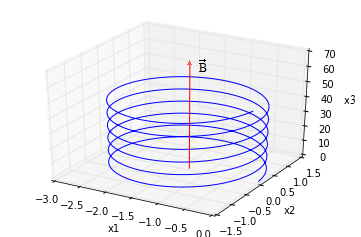
\includegraphics[width=0.5\linewidth]{img/figure_1}
  \captionof{figure}{\emph{Movimiento helicoidal de un electrón ($q=-e$) en presencia de un campo magnético.}}
  \label{fig:helicoidal}
\end{figure}








%%%%%%%%%%%%%%%%%%%%%%%%%%%%%%%%%%%%%%%%%%%%%
\subsection{\texorpdfstring{Movimiento en el plano: $\mathbb{R}^2$ }%
                               {Movimiento en el plano}}
$$\\$$%%%%%%%%%%%%%%%%%%%%%%%%%%%%%%%%%%%%%%%%%%%%%










Si restringimos el movimiento al plano $X_1X_2$, el campo magnético, es perpendicular a la dirección del movimiento de la partícula en todo el plano, por lo que la solución se corresponde con (\ref{Solucion Lorentz}) eliminando la dimensión $x_3$. Si además estudiamos el movimiento desde dentro de este nuevo espacio, considerando este como un espacio bidimensional embebido en uno de dimensión superior donde $$\\$$
\begin{equation*}
\vec{E}=(E_1,E_2,E_3) \hspace{3cm} \vec{B}=(B_1,B_2,B_3) \qquad ,
\end{equation*} $$\\$$
los campos eléctrico y magnético pasan a tener la forma $$\\$$
\begin{equation}
\vec{E}=(E_1,E_2) \hspace{3cm} B=B_3 \qquad .
\end{equation} $$\\$$
El campo eléctrico pierde simplemente la tercera componente espacial (al igual que le ocurre al potencial vector $\vec{A}=(A_1,A_2)$). El campo magnético, en cambio, no ve reducida una de sus dimensiones, si no que pasa de entenderse, al ser un vector perpendicular al espacio, como un pseudo-escalar. Esto hace que no sea válida la expresión de los potenciales como los vimos en (\ref{potenciales y campos electromagneticos}), ya que no es posible construir un pseudo-escalar como un producto vectorial, no obstante, esto se puede corregir reescribiendo los campos como $$\\$$
\begin{equation}
\vec{E}= - \vec{\triangledown} \phi - \frac{\partial \vec{A}}{\partial t} \hspace{3cm} B = \partial_1 A_2 - \partial_2 A_1 \qquad . 
\end{equation} $$\\$$
El operador diferencia $\vec{\triangledown}$ en el plano se define $$\\$$
\begin{equation}
\vec{\triangledown}= \frac{\partial}{\partial x_1} \vec{e}_1 + \frac{\partial}{\partial x_2} \vec{e}_2 \qquad .
\end{equation} $$\\$$
Con esta nueva expresión de los campos se pueden restringir los resultados obtenidos en el espacio tridimensional al plano. 
%La estructura formal de los potenciales en un espacio tridimensional es idéntica a la del plano en el problema clásico, por lo que no es necesario hacer un formalismo específico para este problema. $$\\$$
La soluciones en este espacio para el movimiento de la partícula son por tanto $$\\$$
\begin{equation}
\begin{cases}
x_1=A \; {\rm cos} \left( \frac{q B}{m} t + \theta_0\right) + C'_1  \qquad \quad {}$$\\$$
x_2=A \; {\rm sen} \left( \frac{q B}{m} t + \theta_0\right) + C'_2   \qquad ,\end{cases}
\end{equation} $$\\$$
que es la misma que habíamos visto en (\ref{Solucion Lorentz}), sin la tercera componente $x_3(t)=0$. Tanto en el caso tridimensional con movimiento perpendicular a $\vec{B}$, como en el plano, las partículas describen una trayectoria circular centrada en el punto $(C'_1,C'_2)$ con una velocidad de rotación $\omega_c$,  $$\\$$
\begin{equation} 
\omega_c = \frac{\vert q \vert B}{m} = \frac{eB}{m} \qquad e>0 \qquad ,
\end{equation} $$\\$$
denominada frecuencia de ciclotrón. Una vez fijado el sentido del vector del campo magnético como el sentido positivo en el eje $x_3$, el sentido de rotación de las partículas depende del signo de la carga eléctrica, siendo positivo para partículas con carga $q=-e$ (como los electrones) y negativo para partículas con $q=e$ donde $e>0$. $$\\$$
\begin{figure}
\centering
\begin{minipage}{.5\textwidth}
  \centering
  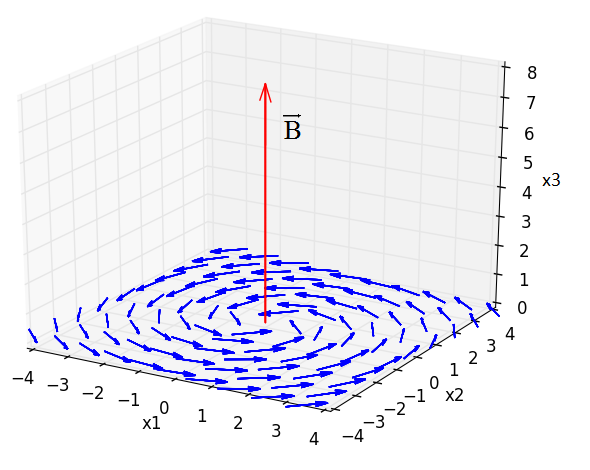
\includegraphics[width=1\linewidth]{img/figure_2}
  \captionof{figure}{\emph{Sentido de giro para} $q=-e \; , \; e>0$ }
  \label{fig:test1}
\end{minipage}%
\begin{minipage}{.5\textwidth}
  \centering
  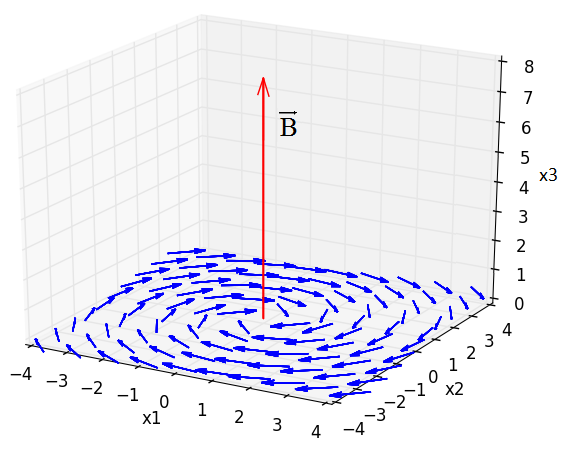
\includegraphics[width=1\linewidth]{img/figure_3}
  \captionof{figure}{\emph{Sentido de giro para} $q=e \;, \; e<0$}
  \label{fig:test2}
\end{minipage}
\end{figure}








\newpage
\leavevmode\thispagestyle{empty}\newpage


$$\\$$%%%%%%%%%%%%%%%%%%%%%%%%%%%%%%%%%%%%%%%%%%%%%
\section{El problema cuántico de Landau}
$$\\$$%%%%%%%%%%%%%%%%%%%%%%%%%%%%%%%%%%%%%%%%%%%%%










En la sección anterior hemos obtenido la trayectoria clásica de una partícula cargada que se mueve en un campo magnético uniforme. En este apartado estudiaremos el problema cuántico correspondiente. Llevaremos a cabo la cuantización canónica del sistema considerado, de modo que la posición y el momento de la partícula pasan de ser magnitudes clásicas a ser operadores de la teoría siguiendo la representación de Schroedinger [6]. $$\\$$
\begin{equation} \label{estados propios}
{x_i,p_i} \hspace{2cm} \longrightarrow \hspace{2cm} {\hat{x}_i, \hat{p}_i} \qquad , \qquad i =1,2,3. \qquad .
\end{equation} $$\\$$
Se denomina cuantización canónica a considerar las relaciones de conmutación $$\\$$
\begin{equation}
[\hat{x_i},\hat{p_j}] = i \hbar \delta_{ij} \hspace{1.5cm},\hspace{1.5cm} [\hat{x_i},\hat{x_j}]=[\hat{p_i},\hat{p_j}]=0 \qquad .
\end{equation} $$\\$$
de modo que se definen los operadores momento y energía como $$\\$$
\begin{equation}
\hat{p}_i = - i \hbar \frac{\partial}{\partial x_i} \hspace{3cm} \hat{E} = i \hbar \frac{\partial}{\partial t} \qquad,
\end{equation} $$\\$$
%Podemos obtener la función de onda, $\psi$, que describe a la partícula por medio de la función hamiltoniana en términos de operadores cuánticos. Esta función se corresponde con la expresión clásica, sustituyendo las magnitudes clásicas por operadores cuánticos. Para el Hamiltoniano de  partícula libre tenemos que
El Hamiltoniano de partícula libre es $$\\$$
\begin{equation}
\hat{H}\psi(\vec{x},t) = \frac{1}{2m} \hat{p}_i \hat{p}_i \psi(\vec{x},t) = \hat{E} \psi(\vec{x},t) \qquad \rightarrow \qquad - \frac{\hbar^2}{2m} \frac{\partial^2 \psi (\vec{x},t)}{\partial x_i \partial x_i} = i \hbar \frac{\partial}{\partial t} \psi (\vec{x},t) \qquad . 
\end{equation} $$\\$$
Esta es la ecuación de Schroedinger dependiente del tiempo para la partícula libre. En el caso de que el problema sea independiente del tiempo, esta ecuación se puede reducir a un problema de autovalores para la energía: $$\\$$
\begin{equation}
\hat{H} \psi (\vec{x}) = E \psi(\vec{x})  \qquad \Rightarrow \qquad \psi(\vec{x},t) = \psi(\vec{x})e^{i \frac{Et}{\hbar}}\qquad .
\end{equation} $$\\$$








$$\\$$%%%%%%%%%%%%%%%%%%%%%%%%%%%%%%%%%%%%%%%%%%%%%
\subsection{\texorpdfstring{Espectro y funciones de onda en $\mathbb{R}^3$}%
                               {Espectro y funciones de onda en el espacio}}
$$\\$$%%%%%%%%%%%%%%%%%%%%%%%%%%%%%%%%%%%%%%%%%%%%%








Este problema consiste en el cálculo de los estados propios y autovalores del Hamiltoniano que describe una partícula cargada en presencia de un campo magnético uniforme. Se tomará este en la dirección $\vec{e}_3$. El Hamiltoniano de este problema es análogo al que habíamos visto para el problema clásico en (\ref{Lorentz Hamilton}), sustituyendo las variables canónicas por operadores, y eliminando el término de potencial escalar al no tener campo eléctrico, resulta: $$\\$$
\begin{equation} \label{Schroedinger campo magnetico}
\hat{H} = \frac{1}{2m} (\hat{p}_i + \frac{e}{c} A_i) (\hat{p}_i + \frac{e}{c} A_i) \qquad .
\end{equation} $$\\$$
Se ha sustituido el valor de la carga por $q=-e$ para referirnos concretamente a electrones. Además hemos pasado de utilizar las unidades cgs, a las unidades racionalizadas de Lorentz-Heaviside introduciendo el factor $c^{-1}$ en la carga (por conveniencia en apartados posteriores). Con estas condiciones, escogemos el gauge de Landau [4] para el potencial vector $$\\$$
\begin{equation} \label{gauge de landau}
\vec{A} = (-B x_2,0,0) \qquad ,
\end{equation} $$\\$$
de modo que la ecuación de autovalores es $$\\$$
\begin{equation} \label{Hamiltoniano Landau 3D}
\frac{1}{2m} \left[(\hat{p}_1 - \frac{e}{c}B x_2)^2 + \hat{p}_2^2 + \hat{p}_3^2 \right] \psi(\vec{x}) = E \psi(\vec{x}) \qquad .
\end{equation}$$\\$$
Esta ecuación no depende de las coordenadas $x_1$ y $x_3$, por lo que podemos buscar soluciones de la forma $$\\$$
\begin{equation}
\psi(\vec{x}) = exp \left\lbrace \frac{i}{\hbar} (p_1 x_1 + p_3 x_3)\right\rbrace \chi(x_2) \qquad ,
\end{equation} $$\\$$
que es propia de $\hat{p}_1$ y $\hat{p}_3$ con autovalores $p_1$ y $p_3$, respectivamente. De modo que sustituyendo en la ecuación obtenemos $$\\$$
\begin{equation*}
\frac{1}{2m} \left[ (p_1 - \frac{e}{c}B x_2)^2 + \hat{p_2}^2 + p_3^2\right] \chi (x_2) = E \chi(x_2) \qquad.
\end{equation*} $$\\$$
Es importante notar que ahora las magnitudes $p_1$ y $p_3$ ya no son operadores, sino que son los autovalores correspondientes. Esta ecuación se puede reescribir como $$\\$$
\begin{equation*}
\left[ -\frac{\hbar^2}{2m} \frac{\partial}{\partial x_2^2} + \frac{1}{2}\frac{e^2B^2}{mc^2}\left( x_2 - \frac{p_1c}{eB}\right)^2 \right] \chi(x_2) = \left(E - \frac{p_3^2}{2m}\right)\chi(x_2) \qquad .
\end{equation*} $$\\$$
El miembro de la izquierda se corresponde con el Hamiltoniano de un oscilador armónico simple de frecuencia $\omega_c = eB/mc$ y centrado en $+p_1c/eB$. Este es el mismo resultado que obtuvimos para una partícula clásica, lo cual era de esperar, la diferencia está, como vamos a ver, en los posibles valores energéticos. Los autovalores de este Hamiltoniano son: $$\\$$
\begin{equation}
 \hat{H}_{osc} \phi_{osc} = E_{n} \phi_{osc} \hspace{4cm} E_{n}= \hbar \omega_c \left( n + \frac{1}{2} \right) \qquad ,
\end{equation} $$\\$$
donde n=0,1,2,3,...$\infty$. Además, sabemos que los estados propios, $\phi$, tienen la forma  $$\\$$
\begin{equation} \label{autoestados oscilador} 
\chi_n(x_2) = \frac{1}{\pi^{\frac{1}{4}} l_c^{\frac{1}{2}} (2^n n!)^{\frac{1}{2}}} exp \left\lbrace - \frac{(x_2 - C'_2)}{l_c}\right\rbrace H_n \left( \frac{x_2 - C'_2}{l_c} \right) \hspace{1cm} , \hspace{1cm} l_c^2 \equiv \left( \frac{\hbar}{m \omega_c} \right) \qquad.
\end{equation} $$\\$$
El coeficiente, $C'_2=p_1c/qB$, se corresponde, con el centro del oscilador. En la expresión anterior hemos definido la longitud magnética, $l_c$, y además hemos introducido los polinomios de hermite de grado n, $H_n(x)$. De modo que a partir de los niveles energéticos del Hamiltoniano del oscilador podemos obtener la energía de una partícula cuántica cargada en presencia de un campo magnético de la forma $\vec{B}=B \vec{e}_3$: $$\\$$
\begin{equation}
\hat{H}_{osc} \chi(x_2) = \left( E - \frac{p_3^2}{2m} \right) \chi (x_2) \hspace{3cm} \longrightarrow \hspace{3cm} E_{osc} = \left( E - \frac{p_3^2}{2m} \right) $$\\$$
E= \hbar \omega_c \left( n + \frac{1}{2}\right) + \frac{p_3^2}{2m} \qquad .
\end{equation} $$\\$$
La energía, por tanto, depende del momento en la dirección paralela al campo (el cual no se ve afectado por este) y de la energía de oscilación de la partícula en el plano perpendicular al campo. Fijando el valor del momento $p_3$, los niveles de energía son discretos. Por otro lado, los autoestados del Hamiltoniano son $$\\$$
\begin{equation}
\psi_{p_1,p_3,n}=exp \left\lbrace \frac{i}{\hbar} (p_1 x_1 + p_3 x_3) \right\rbrace \frac{1}{\pi^{\frac{1}{4}} l_c^{\frac{1}{2}} (2^n n!)^{\frac{1}{2}}} exp \left\lbrace - \frac{1}{l_2}(x_2 - \frac{p_1c}{eB})\right\rbrace H_n \left( \frac{x_2 - C'_2}{l_c} \right)  \qquad.
\end{equation} $$\\$$
Estos estados vienen caracterizados por los números cuánticos ${p_1,p_3,n}$. La elección de esos número cuánticos no es la única elección posible para construir una base de estados propios del sistema para este problema, si no que viene determinada por la elección de gauge que hemos hecho para el potencial vector (gauge de Landau). En el caso de escoger otro gauge podríamos obtener una base de estados propios en función de otros números cuánticos (como por ejemplo en el gauge simétrico, como veremos a continuación), no obstante, el comportamiento físico de las partículas en presencia de un campo magnético es independiente de la elección de gauge, como ya dijimos. $$\\$$ 
El hecho de que hayamos construido una base de estados propios en función del número cuántico $p_1$ y que la energía no dependa de este, hace que exista una degeneración en $p_1\in (-\infty, \infty)$ de los niveles energéticos, además, al ser posible cualquier valor de $p_1$ en cada nivel energético la degeneración en cada uno  de estos es infinita. Esta degeneración infinita se convierte en finita si limitamos el espacio a un volumen finito y establecemos unas condiciones de contorno periódicas. Si, en el plano prependicular a $\vec{B}$, restringimos la oscilación a un cuadrado de dimensiones $L_1$ y $L_2$, resulta $$\\$$
\begin{equation*}
e^{-\frac{i}{\hbar}p_1 L_1} = 1 \hspace{2cm} \longrightarrow \hspace{2cm} p_1 = \frac{2 \pi \hbar m}{L_1} \hspace{ 3cm} m \in \mathbb{Z} \qquad .
\end{equation*} $$\\$$
Por lo tanto los valores de $p_1$ dejan de estar en el continuo. Como vimos, el centro de oscilación, $C'_2$, depende de $p_1$, con lo que el centro también deja de tener cualquier valor posible y pasa a tener valores discretos $$\\$$
\begin{equation*}
\Delta p_1 = \frac{2 \pi \hbar}{L_1} \hspace{1.5cm},\hspace{1.5cm} \Delta C'_1 = \frac{2 \pi \hbar c}{e B L_1} \equiv  \frac{h c}{e B L_1} \qquad.
\end{equation*} $$\\$$
De modo que el número de posibles valores para $p_1$ es el mismo que el número de posibles centros de oscilación en la dimensión $x_2$ dentro del volumen que hemos definido. Esto nos da el número de estados por nivel energético, que viene dado por $$\\$$
\begin{equation}
n^{\circ} \quad de \quad estados = \frac{L_2}{\Delta C'_2} = \frac{L_1 L_2}{2 \pi \hbar c} e B \equiv  \frac{L_1 L_2}{h c} e B \qquad . 
\end{equation} $$\\$$
Del mismo modo podemos ver que las dimensiones del cuadrado a las que tenemos que restringir la oscilación, para que los niveles no estén degenerados, es: $$\\$$
\begin{equation*}
L_1 L_2 = \frac{2 \pi \hbar c}{e B} \equiv \frac{h c}{e B} \qquad .
\end{equation*} $$\\$$
Si además las partículas están restringidas en la dirección $\vec{e}_3$, los posibles valores de $p_3$ dejan de ser continuos y pasan a ser discretos, y con ello también los posibles niveles energéticos. $$\\$$
\begin{equation}
p_3 = \frac{2 \pi \hbar k}{L_3}\hspace{ 3cm} k \in \mathbb{Z} \qquad
\end{equation} $$\\$$
De esta forma caracterizamos todos los estados por medio de los números cuánticos $n$, $k$ y $m$. La energía del sistema viene caracterizada por los númeroscuánticos $n$ y $k$, mientras que $m$ caracteriza la degeneración para cada nivel de energía.  $$\\$$
\begin{equation}
E= \hbar \omega_c \left( n + \frac{1}{2}\right) + \frac{h^2 k^2}{2m L_3^2} \qquad .
\end{equation} $$\\$$
En función de estos números cuánticos, la función de onda completa se escribe como $$\\$$
\begin{equation}
\psi_{n,k,m}(\vec{x})=exp \left\lbrace i (\frac{2 \pi m}{L_1} x_1 + \frac{2 \pi k}{L_3} x_3) \right\rbrace \frac{1}{\pi^{\frac{1}{4}} l_c^{\frac{1}{2}} (2^n n!)^{\frac{1}{2}}} exp \left\lbrace - \frac{1}{l_c}\left(x_2 - \frac{cp_1}{eB}\right)\right\rbrace H_n \left( \frac{x_2 - C'_2}{l_c} \right)  \qquad.
\end{equation} $$\\$$

\begin{figure}
  \centering
  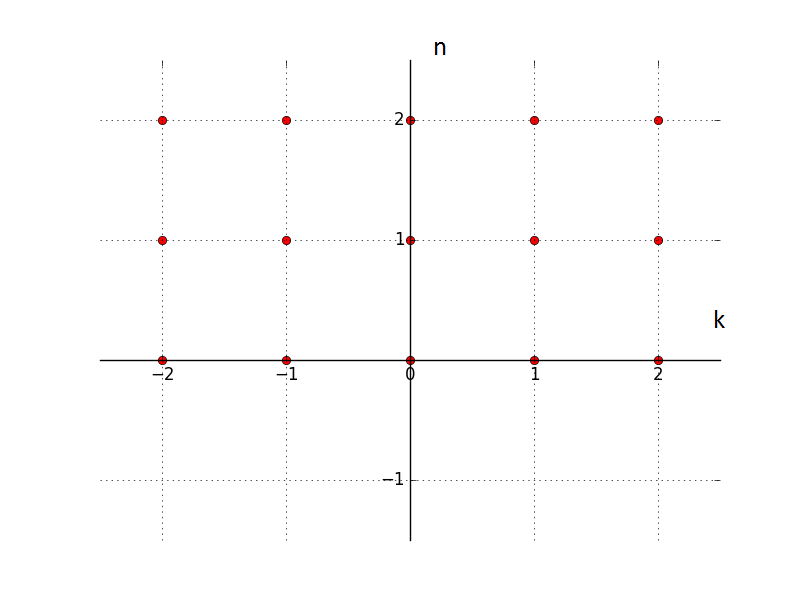
\includegraphics[width=0.5\linewidth]{img/figure_4}
  \captionof{figure}{\emph{Estados no degenerados de Landau en el gauge de Landau en función de n y k.}}
  \label{fig:gauge landau}
\end{figure}









$$\\$$%%%%%%%%%%%%%%%%%%%%%%%%%%%%%%%%%%%%%%%%%%%%%
\subsection{\texorpdfstring{Espectro y funciones de onda en $\mathbb{R}^2$}%
                               {Espectro y funciones de onda en el plano}}
$$\\$$%%%%%%%%%%%%%%%%%%%%%%%%%%%%%%%%%%%%%%%%%%%%%










La restricción al plano, como vimos, la hacemos eliminando la tercera componente espacial de modo que ahora la ecuación (\ref{Hamiltoniano Landau 3D}) se escribe como $$\\$$
\begin{equation}
\frac{1}{2m} \left[ (\hat{p}_1 -\frac{e}{c}x_2B)^2 + \hat{p}_2^2\right] \psi = E \psi \qquad.
\end{equation} $$\\$$
Al no depender de $x_1$, proponemos una solución de onda plana para $\psi(\vec{x})$ en esa dirección $$\\$$
\begin{equation}
\psi (\vec{x}) = exp \left\lbrace \frac{i}{\hbar} p_1 x_1\right\rbrace \chi(x_2) \qquad . 
\end{equation} $$\\$$
Sustituyendo en la ecuación de Schroedinger nos queda $$\\$$
\begin{equation*}
\left[ - \frac{\hbar^2}{2m} \frac{\partial^2}{\partial_2^2} + \frac{1}{2} \frac{e^2 B^2}{mc^2} \left( x_2 - \frac{cp_1}{eB}\right)^2\right]\chi(x_2)= E \chi (x_2) \qquad .
\end{equation*} $$\\$$
\begin{figure}
  \centering
  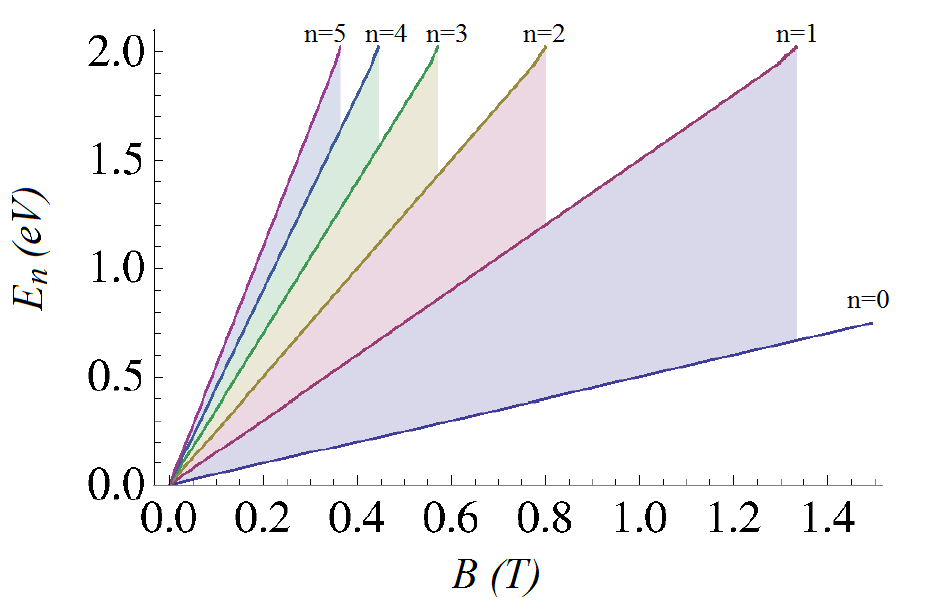
\includegraphics[width=0.5\linewidth]{img/figure_6}
  \captionof{figure}{\emph{Abanico de Landau. Representación de los posibles valores de energía de los electrones, en el problema de Landau en el plano, según el valor del campo magnético }[11].} \label{fig:Abanico clasico}
\end{figure}
Como antes, el término de la izquierda se corresponde con el Hamiltoniano de un oscilador armónico simple con los mismos valores de frecuencia y centro de oscilación, por lo tanto, la función $\chi(x_2)$ viene dada, también en este caso, por los autoestados de oscilador (\ref{autoestados oscilador}). La diferencia está en el término de la derecha, en el que ahora no aparece el término cinético asociado a la dirección $\vec{e}_3$, de modo que los niveles energéticos en este caso son $$\\$$
\begin{equation} \label{energia oscilador}
E = E_{osc}=\hbar \omega_c \left( n + \frac{1}{2} \right) \qquad ,
\end{equation} $$\\$$
donde $\omega_c$ sigue siendo la frecuencia ciclotrón: $$\\$$
\begin{equation}
\omega_c = \frac{eB}{mc}
\end{equation} $$\\$$
En el problema en el espacio los niveles energéticos tenían un término en el continuo, debido al término cinético en la dirección del campo, pero que se podía discretizar si nos restringíamos a un espacio de volumen finito. En este caso son directamente discretos al depender solo de la energía de oscilación. Esta energía solo depende de la intensidad del campo magnético, $B$, como vemos en la Figura \ref{fig:Abanico clasico}. $$\\$$
Los autoestados ahora, vienen determinados solo por dos números cuánticos $p_1$ y $n$. Debido a que la energía es independiente de $p_1$, tenemos una degeneración infinita y continua en $p_1$ que, como antes, podemos convertir en infinita pero numerable si limitamos el espacio a un cuadrado de dimensiones $L_1$ y $L_2$, de modo que obtenemos el mismo número de estados por cada nivel de energía que en $\mathbb{R}^3$. $$\\$$
\begin{equation}
p_1 = \frac{2 \pi \hbar m}{L_1} \equiv \frac{h m}{L_1} \hspace{ 3cm} m \in \mathbb{Z} \qquad ,
\end{equation} $$\\$$
y el número de estados por nivel energético es:$$\\$$
\begin{equation*}
n^\circ \quad de \quad estados = \frac{L_1 L_2}{2 \pi \hbar c} e B \equiv \frac{L_1 L_2}{h c} e B \qquad . 
\end{equation*} $$\\$$
En función de los números cuánticos $n$ y $m$ la función de onda propia del Hamiltoniano es: $$\\$$
\begin{equation}
\psi_{n,m} (\vec{x}) = exp \left\lbrace  \frac{i h m}{L_1} x_1\right\rbrace \frac{1}{\pi^{\frac{1}{4}} l_c^{\frac{1}{2}} (2^n n!)^{\frac{1}{2}}} exp \left\lbrace - \frac{1}{l_c}\left(x_2 - \frac{cp_1}{eB}\right)\right\rbrace H_n \left( \frac{x_2 - C'_2}{l_c} \right) \hspace{1cm} \qquad . 
\end{equation} $$\\$$
Concluyendo, vemos que la restricción al plano del problema de Landau supone una reducción de los grados de libertad que nos disminuye el número de números cuánticos necesarios para caracterizar una base de autoestados del problema. Aparte de eso, el problema es completamente análogo al caso tridimensional. $$\\$$









$$\\$$%%%%%%%%%%%%%%%%%%%%%%%%%%%%%%%%%%%%%%%%%%%%%%%%
\subsection{\texorpdfstring{Espectro y funciones de onda en $\mathbb{R}^2$ con gauge simétrico}%
                               {Espectro y funciones de onda en el plano con gauge simétrico}}
$$\\$$%%%%%%%%%%%%%%%%%%%%%%%%%%%%%%%%%%%%%%%%%%%%%%%%%









En la sección anterior hemos estudiado el problema de una partícula cargada en presencia de un campo magnético constante usando el gauge de Landau. La invarianza gauge de los potenciales electromagnéticos nos dice que el comportamiento de las partículas debe ser independiente del gauge elegido, pero la solución a la ecuación (\ref{Schroedinger campo magnetico}) puede ser diferente, y de hecho lo es. $$\\$$
De manera análoga a como definimos el gauge simétrico en el espacio (\ref{gauges}), en el plano [29] consideramos:  $$\\$$
\begin{equation} \label{gauge simetrico}
A_{s}=(-\frac{B}{2} x_2,\frac{B}{2} x_1) \qquad ,
\end{equation} $$\\$$
con el cual el Hamiltoniano del sistema (\ref{Schroedinger campo magnetico}) es ahora: $$\\$$
\begin{equation} \label{h gauge simetrico}
\hat{H}= \frac{1}{2m}\left[\left( - i \hbar \frac{\partial}{\partial x_1} - \frac{eB}{2c} x_2 \right)^2 + \left( -i \hbar \frac{\partial}{\partial x_2} + \frac{eB}{2c} x_1\right)^2 \right] = $$\\$$
 = \frac{1}{2m} \left[ -\hbar^2 \left(\frac{\partial^2}{\partial x_1^2} + \frac{\partial^2}{\partial x_2^2}\right) + \frac{e^2B^2}{4c^2}\left( x_1^2 + x_2^2\right) + i\hbar \frac{eB}{c} \left( x_2 \frac{\partial}{\partial x_1} - x_1 \frac{\partial}{\partial x_2} \right)\right]\qquad .
\end{equation} $$\\$$
El último término de la expresión anterior podemos reescribirlo en función del momento angular: $$\\$$
\begin{equation}
L_k = \epsilon_{ijk}x_i p_j \hspace{1.5cm},\hspace{1.5cm} L_3 = x_1p_2 - x_2p_1 \qquad .
\end{equation} $$\\$$
Entonces, el Hamiltoniano se puede escribir como $$\\$$
\begin{equation} \label{gauge simetrico L3}
\hat{H} = \frac{1}{2m} \left[ -\hbar^2 \left(\frac{\partial^2}{\partial x_1^2} + \frac{\partial^2}{\partial x_2^2}\right) + \frac{e^2B^2}{4c^2}\left( x_1^2 + x_2^2\right) - i\hbar \frac{eB}{c} L_3 \right] \qquad .
\end{equation} $$\\$$
Para resolver esta ecuación introducimos los siguientes operadores: $$\\$$
\begin{equation} 
\hat{a} = \frac{1}{\sqrt{2}} \left[ \left( \frac{x_1}{2 l_c} + l_c \frac{\partial}{\partial x_1} \right) - i \left( \frac{x_2}{2 l_c} + l_c \frac{\partial}{\partial x_2}\right) \right] \qquad , \qquad
\hat{a}^\dagger = \frac{1}{\sqrt{2}} \left[ \left( \frac{x_1}{2 l_c} - l_c \frac{\partial}{\partial x_1} \right) + i \left( \frac{x_2}{2 l_c} - l_c \frac{\partial}{\partial x_2}\right) \right] \qquad {} $$\\$$
\hat{b} = \frac{1}{\sqrt{2}} \left[ \left( \frac{x_1}{2 l_c} + l_c \frac{\partial}{\partial x_1} \right) + i \left( \frac{x_2}{2 l_c} + l_c \frac{\partial}{\partial x_2}\right) \right] \qquad,\qquad
\hat{b}^\dagger = \frac{1}{\sqrt{2}} \left[ \left( \frac{x_1}{2 l_c} - l_c \frac{\partial}{\partial x_1} \right) - i \left( \frac{x_2}{2 l_c} - l_c \frac{\partial}{\partial x_2}\right) \right] \qquad ,
\end{equation} $$\\$$
tales que los únicos conmutadores no nulos son $$\\$$
\begin{equation*}
[ \hat{a}, \hat{a}^\dagger]=[ \hat{b},\hat{b}^\dagger]= 1 \qquad .
\end{equation*} $$\\$$
En términos de estos operadores podemos escribir el Hamiltoniano como $$\\$$
\begin{equation}
\hat{H} = \hbar \omega_c \left( \hat{a}^\dagger \hat{a} + \frac{1}{2}\right) = \hbar \omega_c \left( \hat{N} + \frac{1}{2}\right) \qquad  \hspace{3cm} n=0,1,2,3,... \qquad ,
\end{equation} $$\\$$
donde se define $\hat{N}=\hat{a}^\dagger\hat{a}$ como el operador número, tal que $$\\$$
\begin{equation*}
\hat{a}^\dagger \hat{a}\psi=\hat{N} \psi = n\psi \qquad.
\end{equation*} $$\\$$
%El término $\hat{a}^\dagger \hat{a}$ constituye la expresión del Hamiltoniano (\ref{h gauge simetrico}), mientras que el término 1/2, lo hemos añadido libremente, dado que la función hamiltoniana está definida salvo constante aditiva. %chapuza
De modo que los niveles energéticos vienen dados por $$\\$$
\begin{equation}
E_n = \hbar \omega_c \left( n + \frac{1}{2}\right) \qquad {} 
\end{equation} $$\\$$
Esta expresión es la misma que hemos obtenido en el gauge de Landau (\ref{energia oscilador}). Esto se debe a que la estructura de los niveles energéticos es independiente de la elección de gauge. $$\\$$
Del mismo modo podemos escribir la tercera componente del momento angular en función de los operadores $\hat{a}$, $\hat{a}^\dagger$, $\hat{b}$ y $\hat{b}^\dagger$ $$\\$$
\begin{equation*}
\hat{L}_3 = \hbar(\hat{b}^\dagger \hat{b} - \hat{a}^\dagger \hat{a}) \qquad .
\end{equation*} $$\\$$
Teniendo en cuenta las relaciones de conmutación de $\hat{a}$, $\hat{a}^\dagger$, $\hat{b}$ y $\hat{b}^\dagger$ vemos que $[\hat{H}, \hat{L}_3]=0$, por lo que podemos buscar una base de estados propios comunes a ambos  operadores $\hat{H}$ y $\hat{L}_3$  $$\\$$
\begin{equation}
\hat{H}\psi_{n,m} = \hbar \omega_c \left(n + \frac{1}{2} \right) \psi_{n,m} \hspace{3cm} \hat{L_3}\psi_{n,m} = \hbar m \psi_{n,m} \qquad .
\end{equation}$$\\$$
Para obtener el espectro de funciones de onda es conveniente escribir el problema en la notación de Dirac de brakets, donde los autoestados con números cuánticos n y m se escriben como $\ket{n,m}$, de modo que $$\\$$
\begin{equation}\label{operadorN}
\hat{N} = \hat{a}^\dagger \hat{a} \hspace{1.5cm},\hspace{1.5cm} \hat{L} = \hat{b}^\dagger \hat{b} - \hat{a}^\dagger \hat{a} $$\\$$
\hat{N} \ket{n,m}=n \ket {n,m} $$\\$$
\hat{L} \ket{n,m}=m \ket{n,m}
\end{equation} $$\\$$
En esta base, los operadores escalera actúan $$\\$$
\begin{equation} \label{actuacion escalera}
\hat{a}\ket{n,m}=\sqrt{n}\ket{n-1,m+1}  \hspace{1.5cm}, \hspace{1.5cm}
\hat{a}^\dagger \ket{n,m} = \sqrt{n+1} \ket{n+1,m-1}\qquad \qquad{} $$\\$$
\hat{b} \ket{n,m} = \sqrt{m+n} \ket{n,m-1} \hspace{1.5cm} , \hspace{1.5cm}
\hat{b}^\dagger \ket{n,m} = \sqrt{m+n+1} \ket{n,m+1} \qquad .
\end{equation} $$\\$$
Teniendo en cuenta la expresión (\ref{gauge simetrico L3}), los dos primeros sumandos constituyen dos Hamiltonianos de oscilador armónico en las direcciones $x_1$ y $x_2$, y por lo tanto, se cumple que la siguiente relación entre n y m $$\\$$
\begin{equation*}
n \geq - m \qquad ,
\end{equation*} $$\\$$
los estados en este problema aunque son autoestados de $L_3$, no lo son de $L^2$, por lo que la única restricción para el conjunto de posibles valores de m viene dada por la expresión anterior, que se puede escribir como $$\\$$
\begin{equation*}
-n \leq m < \infty  \hspace{3cm} m \in Z.
\end{equation*} $$\\$$
El estado que tiene n=m=0 es aniquilado por $\hat{a}$, al no poder existir valores negativos para n, y por $\hat{b}$, debido a la condición anterior para m $$\\$$
\begin{equation*}
\hat{a}\ket{0,0}=0 \hspace{3cm} \hat{b}\ket{0,0}=0 \qquad .
\end{equation*} $$\\$$
Para resolver estas ecuaciones es conveniente expresar los operadores en representación de coordenadas y definir: $$\\$$
\begin{equation}
z=x_1+ix_2 \hspace{3cm} \frac{\partial}{\partial z} =\frac{1}{2} \left( \frac{\partial}{\partial x_1} - i \frac{\partial}{\partial x_2} \right) \qquad {}$$\\$$
\bar{z}=x_1 - i x_2 \hspace{3cm} \frac{\partial}{\partial \bar{z}} = \frac{1}{2} \left( \frac{\partial}{\partial x_1} + i \frac{\partial}{\partial x_2} \right) \qquad .
\end{equation} $$\\$$
En esta representación los operadores escalera son: $$\\$$
\begin{equation} \label{operadores escalera}
\hat{a} = \frac{1}{\sqrt{2}}\left(\frac{\bar{z}}{2l_c} + 2l_c \frac{\partial}{\partial z} \right) \hspace{2cm}, \hspace{2cm}
\hat{a}^\dagger = \frac{1}{\sqrt{2}}\left(\frac{z}{2l_c} - 2l_c\frac{\partial}{\partial \bar{z}}\right)$$\\$$ \qquad {}
\hat{b} = \frac{1}{\sqrt{2}}\left(\frac{z}{2l_c} + 2l_c\frac{\partial}{\partial \bar{z}}\right) \hspace{2cm},\hspace{2cm}
\hat{b} ^\dagger = \frac{1}{\sqrt{2}}\left(\frac{\bar{z}}{2l_c} - 2l_c \frac{\partial}{\partial z} \right) \quad ,
\end{equation} $$\\$$
de modo que el estado con $n=0$ y $m=0$ o fundamental viene dado por $$\\$$
\begin{equation*}
\left(\frac{\bar{z}}{2l_c} + 2l_c \frac{\partial}{\partial z} \right) \psi_{0,0}=0 \hspace{2cm} \left(\frac{z}{2l_c} + 2l_c\frac{\partial}{\partial \bar{z}}\right)\psi_{0,0}=0 \qquad .
\end{equation*} $$\\$$
El estado fundamental es, por tanto, $$\\$$
\begin{equation}
\psi_{00}(z,\bar{z})= \frac{1}{l_c \sqrt{2 \pi}} e^{-\frac{z \bar{z}}{4 l_c^2}} \qquad ,
\end{equation} $$\\$$
donde hemos impuesto la condición de normalización $$\\$$
\begin{equation*}
\int^\infty _{-\infty} \int ^\infty _{-\infty} \psi_{0,0}^*(x_1,x_2) \psi_{0,0}(x_1,x_2)dx_1dx_2= 1 \qquad .
\end{equation*} $$\\$$ %\int^\infty _{-\infty} \int ^\infty _{-\infty} \psi_{n,m} \psi_{n',m'}dx_1dx_2=\delta_{n,n'} \delta_{m,m'} \qquad .
Podemos obtener los estado de un nivel superior aplicando de manera sucesivalos operadores $\hat{a}^\dagger$ y $\hat{b}^\dagger$ de la forma: $$\\$$
\begin{equation*}
\ket{n,m}=\frac{(\hat{a}^\dagger)^n}{\sqrt{n!}} \frac{(\hat{b}^\dagger)^{n+m}}{\sqrt{(n+m)!}} \ket{0,0} \qquad .
\end{equation*} $$\\$$
A partir de esta ecuación algebraica, podemos obtener las funciones de onda de forma general $$\\$$
\begin{equation}
\psi_{n,m} (z,\bar{z}) = \bra{z,\bar{z}}\ket{n,m}=\bra{z,\bar{z}}\frac{(\hat{a}^\dagger)^n}{\sqrt{n!}} \frac{(\hat{b}^\dagger)^{n+m}}{\sqrt{(n+m)!}} \ket{0,0} \qquad .
\end{equation} $$\\$$
Empezamos buscando una expresión para los estados $\psi_{0,m}(z,\bar{z})$, para ello empezamos buscando las funciones una a una aplicando de manera sucesiva el operador $\hat{b}^\dagger$ desde el estado fundamental, $\psi_{0,0}(z,\bar{z})$ $$\\$$
\begin{equation*}
\psi_{0,1}(z,\bar{z}) = \frac{1}{\sqrt{2}}\left(\frac{\bar{z}}{2l_c} - 2l_c \frac{\partial}{\partial z} \right) \psi_{0,0} = \frac{1}{\sqrt{2}}  \left(\frac{\bar{z}}{l_c}\right)\psi_{0,0}(z,\bar{z}) \qquad {} $$\\$$
\psi_{0,2}(z,\bar{z}) =\frac{1}{\sqrt{2}} \frac{1}{\sqrt{2}}\left(\frac{\bar{z}}{2l_c} - 2l_c \frac{\partial}{\partial z} \right) \frac{1}{\sqrt{2}}  \left(\frac{\bar{z}}{l_c}\right)\psi_{0,0} = \frac{1}{\sqrt{2}}  \left(\frac{\bar{z}}{\sqrt{2} l_c}\right)^2 \psi_{0,0}(z,\bar{z}) $$\\$$
\psi_{0,3}(z,\bar{z}) =\frac{1}{\sqrt{6}} \frac{1}{\sqrt{2}}\left(\frac{\bar{z}}{2l_c} - 2l_c \frac{\partial}{\partial z} \right) \frac{1}{\sqrt{2}}  \left(\frac{\bar{z}}{\sqrt{2} l_c}\right)^2 \psi_{0,0} = \frac{1}{\sqrt{6}}  \left(\frac{\bar{z}}{\sqrt{2} l_c}\right)^3 \psi_{0,0}(z,\bar{z}) \qquad {} $$\\$$
.\quad .\quad . \hspace{11cm}
\end{equation*} $$\\$$
En general, para el primer nivel de Landau con $n=0$ tenemos: $$\\$$
\begin{equation*} 
\psi_{0,m}(z,\bar{z}) = \frac{1}{\sqrt{m!}} \left(\frac{\bar{z}}{\sqrt{2}l_c} \right)^m \psi_{0,0}(z,\bar{z}) = \frac{1}{\sqrt{m!}} \left(\frac{\bar{z}}{\sqrt{2}l_c} \right)^m \frac{1}{l_c \sqrt{2 \pi}} e^{-\frac{z \bar{z}}{4 l_c^2}}\qquad . 
\end{equation*} $$\\$$
Del mismo modo, por medio de la aplicación sucesiva del operador $\hat{a}^\dagger$ podemos obtener los estados de la forma $\psi_{n,-n}$ $$\\$$
\begin{equation*}
\psi_{1,-1}(z,\bar{z}) = \frac{1}{\sqrt{2}}\left(\frac{z}{2l_c} - 2l_c\frac{\partial}{\partial \bar{z}}\right) \psi_{0,0}(z,\bar{z}) = \frac{1}{\sqrt{2}}\frac{z}{l_c} \psi_{0,0}(z,\bar{z}) \qquad {} $$\\$$
\psi_{2,-2}(z,\bar{z}) = \frac{1}{\sqrt{2}}\frac{1}{\sqrt{2}}\left(\frac{z}{2l_c} - 2l_c\frac{\partial}{\partial \bar{z}}\right)\frac{1}{\sqrt{2}}\frac{z}{l_c} \psi_{0,0}(z,\bar{z}) = \frac{1}{\sqrt{2}}\left(\frac{z}{\sqrt{2}l_c}\right)^2 \psi_{0,0}(z,\bar{z}) \qquad {} $$\\$$
\psi_{3,-3}(z,\bar{z}) = \frac{1}{\sqrt{6}}\frac{1}{\sqrt{2}}\left(\frac{z}{2l_c} - 2l_c\frac{\partial}{\partial \bar{z}}\right) \frac{1}{\sqrt{2}}\left(\frac{z}{\sqrt{2}l_c}\right)^2 \psi_{0,0}(z,\bar{z}) = \frac{1}{\sqrt{6}}\left(\frac{z}{\sqrt{2}l_c}\right)^3 \psi_{0,0}(z,\bar{z}) \qquad  {} $$\\$$ . \quad . \quad . \hspace{11cm}
\end{equation*} $$\\$$
De forma que: $$\\$$
\begin{equation*} 
\psi_{n,-n}(z,\bar{z}) = \frac{1}{\sqrt{n!}} \left(\frac{z}{\sqrt{2}l_c} \right)^n \psi_{0,0}(z,\bar{z}) = \frac{1}{\sqrt{n!}} \left(\frac{z}{\sqrt{2}l_c} \right)^n \frac{1}{l_c \sqrt{2 \pi}} e^{-\frac{z \bar{z}}{4 l_c^2}} \qquad .
\end{equation*} $$\\$$
Finalmente, a partir de las expresiones obtenidas para $\psi_{0,m}(z,\bar{z})$ y $\psi_{n,-n}(z,\bar{z})$, supongamos que $\psi_{n,m}(z,\bar{z})$ es de la forma: $$\\$$
\begin{equation}  \label{funcion de onda laguerre generalizado}
\psi_{n,m} = \left(-1\right)^n \quad \frac{\bar{z}^m}{l_c^{m+1}} \quad \sqrt{\frac{n!}{\pi (n+m)!}} \quad f_{nm} \left(\frac{|z|^2}{2 l_c^2}\right) \quad e^{-\frac{|z|^2}{2l_c^2}} \qquad .
\end{equation} $$\\$$
El término $f_{nm}(x)$ es una función desconocida en términos de los números cuánticos n y m. Para los estado de $\psi_{n,-n}(z,\bar{z})$ buscamos la función de onda de los estados de m superior aplicando el operador $\hat{b}^\dagger$ sucesivamente, para obtener las funciones de onda de forma explícita y así intentar obtener por inducción $f_{n,m}(x)$. $$\\$$
Partimos del estado $\psi_{1,-1}(z,\bar{z})$ y buscamos estados $\psi_{1,m}(z,\bar{z})$ aplicándole $\hat{b}^\dagger$ $\lq \lq m+1$" veces $$\\$$
\begin{equation*}
\psi_{1,0}(z,\bar{z}) = \frac{1}{\sqrt{2}} \left(\frac{\bar{z}}{2 l_c} - 2 l_c \frac{\partial}{\partial z}\right)\frac{z}{\sqrt{2}l_c}\psi_{0,0}(z,\bar{z}) = \left( \frac{|z|^2}{2 l_c^2} - 1 \right)\psi_{0,0}(z,\bar{z}) \qquad {}$$\\$$
\psi_{1,1}(z,\bar{z}) = \frac{1}{\sqrt{2}} \frac{1}{\sqrt{2}} \left(\frac{\bar{z}}{2 l_c} - 2 l_c \frac{\partial}{\partial z}\right) \left( \frac{|z|^2}{2 l_c^2} - 1 \right)\psi_{0,0}(z,\bar{z}) = $$\\$$ = \frac{1}{\sqrt{2}} \left[\left(\frac{|z|}{\sqrt{2}l_c}\right)^2 - 2\right] \frac{\bar{z}}{\sqrt{2}l_c}\psi_{0,0}(z,\bar{z}) \qquad {}$$\\$$
\psi_{1,2}(z,\bar{z}) = \frac{1}{\sqrt{6}} \frac{1}{\sqrt{2}} \left(\frac{\bar{z}}{2 l_c} - 2 l_c \frac{\partial}{\partial z}\right)\frac{1}{\sqrt{2}} \left[\left(\frac{|z|}{\sqrt{2}l_c}\right)^2 - 2\right] \frac{\bar{z}}{\sqrt{2}l_c}\psi_{0,0}(z,\bar{z}) = $$\\$$ =  \frac{1}{\sqrt{6}} \left[\left(\frac{|z|}{\sqrt{2}l_c} \right)^2 - 3\right] \left(\frac{\bar{z}}{\sqrt{2}l_c}\right)^2 \psi_{0,0}(z,\bar{z}) \qquad {} $$\\$$ . \quad . \quad . \hspace{11cm}
\end{equation*} $$\\$$
Obtenemos el siguiente estado avanzando en $\hat{a}^\dagger$, $\psi_{2,-2}(z,\bar{z})$, y buscamos los estados $\psi_{1,m}(z,\bar{z})$ aplicando $\hat{b}^\dagger$ $\lq \lq m+2 "$ veces $$\\$$
\begin{equation*}
\psi_{2,-1}(z,\bar{z}) = \frac{1}{\sqrt{2}} \left(\frac{\bar{z}}{2 l_c} - 2 l_c \frac{\partial}{\partial z}\right)\left(\frac{z}{\sqrt{2}l_c}\right)^2\psi_{0,0}(z,\bar{z}) = \frac{1}{2}\left[\left( \frac{|z|}{\sqrt{2} l_c} \right)^4 - 2\left(\frac{|z|}{\sqrt{2}l_c}\right)^2\right]\psi_{0,0}(z,\bar{z}) \qquad {}$$\\$$
\psi_{2,0}(z,\bar{z}) = \frac{1}{\sqrt{2}} \frac{1}{\sqrt{2}} \left(\frac{\bar{z}}{2 l_c} - 2 l_c \frac{\partial}{\partial z}\right) \frac{1}{2}\left[\left( \frac{|z|}{\sqrt{2} l_c} \right)^4 - 2\left(\frac{|z|}{\sqrt{2}l_c}\right)^2\right]\psi_{0,0}(z,\bar{z}) = $$\\$$ =  \frac{1}{2}\left[\left( \frac{|z|}{\sqrt{2} l_c} \right)^4 - 4\left(\frac{|z|}{\sqrt{2}l_c}\right)^2 + 2\right]\psi_{0,0}(z,\bar{z}) \qquad {}$$\\$$
\psi_{2,1}(z,\bar{z}) = \frac{1}{\sqrt{3}} \frac{1}{\sqrt{2}} \left(\frac{\bar{z}}{2 l_c} - 2 l_c \frac{\partial}{\partial z}\right) \frac{1}{2}\left[\left( \frac{|z|}{\sqrt{2} l_c} \right)^4 - 4\left(\frac{|z|}{\sqrt{2}l_c}\right)^2 + 2\right]\psi_{0,0}(z,\bar{z}) =  $$\\$$ = \frac{1}{2\sqrt{3}}\left[\left( \frac{|z|}{\sqrt{2} l_c} \right)^4 - 6\left(\frac{|z|}{\sqrt{2}l_c}\right)^2 + 6\right] \left(\frac{\bar{z}}{\sqrt{2}l_c}\right)\psi_{0,0}(z,\bar{z}) \qquad {} $$\\$$ . \quad . \quad . \hspace{11cm}
\end{equation*} $$\\$$
Comparando las expresiones sucesivas que obtenemos para las funciones de onda con la expresión (\ref{funcion de onda laguerre generalizado}), podemos ver que el término $f_{n,m}(x)$ se corresponde con los polinomios de Laguerre generalizados, ${L_n}^m(x)$, que vienen dados como solución a la ecuación: $$\\$$
\begin{equation}
x \frac{d ^2}{d x^2}{L_n}^m (x) + (m+1-x)\frac{d}{dx}{L_n}^m(x) + n{L_n}^m(x)=0 \qquad , 
\end{equation} $$\\$$
siendo las primeras soluciones $$\\$$
\begin{equation*}
{L_0}^m(x) = 1 \qquad{} $$\\$$ 
{L_1}^m(x) = -x + m + 1 \qquad{} $$\\$$
{L_2}^m(x) = \frac{1}{2}[x^2 - 2(m+2)x + (m+1)(m+2)] \qquad.
\end{equation*} $$\\$$
La expresión para las autofunciones de la ecuación de Schroedinger para una partícula cargada en un campo magnético uniforme, en el plano, y en el guage simétrico, es: $$\\$$
\begin{equation} \label{autoestados simetricos}
\psi_{n,m}(z,\bar{z}) = \left(-1\right)^n \quad \frac{\bar{z}^m}{l_c^{m+1}} \quad \sqrt{\frac{n!}{\pi (n+m)!}} \quad {L_n}^m \left(\frac{|z|^2}{2 l_c^2}\right) \quad e^{-\frac{|z|^2}{2l_c^2}} \qquad .
\end{equation} $$\\$$
de forma que cumplen la condición de ortonormalidad $$\\$$
\begin{equation}
\int^\infty _{-\infty} \int ^\infty _{-\infty} \psi_{n,m}^* (x_1,x_2) \psi_{n',m'}(x_1,x_2)dx_1dx_2=\delta_{n,n'} \delta_{m,m'} \qquad .
\end{equation} $$\\$$ $$\\$$
Comparando las dos representaciones de manera general vemos que aunque la estructura de los niveles energéticos (así como el hecho de que estén degenerados) es independiente de la elección de gauge que hagamos para el potencial, lo que sí que depende del gauge son los números cuánticos con los que construimos la base de autoestados ($n$ y $p_3$ en el gauge de Landau y $n$ y $m$ en el gauge simétrico), lo cual es debido a las simetrías adicionales que aporta el gauge, más allá de las que ya tenga el problema. En la expresión del gauge de Landau (\ref{gauge de landau}) vemos que es invariante bajo traslaciones en la dirección $\vec{e}_1$, por lo que las funciones de onda que obtenemos a través de este son autoestados de $\hat{p}_1$, del mismo modo, el gauge simétrico (\ref{gauge simetrico}) es invariante bajo rotaciones en el plano $X_1X_2$, por lo que en este caso, las funciones de onda son autoestados del momento angular en la dirección perpendicular al plano, $\hat{L}_3$. $$\\$$
%A pesar de que en una teoría más realista es necesario tener en cuenta la interacción del espín de las partículas con el campo magnético, este estudio 
\begin{figure}
  \centering
  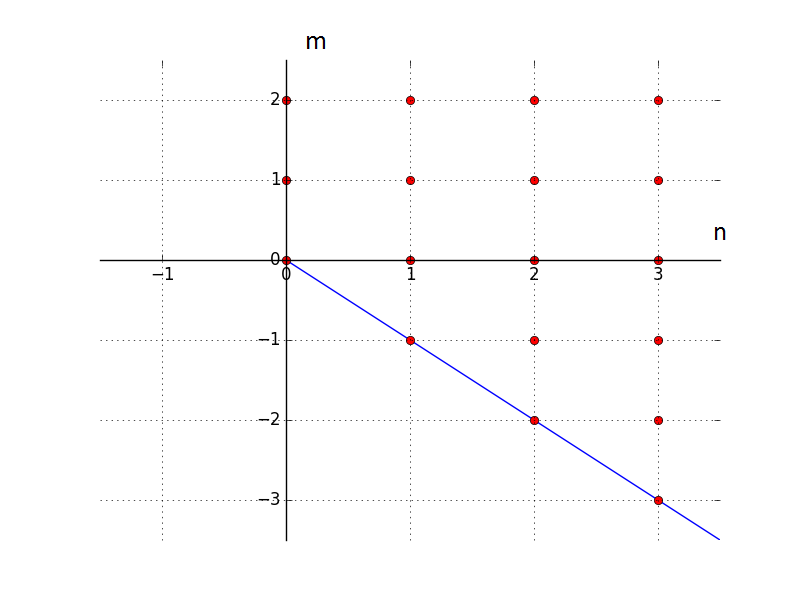
\includegraphics[width=0.5\linewidth]{img/figure_5}
  \captionof{figure}{\emph{Estados de Landau en el gauge simétrico en función de los enteros n y m, tales que n $\geq$ -m.}}
  \label{fig:gauge simetrico}
\end{figure}









\newpage
\leavevmode\thispagestyle{empty}\newpage


%%%%%%%%%%%%%%%%%%%%%%%%%%%%%%%%%%%%%%%%%%%%%
\section{El problema cuántico de Dirac-Landau}
%%%%%%%%%%%%%%%%%%%%%%%%%%%%%%%%%%%%%%%%%%%%% 
$$\\$$








Para plantear el estudio de la ecuación relativista como es la ecuación de Dirac es necesario empezar introduciendo la notación relativista que vamos a utilizar.




$$\\$$%%%%%%%%%%%%%%%%%%%%%%%%%%%%%%%%%%%%%%%%%%%%%%%%%
\textbf{Notación Relativista} 
$$\\$$%%%%%%%%%%%%%%%%%%%%%%%%%%%%%%%%%%%%%%%%%%%%%%%%%





Los postulados de la relatividad nos dicen que la velocidad de la luz en el vacío es la misma en todos los sistemas de referencia inerciales, así como las leyes de la Física (la teoría debe presentar covariancia bajo transformaciones entre estos sistemas), de modo que el espacio en el que suceden los fenómenos físicos es un espacio de dimensión cuatro con una métrica caracterizada por el intervalo espacio-temporal entre dos sucesos: $$\\$$
\begin{equation} \label{eq:3}
s^2=c^2t^2-\vec{x}^{ 2}
\end{equation} \\ \\
De esta forma se define el cuadrivector posición como $$\\$$
\begin{equation}\label{eq:4}
x^\mu=(x^0,x^i) \equiv (ct,\vec{x})
\end{equation} \\ \\
con $\mu$=0,1,2,3 e i=1,2,3 (en general, usaremos indices griegos para referirnos a cuatrivectores y latinos para vectores) tal que $$\\$$
\begin{equation*} %\label{eq:5}
s^2=x^0x^0 - x^i x^i = g_{\mu \nu} x^\mu x^\nu
\end{equation*} $$\\$$
donde usamos el convenio de Einstein de suma de índices repetidos y la métrica o tensor métrico es: $$\\$$
\begin{equation} \label{eq:6}
g_{\mu \nu} = g_{\nu \mu} = diag(1,-1,-1,-1) \qquad .
\end{equation} $$\\$$
El espacio donde suceden los fenómenos físicos es el espacio de Minkowski, $\mathbf{R}^{1,3}$, con una métrica hiperbólica, $g_{\mu \nu}$, y distinta a la usada en el espacio euclídeo, $\delta_{ij}$, propia de la Física no-relativista $$\\$$
\begin{equation*} %\label{eq:7}
\delta_{ij} = diag(1,1,1) \qquad .
\end{equation*} $$\\$$
Los cuadrivectores, $x^\mu$, se transforman contravariantemente con respecto al cambio de coordenadas, se puede definir un cuadrivector covariante como $$\\$$
\begin{equation*}
x_\nu = g_{\nu \mu}x^\mu \qquad . 
\end{equation*} $$\\$$
Las transformaciones de Lorentz son transformaciones lineales en el espacio de Minkowski que mantienen invariante $s^2$, el intervalo entre dos sucesos, es decir $$\\$$
\begin{equation} \label{eq:8}
x^{\mu} \qquad \rightarrow \qquad {x^{'}}^{\mu}={\Lambda^\mu}_\nu x^\nu \qquad,
\end{equation} $$\\$$
con lo cual, se debe cumplir que $$\\$$
\begin{equation*} % \label{eq:9}
g_{\sigma \rho}={\Lambda^\mu}_\sigma {\Lambda^\nu}_\rho g_{\mu \nu} \qquad ,
\end{equation*} $$\\$$
de modo que el conjunto de transformaciones lineales que satisfacen la relación anterior constituyen las transformaciones de  Lorentz: Rotaciones espaciales, Boosts, inversión temporal, paridad e inversión total. En (3+1)-dimensiones los generadores de estas transformaciones satisfacen un álgebra de Lie, y pueden ser identificados con el grupo SO(3+1). Además de la expresión anterior se puede demostrar que las transformaciones homogéneas de Lorentz infinitesimales se puede expresar en función de tensores antisimétricos, y por lo tanto, estas transformaciones están caracterizadas por seis parámetros independientes.   $$\\$$
Otras transformaciones que también dejan invariante el intervalo espacio-temporal, son las traslaciones: $$\\$$
\begin{equation*}  %\label{eq:10}
x^{\mu} \qquad \rightarrow \qquad {x^{'}}^{\mu}=x^\mu + a^\mu \qquad,
\end{equation*} $$\\$$
donde $a^\mu$ es un cuadrivector arbitrario y constante, con lo cual, estas, vienen caracterizadas por 4 parámetros. El grupo de invariancia de la teoría en (3+1)-dimensiones es el grupo de Poincaré, que depende de 10 parámetros: $$\\$$
\begin{equation*} %\label{eq:11}
x^{\mu} \qquad \rightarrow \qquad {x^{'}}^{\mu}={\Lambda^\mu}_\nu x^\nu + a^\mu \qquad .
\end{equation*} $$\\$$
Con todo esto, los operadores diferenciales en (3+1)-dimensiones se escriben como $$\\$$
\begin{equation} \label{eq:12}
\partial_\mu = \frac{\partial}{\partial x^\mu}=(\frac{1}{c}\partial_t,\vec{\nabla} ) \qquad , \qquad \Box = \partial_\mu·\partial^\mu = \frac{1}{c^2}\frac{\partial^2}{\partial t^2} - \nabla^2 \qquad .
\end{equation} $$\\$$
Los operadores cuánticos de momento y energía ahora vienen son descritos por medio del cuatrivector momento $$\\$$
\begin{equation}
\hat{p}_\mu = \left(\frac{\hat{E}}{c}, \hat{p}_1, \hat{p}_2, \hat{p}_3 \right) \equiv i \hbar \partial_\mu \qquad .
\end{equation} $$\\$$







$$\\$$%%%%%%%%%%%%%%%%%%%%%%%%%%%%%%%%%%%%%%%%%%%%%
\subsection{La ecuación de Dirac en el espacio}
$$\\$$%%%%%%%%%%%%%%%%%%%%%%%%%%%%%%%%%%%%%%%%%%%%%









Para obtener las soluciones que describen el comportamiento de fermiones teniendo en cuenta efectos relativistas es necesario recurrir a la ecuación de Dirac. Esta ecuación se deriva de la expresión relativista de la energía sustituyendo las cantidades $E$ y $p^i$ por los operadores canónicos $\hat{E}$ y $\hat{p}^i$, buscando que la densidad de probabilidad de la solución sea positiva [5]$$\\$$
\begin{equation} \label{ecuacion de dirac}
i \frac{\hbar}{c}\frac{\partial}{\partial t} \psi (\vec{x},t) = i \hbar \alpha^i \frac{\partial}{\partial x^i} \psi(\vec{x},t) + \beta mc \psi(\vec{x},t) \qquad ,
\end{equation} $$\\$$
donde los coeficientes $\alpha^i$ y $\beta$ son matrices cuadradas de dimensión 4 denominadas matrices de Dirac, que cumplen $$\\$$
\begin{equation*} 
{\alpha^i}^2 = 1  \hspace{1.5cm}, \hspace{1.5cm} \beta^2 = 1 \qquad \quad {} $$\\$$
\alpha^i \alpha^j + \alpha^j \alpha^i =2 \delta ^{ij}  \hspace{1.5cm}, \hspace{1.5cm} \alpha^i \cdot \beta + \beta \cdot \alpha^i = 0 \qquad .
\end{equation*} $$\\$$
Estas relaciones no definen de manera única las matrices de modo que existen diferentes representaciones posibles para las matrices de Dirac. Las expresiones explícitas de las soluciones depende de estas matrices, por lo que la elección de una determinada representación depende de que expresión sea más conveniente según el problema. No obstante, el teorema fundamental de Pauli permite pasar de una representación a otra. En el caso de una partícula con masa, la elección habitual para $\alpha^i$ y $\beta$ se denomina representación de Dirac, tal que: $$\\$$
\begin{equation} 
\alpha^i = 
\begin{pmatrix}
0 & \sigma_i  \\
 \sigma_i & 0
\end{pmatrix} \hspace{1cm},\hspace{1cm}
\beta=
\begin{pmatrix}
\mathbb{I} & 0 \\
0 & -\mathbb{I}
\end{pmatrix} \qquad ,
\end{equation} $$\\$$
donde $\sigma_i$ (i=1,2,3) son las matrices de Pauli (2x2):  $$\\$$
\begin{equation} 
\sigma_1 = 
\begin{pmatrix}
0 & 1 \\
1 & 0
\end{pmatrix} \qquad, \qquad
\sigma_2=
\begin{pmatrix}
0 & -i \\
i & 0
\end{pmatrix} \qquad , \qquad
\sigma_3=
\begin{pmatrix}
1 & 0 \\
0 & -1
\end{pmatrix} \qquad .
\end{equation} $$\\$$
En esta representación, las cuatro posibles de partícula libre independientes de la ecuación de Dirac de masa m y momento $\vec{p}=(p_1,p_2,p_3)$ son: $$\\$$
\begin{equation} \label{solucion dirac}
\psi_1(\vec{x},t)=N\begin{pmatrix}
1 \\ 0 \\ \frac{c p_3}{E_+ + mc^2} \\ \frac{c(p_1 + ip_2)}{E_+ + mc^2}
\end{pmatrix} e^{\frac{i}{\hbar}(E_+ t - \vec{p}\cdot \vec{x})} \qquad
\psi_2(\vec{x},t)=N\begin{pmatrix}
0 \\ 1  \\ \frac{c(p_1 + ip_2)}{E_+ + mc^2}\\ \frac{c p_3}{E_+ + mc^2}
\end{pmatrix} e^{\frac{i}{\hbar}(E_+ t - \vec{p} \cdot \vec{x})} \quad $$\\$$
\psi_3(\vec{x},t)=N\begin{pmatrix}
\frac{c p_3}{E_- - mc^2} \\ \frac{c(p_1 +ip_2)}{E_- - mc^2}  \\ 1\\ 0
\end{pmatrix} e^{\frac{i}{\hbar}(E_- t - \vec{p} \cdot \vec{x})} \qquad
\psi_4(\vec{x},t)=N\begin{pmatrix}
\frac{-c(p_1- ip_2)}{E_- - mc^2}\\ \frac{-c p_3}{E_- - mc^2} \\ 0 \\ 1  
\end{pmatrix} e^{\frac{i}{\hbar}( E_- t - \vec{p} \cdot \vec{x})} \quad .
\end{equation} $$\\$$
Estas soluciones son objetos matemáticos que se denominan espinores, de cuatro componentes, y que pertenecen al grupo $\textbf{\textit{S}\textit{L}}(2,\mathbb{C})$. Las dos primeras componentes se denominan componentes mayores y las dos últimas menores, esto se deduce del límite no-relativista que veremos más adelantes. Los términos $E_+$ y $E_-$ hacen referencia a los dos posibles soluciones de energía en la expresión relativista: $$\\$$
\begin{equation}
E^2 = m^2c^4 + \vec{p}^2 c^2 \qquad {} $$\\$$
E_+ = +\sqrt{m^2c^4 + \vec{p}^2c^2} \hspace{1.5cm},\hspace{1.5cm} E_- = -\sqrt{m^2c^4 + \vec{p}^2c^2} \qquad,
\end{equation} $$\\$$
de modo que los espinores $\psi_1(\vec{x},t)$ y $\psi_2(\vec{x},t)$ hacen referencia a una partícula con energía $E = E_+$, mientras que $\psi_3(\vec{x},t)$ y $\psi_4(\vec{x},t)$ con $E = E_-$. El coeficiente N es una constante de normalización. Existen dos posibles normalizaciones habituales  [2]$$\\$$
\begin{equation} \label{normalizacion dirac}
· \quad \psi^\dagger \psi =u(\vec{p})_\mu^\dagger u(\vec{p})_\nu=\delta_{\mu\nu} \hspace{1cm} \rightarrow \hspace{1cm} N=\sqrt{(|E|  + mc^2)/2|E|} $$\\$$
· \quad \psi^\dagger \psi = u(\vec{p})_\mu^\dagger u(\vec{p})_\nu= \frac{|E|}{mc^2}\delta_{\mu\nu} \hspace{1cm} \rightarrow \hspace{1cm} N=\sqrt{(|E| + mc^2)/ 2mc^2} \quad.
\end{equation} $$\\$$
Podemos definir el operador de espín $$\\$$
\begin{equation} 
\hat{S_3} \equiv \frac{\hbar}{2}\Sigma_3 = \frac{\hbar}{2} \begin{pmatrix}
\sigma_3 & 0 \\ 0 & \sigma_3
\end{pmatrix} \qquad ,
\end{equation} $$\\$$
siendo $\Sigma_3$ la tercera componente de: $$\\$$
\begin{equation} \label{matriz sigma}
\Sigma_i =  \begin{pmatrix} \sigma_i & 0 \\ 0 & \sigma_i \end{pmatrix} \qquad , \qquad i =1,2,3 \qquad ,
\end{equation} $$\\$$
donde $\Sigma_i$ es una generalización de las matrices de Pauli a un espacio de matrices (4x4). En el caso de que la partícula este en reposo, $\vec{p} = 0$, las funciones de onda (78) son también autoestados del operador $\Sigma_3$. Para el caso en el que la partícula no esté en reposo, el espín no estará bien definido en general, a menos que el movimiento de la partícula sea únicamente en la dirección de la tercera componente $\vec{p} = p\vec{e}_3$. Esto nos dice que aunque las soluciones de partícula libre en movimiento no tienen espín bien definido, podemos construir un operador que nos de la proyección de espín en la dirección del momento. Este operador se denomina helicidad y viene dado por %chapuza \ref{solucion dirac} $$\\$$
\begin{equation} 
\Lambda = \frac{\vec{\sigma} \cdot \vec{p}}{|\vec{p}|} \qquad. 
\end{equation} $$\\$$
Es interesante que en el caso de partículas sin masa el valor de la helicidad coincide con la quiralidad. Para el problema de partícula libre se puede definir una base del espacio tal que $$\\$$
\begin{equation*}
\hat{\Lambda} \psi = \pm  \psi \qquad .
\end{equation*} $$\\$$
Para cálculos posteriores definimos el hermítico conjugado del espinor, que se corresponde con la solución a la ecuación $$\\$$
\begin{equation} \label{eq:29}
\-i\hbar\frac{\partial}{\partial t} \psi ^\dagger = -i \hbar \frac{\partial}{\partial x^i} \psi^\dagger \alpha^i + m \psi^\dagger \beta \; ,
\end{equation} $$\\$$
donde $$\\$$
\begin{equation} \label{eq:30}
\psi ^\dagger (\vec{x},t) = \left(\psi_1^*(\vec{x},t), \psi_2^*(\vec{x},t),\psi_3^*(\vec{x},t),\psi_4^*(\vec{x},t) \right) \;.
\end{equation} $$\\$$ 









$$\\$$%%%%%%%%%%%%%%%%%%%%%%%%%%%%%%%%%%%%%%
\subsubsection{Formulación covariante} 
$$\\$$%%%%%%%%%%%%%%%%%%%%%%%%%%%%%%%%%%%%%%%%








Una ecuación relativista debe ser invariante bajo transformaciones Lorentz. Para comprobarlo, vamos a escribir la ecuación de Dirac en su forma covariante. Multiplicando la ecuación ($\ref{ecuacion de dirac}$) por $\beta$ por la izquierda podemos escribirla de la forma $$\\$$
\begin{equation*} %\label{eq:31}
i\hbar \beta \frac{\partial}{\partial t} \psi = \left[- i \hbar (\beta \alpha^i)\frac{\partial}{\partial x^i} + mc \; \right] \psi \qquad ,
\end{equation*} $$\\$$
de tal manera que en forma covariante $$\\$$
\begin{equation} \label{eq:32}
\left( i \hbar \gamma^\mu \frac{\partial}{\partial x^\mu} - mc \; \right)\psi = (\gamma^\mu p_\mu - mc)\psi=0 \qquad ,
\end{equation} $$\\$$
Se definen las matrices de Dirac, $\gamma^\mu$, como $$\\$$
\begin{equation} \label{eq:33}
\gamma^0= \beta \hspace{1cm} , \hspace{1cm}  \gamma^i=\beta \alpha^i \hspace{1cm} , \hspace{1cm} i=1,2,3\qquad .
\end{equation} $$\\$$ 
A partir de las propiedades que satisfacen las matrices $\alpha^i$ y $\beta$, se deduce que las matrices $\gamma^\mu$ deben cumplir la siguiente relación de anticonmutación $$\\$$
\begin{equation} \label{eq:34}
\gamma^\mu \gamma^\nu + \gamma^\nu \gamma^\mu =2g^{\mu \nu}  \qquad .
\end{equation} $$\\$$
Se define el espinor adjunto $\bar{\psi} = \psi^\dagger \gamma_0$ tal que $$\\$$
\begin{equation} \label{eq:35}
 i \frac{\partial}{\partial x^\mu}\bar{\psi} \gamma^\mu + mc \bar{\psi}=0 \qquad .
\end{equation} $$\\$$







$$\\$$%%%%%%%%%%%%%%%%%%%%%%%%%%%%%%%%%%%%%%%%%%%%%%%%%%%%%%%%%%%%%%%%%
\subsubsection{Acoplamiento con un campo electromagnético} %BETHE 
$$\\$$%%%%%%%%%%%%%%%%%%%%%%%%%%%%%%%%%%%%%%%%%%%%%%%%%%%%%%%%%%%%%%%%%






El acoplamiento entre las partículas descritas por la ecuación de Dirac y el campo electromagnético se hace introduciendo en la ecuación el cuadri-potencial por medio de la sustitución $$\\$$
\begin{equation} \label{acoplamiento minimo}
p_\mu \hspace{2cm} \rightarrow \hspace{2cm} p^{'}_\mu=p_\mu + \frac{e}{c} A_\mu \qquad ,
\end{equation} $$\\$$
donde $p_\mu$ es el cuadrimomento y $A_\mu=(\phi, -\vec{A})$ es el cuadri-potencial vector asociado al campo electromagnético. La introducción del campo de esta forma se denomina \textit{acoplamiento-mínimo}, y asegura la invariancia gauge del sistema. De esta forma la ecuación de Dirac en presencia de un campo electromagnético es: $$\\$$
\begin{equation} \label{eq:61}
\left[\gamma^\mu \left(p_\mu + \frac{e}{c}A_\mu \right)\right]\psi(\vec{x},t)=mc\psi(\vec{x},t) \qquad .
\end{equation} $$\\$$
Esta ecuación contiene toda la información de la interacción de la partícula con un campo electromagnético, pero no de forma explícita, para que así sea multiplicamos la ecuación por sí misma aceptando términos cruzados, de modo que obtenemos una ecuación de segundo orden en derivadas espacio-temporales: $$\\$$
\begin{equation*} %\label{eq:62}
\gamma^\nu \gamma^\mu \left(p_\nu + \frac{e}{c}A_\nu \right)\left(p_\mu + \frac{e}{c}A_\mu \right)\psi(\vec{x},t)=m^2c^2 \psi(\vec{x},t) \qquad .
\end{equation*} $$\\$$
Que también se puede escribir como: [3]$$\\$$ %referecia
\begin{equation}\label{eq:63}  %esta sí
(g^{\mu \nu}-i\sigma_{\mu \nu})\left(p_\mu + \frac{e}{c}A_\mu \right) \left(p_\nu + \frac{e}{c}A_\nu \right)\psi(\vec{x},t)=m^2c^2\psi(\vec{x},t) \qquad ,
\end{equation} $$\\$$
donde hemos definido  $$\\$$
\begin{equation*}% \label{eq:64}
\sigma^{\mu\nu}= \frac{i}{2}[\gamma^\mu , \gamma^\nu] \qquad ,
\end{equation*} $$\\$$
tal que $$\\$$
\begin{equation} \label{eq:65} %esta sí
\Sigma_k=\epsilon_{ijk} \sigma^{ij}   \qquad ,
\end{equation} $$\\$$
donde $\Sigma_k$ son  la generalización de las matrices de Pauli de dimensión 4, definidas en (\ref{matriz sigma}). De modo que desarrollando el miembro de la izquierda de (\ref{eq:63}) utilizando la expresión $$\\$$
\begin{equation*}
\sigma^{\mu \nu}=\frac{1}{2}(\sigma^{\mu \nu} - \sigma^{\nu \mu}) \qquad ,
\end{equation*} $$\\$$
obtenemos $$\\$$
\begin{equation*} %\label{eq:66}
\left(p_\mu + \frac{e}{c}A_\mu \right)\left(p^\mu + \frac{e}{c}A^\mu \right)-\frac{i}{2} \left(\sigma^{\mu \nu}- \sigma^{\nu \mu} \right)\left(p_\mu + \frac{e}{c}A_\mu \right)\left(p_\nu + \frac{e}{c}A_\nu \right) = $$\\$$ = \left(p_\mu + \frac{e}{c}A_\mu \right)\left(p^\mu + \frac{e}{c}A^\mu \right)-\frac{i}{2}\sigma^{\mu \nu}\left[\left(p_\mu + \frac{e}{c}A_\mu \right),\left(p_\nu + \frac{e}{c}A_\nu \right) \right] \qquad .
\end{equation*} $$\\$$
Teniendo en cuenta que $[p_\mu,p_\nu]=[A_\mu, A_\nu]=0$, el conmutador de la expresión anterior se puede escribir como  $$\\$$
\begin{equation} \label{eq:67} %%esta sí
\left[(p_\mu + \frac{e}{c}A_\mu),(p_\nu + \frac{e}{c}A_\nu) \right] = i \frac{e \hbar}{c} ( \partial_\mu A_\nu - \partial_\nu A_\mu)=i \frac{e \hbar}{c} F_{\mu \nu} \qquad ,
\end{equation} $$\\$$
donde $F_{\mu \nu}$ es el tensor electromagnético cuyos elementos son las componentes de los campos electromagnéticos definido como $$\\$$
\begin{equation} \label{eq:68}
F_{\mu \nu} = \partial_\mu A_\nu - \partial_\nu A_\mu \qquad .
\end{equation} $$\\$$
Por ser antisimétrico, lo podemos definir completamente con las componentes: $$\\$$
\begin{equation*} 
F_{0i}=-E_i  \hspace{1cm}, \hspace{1cm} F_{ij}=-\epsilon_{ijk}B_k  \hspace{2.5cm} i,j,k=1,2,3
\end{equation*} $$\\$$
siendo $E_i$ y $B_k$ las componentes del campo eléctrico y magnético respecticamente. Sustituyendo el resultado obtenido en (\ref{eq:67}) en (\ref{eq:63}) $$\\$$
\begin{equation} \label{eq:69} %esta sí
\left[ (p_\mu + \frac{e}{c}A_\mu)(p^\mu + \frac{e}{c}A^\mu) + i \frac{e \hbar}{c}\sigma^{\mu \nu}F_{\mu \nu} \right] \psi(\vec{x},t)=m^2c^2 \psi(\vec{x},t) \qquad .
\end{equation} $$\\$$
usando una de las propiedades de $\sigma^{\mu \nu}$ de (\ref{eq:65}) podemos ver que $$\\$$
\begin{equation*}% \label{eq:70}
\sigma^{0 i} F_{0 i}= \alpha^i E_i \hspace{1.5cm}, \hspace{1.5cm} \sigma^{i j} F_{i j}=\epsilon_{ijk} \Sigma^k B_k \qquad .
\end{equation*} $$\\$$
Los demás términos del producto son nulos por ser $F_{\mu \nu}$ antisimétrico. Finalmente la ecuación (\ref{eq:69}) desarrollada queda $$\\$$
\begin{equation} \label{eq:71} %esta sí
\left[ \left(i \hbar \frac{\partial}{\partial t} + e \phi\right)^2 - \left( \frac{e \hbar}{c} \vec{\nabla} + \frac{e}{c} \vec{A}\right)^2 -   e \hbar c(\vec{\Sigma}\cdot \vec{B} - i \vec{\alpha} \cdot \vec{E})\right]\psi(\vec{x},t)=m^2c^4 \psi(\vec{x},t) \qquad ,
\end{equation} $$\\$$
%la variable $\textit{k}$ es una constante añadida de forma externa para ajustar el factor giromagnético de la interacción espín órbita (en el caso de los electrones no es necesario añadirlo), lo cual está permitido al no afectar a la invariancia gauge.$$\\$$
El hecho de que hayamos multiplicado la ecuación por si misma para el estudio del acoplamiento con un campo externo es debido a que no basta con introducir en la ecuación de Dirac los potenciales electromagnéticos en acoplamiento mínimo  para obtener una ecuación que describa el comportamiento de partículas de espín 1/2, si no que además es necesario obtener una ecuación de segundo orden en derivadas espacio-temporales para que aparezcan explicitamente todos los términos.  $$\\$$
Analizaremos el límite no-relativista de este sistema. Para ello es necesario utilizar una representación concreta y tomaremos la de Dirac. Escribimos la ecuación de Dirac, ahora también, de la forma (\ref{eq:71}), con la separación explícita entre las coordenadas espaciales y temporales, como una ecuación matricial para las componentes mayores y menores del espinor $\psi(\vec{x},t)$: $$\\$$
\begin{equation} \label{componentes mayores y menores 3D}
\psi(\vec{x},t) = 
\begin{pmatrix} \psi_a(\vec{x},t) \\ \psi_b(\vec{x},t) \end{pmatrix}  \qquad .
\end{equation} $$\\$$
Si además asumimos los potenciales $\phi$ y $\vec{A}$ como estáticos tenemos $$\\$$
\begin{equation} \label{eq:72}
\begin{pmatrix}
E + e\phi - mc^2 & -\sigma^i(cp_i + e A_i) \\ -\sigma^i(cp_i + eA_i) & E + e\phi + mc^2
\end{pmatrix} \begin{pmatrix}
\psi_a(\vec{x}) \\ \psi_b (\vec{x})
\end{pmatrix} = 0 \qquad ,
\end{equation} $$\\$$
que se puede escribir como un sistema de dos ecuaciones acopladas $$\\$$
\begin{equation*}% \label{eq:73}
\sigma^i (cp_i + eA_i)\psi_b(\vec{x}) - mc^2 \psi_a(\vec{x}) = (E + e\phi) \psi_a(\vec{x}) \qquad  $$\\$$
\sigma^i (cp_i + eA_i)\psi_a(\vec{x}) + mc^2 \psi_b(\vec{x}) = (E + e\phi)\psi_b(\vec{x}) \qquad .
\end{equation*} $$\\$$
Hacemos el cambio $E=E' + mc^2$ y despejamos $\psi_b(\vec{x})$ de la segunda ecuación y sustituimos en la primera, de modo que se obtiene una ecuación de segundo orden desacoplada para las componentes mayores $$\\$$
\begin{equation*} %\label{eq:74}
\frac{1}{2mc^2}\sigma^i(cp_i + eA_i)\left(1 + \frac{E+e\phi}{2mc^2}\right)^{-1} \sigma^i(cp_i + eA_i) \psi_a(\vec{x})=(E' - e\phi)\psi_a(\vec{x}) \qquad.
\end{equation*} $$\\$$
Los cálculos hechos hasta ahora son exactos. Reescribimos la ecuación anterior con la aproximación del régimen no-relativista $$\\$$
\begin{equation} \label{eq:75}
E'<<mc^2 \hspace{1cm}, \hspace{1cm} e\phi <<mc^2  \quad \rightarrow \quad \frac{E+e \phi}{2mc^2}\simeq 0 \qquad ,
\end{equation} $$\\$$
y además despreciamos términos proporcionales a $(v/c)$, por lo que las componentes menores, $\psi_b\propto (v/c)\psi_a$, se desprecian en esta aproximación. Con esto la ecuación en aproximación no-relativista es $$\\$$
\begin{equation} \label{eq:76}
\left[\frac{1}{2m}\left( \vec{p} + \frac{e}{c}\vec{A}\right)^2 - e \phi + \frac{e \hbar}{2mc} \vec{\sigma}\cdot\vec{B} \right] \psi_a(\vec{x})=E' \; \psi_a(\vec{x}) \qquad .
\end{equation} $$\\$$
Esta es la ecuación de Pauli para espinores de dos componentes, que tiene en cuenta el espín en la mecánica cuántica no-relativista. El término con el campo magnético constituye la energía de interacción dipolar magnética con un factor giromagnético de valor 2 de manera natural, el cual es propio de los electrones.  $$\\$$
%Al igual que antes, podemos introducir una factor $k$ para ajustar el valor del factor giromagnético al valor experimental para otras partículas. \\ \\
Otra aproximación interesante para un campo electroestático constante ($\vec{A}=0$) consiste en realizar lo mismo, pero manteniendo ahora los términos proporcionales a $(v^2/c^2)$, por lo que  $$\\$$
\begin{equation*} %\label{eq:77}
\left(1 + \frac{E+e\phi}{2mc^2}\right)^{-1} \simeq \left(1 - \frac{E+e\phi}{2mc^2}\right) \qquad .
\end{equation*} $$\\$$
Si además el potencial tiene simetría esférica, $\phi(\vec{x})=\phi(r)$, y añadimos la condición de que $E'+e\phi \simeq p^2/2m$ $$\\$$
\begin{equation} \label{eq:78}
\left[\frac{p^2}{2m} - e\phi - \frac{p^4}{8m^3c^2} + \frac{e\hbar^2}{4m^2c^2}\frac{d\phi}{dr}\frac{\partial}{\partial r} - \frac{e}{2m^2c^2}\frac{1}{r} \frac{d\phi}{dr} \vec{S} \cdot \vec{L}\right] \psi_a(r)=E' \; \psi_a(r) \qquad .
\end{equation} $$\\$$
Los dos primeros términos están presentes en la ecuación de Schroedinger. El tercer término es una corrección relativista a la energía cinética y el cuarto es un término sin análogo clásico. El último término es la contribución de la interacción espín-órbita [3]. $$\\$$









$$\\$$%%%%%%%%%%%%%%%%%%%%%%%%%%%%%%%%%%%%%%%%%%%%%
\subsection{La ecuación de Dirac-Landau en el espacio} 
$$\\$$%%%%%%%%%%%%%%%%%%%%%%%%%%%%%%%%%%%%%%%%%%%%%









En este apartado vamos a resolver la ecuación de Dirac en presencia de un campo magnético constante $\vec{B} = B \vec{e}_3$. Para ello introducimos el potencial vector del campo, como vimos en la expresión (\ref{acoplamiento minimo}) $$\\$$
\begin{equation*}
\vec{p} \hspace{2cm} \longrightarrow \hspace{2cm} \vec{p} \: ' = \vec{p} + \frac{e}{c}\vec{A}  \qquad ,
\end{equation*} $$\\$$
donde $$\\$$
\begin{equation*}
\vec{A} = (-\frac{B}{2} x^2, \frac{B}{2} x^1,0) \qquad .
\end{equation*} $$\\$$
Hemos elegido el gauge simétrico para el potencial vector que describe el campo magnético, $A_i$, aunque también sería posible haber elegido el gauge de Landau. De esta forma la ecuación matricial de autovalores para los estados es: $$\\$$
\begin{equation*}
\hat{H} \psi(\vec{x}) = E \psi (\vec{x}) \hspace{1.5cm}, \hspace{1.5cm}
\begin{pmatrix}
mc^2 & \sigma_i (c\hat{p}_i + e{A}_i) \\
 \sigma_i(c\hat{p}_i + e{A}_i) & -mc^2
\end{pmatrix} \psi(\vec{x}) = E \psi(\vec{x}) \qquad .
\end{equation*} $$\\$$
Esta ecuación matricial nos da un sistema de ecuaciones acopladas para las componentes mayores y menores, ($\psi_a$ y $\psi_b$), del espinor. El potencial vector $\vec{A}$ depende de las coordenadas $x^1$ y $x^2$, por lo que ahora, el espinor solo van a poder ser autoestados de una componente del momento $p_3$. $$\\$$
\begin{equation} \label{dirac-landau acoplado}
\begin{cases}
mc^2 \psi_a  + \sigma^i(c\hat{p}_i + e {A}_i)\psi_b = E \psi_a \qquad \quad {}$$\\$$
\sigma^i(c\hat{p}_i + e {A}_i)\psi_a - mc^2 \psi_b = E \psi_b \end{cases} \qquad .
\end{equation} $$\\$$
Despejamos $\psi_b$ de la segunda ecuación y sustituimos en la primera desacoplando así el sistema en una ecuación de segundo orden para $\psi_a$. $$\\$$
\begin{equation*}
\psi_a = \frac{1}{E^2-m^2c^4}\sigma^i(c\hat{p}_i + e{A}_i)\sigma^i(c\hat{p}_i + e{A}_i)\psi_a \qquad {}$$\\$$
[(c\hat{p}_i + e{A}_i)^2  + eB \hbar c^2 \sigma^3 ] \psi_a = (E^2 - m^2c^4) \psi_a  \qquad {} $$\\$$
[c^2\hat{p}_i\hat{p}_i + e^2{A}^2 + ec^2 L_3 B + e B \hbar c^2 \sigma^3]\psi_a = (E^2 - m^2c^4) \psi_a \qquad {} $$\\$$
[ c^2 \hat{p}_i\hat{p}_i + e^2{A}^2 + e B c^2 J_3 ]\psi_a = (E^2 - m^2c^4) \psi_a $$\\$$
\left[c^2{p_3}^2 +c^2\left(\frac{\partial^2}{\partial {x_1}^2} + \frac{\partial^2}{\partial {x_2}^2}\right)+ e^2{A}^2 + e B c^2 J_3  \right]\psi_a = (E^2 - m^2c^4) \psi_a\qquad . 
\end{equation*} $$\\$$
En la segundo paso hemos aplicado que, en este guage, la divergencia del potencial vector es nula y la definición del operador $\hat{L}_3 = \hat{x}_2\hat{p}_1 -\hat{x}_1\hat{p}_2$. En el primer paso hemos utilizado la siguiente propiedad de las matrices $\sigma^i$ operando sobre dos vectores $P_i$ y $Q_i$ $$\\$$
\begin{equation}
(\sigma^i P_i)(\sigma^i Q_i) = P^i Q_i + i \sigma^i \epsilon_{jki}P_j Q_k \qquad . 
\end{equation} $$\\$$
De esta forma hemos obtenido explicitamente la tercera componente del operador momento angular total $J_3$ dado por: $$\\$$
\begin{equation*}
\hat{J}_3 = \hat{L}_3 + \hat{S}_3 = \hat{x}_2\hat{p}_1 -\hat{x}_1\hat{p}_2 + \frac{\hbar}{2} \sigma^3 \qquad .
\end{equation*}$$\\$$
Teniendo en cuenta la forma del término de la izquierda de la expresión para $\psi_a$, podemos escribirlo como $$\\$$
\begin{equation} \label{diraclandau descomposicion}
\left[c^2{p_3}^2 +c^2\left(\frac{\partial^2}{\partial {x_1}^2} + \frac{\partial^2}{\partial {x_2}^2}\right)+ e^2{A}^2 + e B c^2 J_3  \right]\psi_a = (E^2 - m^2c^4) \psi_a\qquad {} $$\\$$ 
[\hat{H}_{libre}(x^3) + 2mc^2 \hat{H}_{sym}(x^1,x^2) + \hat{H}_{spin}] \psi_a = (E^2 - m^2c^4)\psi_a\qquad .
\end{equation} $$\\$$
El primer término hace referencia al movimiento libre en la dirección perpendicular al plano, es decir la dirección del campo magnético, el segundo es el comportamiento de oscilador de una partícula, en el plano perpendicular al campo magnético, y el tercero, es la interacción del espín de la partícula con el campo magnético. Como hemos dicho, el Hamiltoniano depende del espín, por lo que la estructura de niveles energéticos será diferente según los autovalores del espín. De esta forma los autovalores de la energía vienen dados por $$\\$$
\begin{equation}
E^2 - m^2c^4 = c^2 p_3^2 + 2mc^2 \hbar w_c \left(n + \frac{1}{2}\right) \pm e\hbar c^2  B \qquad \quad {} $$\\$$
E_{\pm}^{\uparrow} = \pm  \sqrt{m^2c^4 + c^2 p_3^2 + 2mc^2 \hbar w_c \left(n + \frac{1}{2}\right) + e\hbar c^2  B} \qquad {} $$\\$$
E_{\pm}^{\downarrow} = \pm  \sqrt{m^2c^4 + c^2 p_3^2 + 2mc^2 \hbar w_c \left(n + \frac{1}{2}\right) - e\hbar c^2  B} \qquad .
\end{equation} $$\\$$
Ademas, $E_{\pm}^{\uparrow}$ y $E_{\pm}^{\downarrow}$ dependen del número cuántico $n = 0,1,2,..$y de  $p_3 \in (-\infty, \infty)$. Al definir la energía de forma cuadrática, tenemos dos posibles signos para el valores de la energía para cada valor de espín. Los niveles energéticos de los estados con valor de espín positivo vienen dados por $E_{\pm}^{\uparrow}$, mientras que los que tienen espín negativo vienen dados por $E_{\pm}^{\downarrow}$. $$\\$$
Continuando con la expresión (105), podemos obtener la expresión para los espinores propios del Hamiltoniano. Buscamos espinores de la forma  $$\\$$ %chapuza \ref{diraclandau descomposicion} 
\begin{equation}
\psi_a = \begin{pmatrix}
\psi_{a1} \\ \psi_{a2}
\end{pmatrix} 
\psi_{n,m}(x^1,x^2) e^{-\frac{i}{\hbar}p_3x^3} \qquad ,
\end{equation} $$\\$$
donde $\psi_{n,m}$ es un autoestado del Hamiltoniano de Schroedinger acoplado a un campo magnético uniforme en el gauge simétrico, visto en la sección anterior. Sustituyendo esta expresión en la ecuación para $\psi_a$, resulta:  $$\\$$
\begin{equation*}
\begin{pmatrix}
(c\vec{p} + e\vec{A})^2 - e\hbar c^2B & 0 \\ 0 & (c\vec{p} + e\vec{A})^2 + e\hbar c^2B
\end{pmatrix}
\begin{pmatrix}
\psi_{a1} \\ \psi_{a2}
\end{pmatrix} = (E^2 - m^2c^4) 
\begin{pmatrix}
\psi_{a1} \\ \psi_{a2}
\end{pmatrix} \qquad.
\end{equation*} $$\\$$
Las ecuaciones para las componentes espinoriales están desacopladas, por tanto, podemos escoger los espinores de Pauli como solución. $$\\$$
\begin{equation*}
\psi_a = \begin{pmatrix}
1 \\ 0
\end{pmatrix} 
\psi_{n,m}(x^1,x^2) e^{-\frac{i}{\hbar}p_3x^3} \hspace{2cm}, \hspace{2cm}
\psi_a = \begin{pmatrix}
0 \\ 1
\end{pmatrix} 
\psi_{n,m}(x^1,x^2) e^{-\frac{i}{\hbar}p_3x^3} 
\end{equation*} $$\\$$
Una vez obtenidas las componentes mayores, $\psi_a$, vamos a obtener las componentes menores, $\psi_b$, por medio de la segunda ecuación de (\ref{dirac-landau acoplado}) $$\\$$
\begin{equation*}
\sigma^i (cp_i + eA_i)\psi_a = (E + mc^2) \psi_b \qquad {} $$\\$$
\begin{pmatrix}
c p_3  & (c p_2 +eA_2) + i(cp_1 + eA_1) \\ (cp_2 +eA_2) -i (cp_1 + eA_1) & cp_3c
\end{pmatrix} \psi_a = 
(E+mc^2)\psi_b \qquad .
\end{equation*} $$\\$$
Definimos los operadores [31] $$\\$$
\begin{equation} \label{operadoresD}
D = \sqrt{2ec \hbar B}\; \hat{a}^\dagger \hspace{1.5cm}, \hspace{1.5cm} D^\dagger = - \sqrt{2ec\hbar B}\; \hat{a} \qquad ,
\end{equation} $$\\$$
$\hat{a}$ y $\hat{a}^\dagger$ actuan sobre $\psi_{n,m}$ como vimos en la sección anterior (60), de modo que la expresión anterior se puede escribir como $$\\$$ %chapuza \ref{actuacion escalera}
\begin{equation*}
\begin{pmatrix}
cp_3 & D \\ D^\dagger & cp_3
\end{pmatrix}
\psi_a = (E+mc^2)\psi_b \qquad \quad {} $$\\$$
\psi_b = \frac{1}{E+mc^2}
\begin{pmatrix}
cp_3 & D \\ D^\dagger & cp_3
\end{pmatrix}
\begin{pmatrix}
\psi_{a1}  \\
\psi_{a2} 
\end{pmatrix} \psi_{n,m}e^{-\frac{i}{\hbar}p_3x^3} \qquad \quad {} $$\\$$
\psi_b = \frac{1}{E+mc^2}
\begin{pmatrix}
cp_3 \psi_{a1} \psi_{n,m} + \sqrt{2ec\hbar B} \psi_{a2} \sqrt{n+1} \psi_{n+1,m-1} \\
-\sqrt{2ec\hbar B}\psi_{a1} \sqrt{n} \psi_{n-1,m+1} + cp_3 \psi_{a2} \psi_{n,m}
\end{pmatrix}
e^{-\frac{i}{\hbar}p_3x^3} \qquad .
\end{equation*} $$\\$$
Para una elección de las componentes mayores, las componentes menores se escriben como $$\\$$
\begin{equation*}
\psi_a = \begin{pmatrix} 1 \\ 0 \end{pmatrix} \psi_{n,m} e^{-\frac{i}{\hbar}p_3x^3} \hspace{1cm} \rightarrow \hspace{1cm} 
\psi_b = \frac{1}{E + mc^2} \begin{pmatrix}
cp_3 \; \psi_{n,m} \\
-\sqrt{2ec\hbar B n} \; \psi_{n-1,m +1} 
\end{pmatrix} e^{-\frac{i}{\hbar}p_3x^3} \qquad \quad {} $$\\$$
\psi_a = \begin{pmatrix} 0 \\ 1 \end{pmatrix} \psi_{n,m} e^{-\frac{i}{\hbar}p_3x^3} \hspace{1cm} \rightarrow \hspace{1cm} 
\psi_b = \frac{1}{E + mc^2} \begin{pmatrix}
\sqrt{2ec\hbar B(n+1)} \; \psi_{n+1,m-1}  \\
cp_3 \; \psi_{n,m}
\end{pmatrix} e^{- \frac{i}{\hbar}p_3x^3} \qquad .
\end{equation*} $$\\$$
Los estados propios, por tanto, se escriben como: $$\\$$
\begin{equation}
\psi_1(\vec{x},t) = N \begin{pmatrix}
\psi_{n,m} \\ 
0 \\
\frac{cp_3 }{E_{+}^\uparrow + mc^2} \psi_{n,m}\\
\frac{-\sqrt{2eB\hbar c n } }{E_+^\uparrow + mc^2}\psi_{n-1,m +1}
\end{pmatrix} e^{-\frac{i}{\hbar}(p_3x^3 - E_+^\uparrow t)} \qquad , $$\\$$
\psi_2(\vec{x},t) = N \begin{pmatrix}
0 \\ 
\psi_{n,m} \\
\frac{\sqrt{2eB\hbar c (n+1)}  }{E_+^\downarrow + mc^2}\psi_{n+1,m-1} \\
\frac{cp_3 }{E_+^\downarrow + mc^2} \psi_{n,m}
\end{pmatrix} e^{-\frac{i}{\hbar}(p_3x^3 -E_+^\downarrow t)} \qquad ,
\end{equation} $$\\$$
donde $\psi_{n,m} \equiv \psi_{n,m}(x^1,x^2)$. La constante N es una constante de normalización que viene dada por $$\\$$
\begin{equation}
\int \psi^\dagger (\vec{x})\psi (\vec{x}) d^3x = 1 \qquad .
\end{equation} $$\\$$
Estas soluciones se corresponden con aquellas de energía positiva, $E_+^\uparrow$ y $E_+^\downarrow$ respectivamente. Podemos obtener otras dos soluciones para el valor de energía negativa, para ello resolvemos el sistema (103) desacoplando las ecuaciones para $\psi_b$, es decir:  $$\\$$ %chapuza (\ref{dirac-landau acoplado}) $$\\$$
\begin{equation*}
\psi_b = \begin{pmatrix} \psi_{b1} \\ \psi_{b2} \end{pmatrix} \psi_{n,m} e^{-\frac{i}{\hbar} p_3 x^3} \qquad .
\end{equation*} $$\\$$
Despejando $\psi_a$ de la primera ecuación de (\ref{dirac-landau acoplado}), obtenemos el correspondiente valor de $\psi_a$ $$\\$$
\begin{equation*}
\psi_b = \begin{pmatrix} 1 \\ 0 \end{pmatrix} \psi_{n,m} e^{-\frac{i}{\hbar}p_3x^3} \hspace{1cm} \rightarrow \hspace{1cm} 
\psi_a = \frac{1}{E - mc^2} \begin{pmatrix}
cp_3 \; \psi_{n,m} \\
-\sqrt{2ec\hbar B n}\; \psi_{n-1,m +1} 
\end{pmatrix} e^{-\frac{i}{\hbar}p_3x^3} \qquad \quad {} $$\\$$
\psi_b = \begin{pmatrix} 0 \\ 1 \end{pmatrix} \psi_{n,m} e^{-\frac{i}{\hbar}p_3x^3} \hspace{1cm} \rightarrow \hspace{1cm} 
\psi_a = \frac{1}{E - mc^2} \begin{pmatrix}
\sqrt{2ec\hbar B (n+1)}\;  \psi_{n+1,m-1}  \\
cp_3 \; \psi_{n,m}
\end{pmatrix} e^{- \frac{i}{\hbar}p_3x^3} \qquad .
\end{equation*} $$\\$$
Las soluciones completas son $$\\$$
\begin{equation}
\psi_3(\vec{x},t) = N \begin{pmatrix}
-\frac{cp_3 }{E_-^\uparrow + mc^2}\psi_{n,m} \\
\frac{\sqrt{2eB\hbar c n }  }{E_-^\uparrow + mc^2} \psi_{n-1,m +1}\\
\psi_{n,m} \\
0
\end{pmatrix} e^{-\frac{i}{\hbar}(p_3x^3 - E_-^\uparrow - t)} \qquad , $$\\$$
\psi_4(\vec{x},t) = N \begin{pmatrix}
\frac{-\sqrt{2eB\hbar c (n+1) } }{E_-^\downarrow + mc^2} \psi_{n+1,m-1} \\
-\frac{cp_3}{E_-^\downarrow + mc^2} \psi_{n,m} \\
0 \\
\psi_{n,m}
\end{pmatrix} e^{-\frac{i}{\hbar}(p_3x^3 - E_-^\downarrow t)} \qquad .
\end{equation} $$\\$$
En este caso, estas soluciones se corresponden con los niveles energéticos $E_-^\uparrow$ y $E_-^\downarrow$ respectivamente. En el problema de Dirac-Landau seguimos obteniendo, como en el problema de partícula libre relativista, soluciones para ambos signos de la energía, sin embargo, no obtenemos soluciones que sean también autoestados del operador de espín, o bien, del operador helicidad. En el problema no-relativista de Landau, en el gauge simétrico, vimos que los estados propios del Hamiltoniano eran propios también del momento angular en la dirección del campo magnético, $\hat{L}_3$, con autovalor $\hbar m$, y esto caracterizaba la degeneración de cada nivel de Landau. En el problema relativista de Dirac-Landau en el gauge simétrico, los niveles de Dirac-Landau también están degenerados en $m$, pero los espinores ya no son propios de $\hat{L}_3$, sino que se mezclan componentes con diferentes valores de $m$. En la teoría de Dirac lo que se conserva no es el momento angular, sino el momento angular total, $\hat{J}_3$. $$\\$$ 
Para campos magnéticos suficientemente pequeños i.e: $$\\$$
\begin{equation*}
\left|\frac{\sqrt{2ec\hbar B}}{E_{\pm}^{\uparrow \downarrow}+mc^2}\right| << 1 \qquad ,
\end{equation*} $$\\$$
podemos escribir los estados propios como $$\\$$
\begin{equation*}
\psi(\vec{x},t) = N \begin{pmatrix} 1 \\0 \\ \frac{cp_3 }{E_{+}^\uparrow + mc^2}\\0  \end{pmatrix} \psi_{n,m} e^{\frac{i}{\hbar}( E_{+}^\uparrow t - p_3x^3 )} \hspace{1cm} , \hspace{1cm}
\psi(\vec{x},t) = N \begin{pmatrix} 0 \\ 1 \\0 \\ \frac{cp_3 }{E_{+}^\downarrow + mc^2} \end{pmatrix} \psi_{n,m} e^{\frac{i}{\hbar}(E_{+}^\downarrow t - p_3x^3 )} \qquad \quad {} $$\\$$
\psi(\vec{x},t) = N \begin{pmatrix} \frac{-cp_3 }{E_{-}^\uparrow + mc^2} \\0\\1 \\0\end{pmatrix} \psi_{n,m} e^{\frac{i}{\hbar}(E_{-}^\uparrow t - p_3x^3)} \hspace{1cm} , \hspace{1cm}
\psi(\vec{x},t) = N \begin{pmatrix} 0 \\ \frac{-cp_3}{E_{-}^\downarrow + mc^2}  \\0 \\ 1 \end{pmatrix} \psi_{n,m} e^{\frac{i}{\hbar}(E_{-}^\downarrow t - p_3x^3 )} \qquad .
\end{equation*} $$\\$$
Como vemos, para campos suficientemente débiles, comprobamos que los estados son propios de $\hat{J}_3 = \hat{L}_3 + \hat{S}_3$. $$\\$$ $$\\$$


\textbf{Degeneración de los niveles energéticos} $$\\$$ 



Los niveles energéticos en el problema relativista de una partícula en presencia de un campo magnético uniforme también están degenerados, de igual manera que en el problema no-relativista. Esa degeneración depende del gauge elegido, que como hemos visto puede ser el gauge simétrico o el de Landau. $$\\$$
En este caso concreto, es decir, si elegimos el gauge simétrico, la degeneración es debida a que fijado un valor de $n$ los posibles valores de $m$ son $$\\$$
\begin{equation*}
-n \leq m \leq \infty \qquad .
\end{equation*} $$\\$$
Teniendo en cuenta que la expresión de la energía no depende de $m$ tenemos una degeneración infinita discreta, a diferencia de la que obteníamos en el gauge de Landau, que era una degeneración continua e infinita en $p_1$. El número de estados posibles con la misma energía en ambos casos es: $$\\$$
\begin{equation*}
n^\circ \quad de \quad estados = \frac{L_1 L_2}{h c} e B \qquad . 
\end{equation*} $$\\$$
$L_1L_2$ es el área finita en la que imponemos condiciones de contorno periódicas. Este resultado es esencial, como veremos más adelante, para entender el Efecto Hall Cuántico.






\newpage





%%%%%%%%%%%%%%%%%%%%%%%%%%%%%%%%%%%%%%%%%%%%%%%%%%%%
\subsection{La ecuación de Dirac en el plano} 
$$\\$$%%%%%%%%%%%%%%%%%%%%%%%%%%%%%%%%%%%%%%%%%%%%%%%%%%%%%%%%










Para el caso de (2+1)-dimensiones buscamos una ecuación relativista con los mismos requisitos que impusimos en el caso de (3+1)-dimensiones. Por lo tanto, podría parecer que una restricción del resultado anterior a una dimensión menor sería suficiente, pero no es así. Aunque la forma de la ecuación debe ser la misma que (\ref{ecuacion de dirac}), los coeficientes no serán los mismos, ya que la reducción del número de coordenadas implica una reducción del número de relaciones de anticonmutación. De modo que ahora la expresión $$\\$$
\begin{equation} \label{eq:115}
\alpha^j  \alpha ^i + \alpha^i  \alpha^j = 2\delta _{ij} \quad ,
\end{equation} $$\\$$
solo nos da dos relaciones de anticonmutación (i=1,2). En total tendremos tres relaciones de anticonmutación, las cuales se pueden satisfacer con las matrices de Pauli de dimensión 2x2, por lo que para el caso de (2+1)-dimensiones los coeficientes $\alpha^i$ y $\beta$ son matrices cuadradas de dimensión 2, así como las matrices $\gamma^\mu$, $\mu = 0,1,2$. Con esto, la solución de la ecuación de Dirac en (2+1)-dimensioes $\psi(\vec{x},t)$ ahora será un espinor de dos componentes. $$\\$$
Una vez definidos los coeficientes, la restricción al plano, consiste restringir el movimiento a una superficie en la que una de las coordenadas espaciales permanece constante, pasando a ser prescindible. De esta forma introducimos la notación para el problema en (2+1)-dimensiones de la misma manera que en la sección anterior, suprimiendo una de las coordenadas espaciales.  $$\\$$
\begin{equation} \label{eq:116}
g_{\mu \nu}=diag(1,-1,-1) \hspace{2.5cm} x^\mu \equiv (ct,\vec{x}) =(x^0,x^1,x^2) $$\\$$
\partial_\mu = \frac{\partial}{\partial x^\mu}=(\frac{1}{c}\partial_t,\partial_1, \partial_2 ) \hspace{2.5cm} \Box = \partial_\mu·\partial^\mu = +\frac{1}{c^2}\frac{\partial^2}{\partial t^2} - \frac{\partial^2}{\partial x_1^2} - \frac{\partial^2}{\partial x_2^2} \qquad ,
\end{equation} $$\\$$
donde $\mu=0,1,2$ y $\vec{x}=(x_1,x_2)$, de modo que los vectores covariantes pasan a ser trivectores. $$\\$$
Del mismo modo que en el caso de (3+1)-dimensiones definimos el espinor adjunto para (2+1)-dimensiones así como la densidad de corriente como $$\\$$
\begin{equation} \label{eq:117}
\bar{\psi}(\vec{x},t)= \psi^\dagger (\vec{x},t) \beta \hspace{1.5cm},\hspace{1.5cm} \hat{p}_\mu \bar{\psi}\gamma^\mu  + mc \bar{\psi}=0 \qquad {} $$\\$$
j^\mu=e c \bar{\psi}\gamma^\mu \psi = (c\rho , j^1, j^2, j^3) \qquad ,
\end{equation} $$\\$$











$$\\$$%%%%%%%%%%%%%%%%%%%%%%%%%%%%%%%%%%%%%%%%%%%%%%%%%%%%%%%%%%%%%%
\subsubsection{Representaciones irreducibles de las matrices gamma} $$\\$$
$$\\$$%%%%%%%%%%%%%%%%%%%%%%%%%%%%%%%%%%%%%%%%%%%%%%%%%%%%%%%%%%%%%%%%%









A pesar de que el número de matrices 2x2 que cumplen los requisitos es el mismo que el número de matrices que buscamos, existe más de una posible representación para las matrices $\gamma^\mu$. Por analogía, tomaremos como representación de Dirac en (2+1)-dimensiones aquella en la que la matriz $\gamma^0$ es diagonal.
\begin{itemize}


\item Representación A \\ \\
\begin{equation}
\gamma^0=\sigma_3 \hspace{1cm} , \hspace{1cm} \gamma^1=i\sigma_1 \hspace{1cm}, \hspace{1cm} \gamma^2=i\sigma_2 \qquad .
\end{equation}\\ \\
También es interesante considerar otra representación en la que $\gamma^0$ es diagonal:\\ 


\item Representación B \\ \\
\begin{equation}
\gamma^0=\sigma_3 \hspace{1cm}, \hspace{1cm} \gamma^1=i\sigma_1 \hspace{1cm}, \hspace{1cm} \gamma^2=-i\sigma_2 \quad .
\end{equation} \\
\end{itemize}
Las matrices $\alpha^i$ y $\beta$ para cada representación se pueden obtener invirtiendo las expresiones obtenidas en (\ref{eq:33}). $$\\$$
El motivo de introducir otra representación, como veremos más adelante, es que ambas representaciones no son equivalentes, o lo que es lo mismo, las soluciones obtenidas para la ecuación de Dirac en cada representación no son las mismas. $$\\$$
Una ecuación relativista que describa partículas de espín 1/2 tiene cuatro soluciones linealmente independientes, resultado de las posibles combinaciones de las dos posibles soluciones de energía y de espín. En el caso de (3+1)-dimensiones cualquier representación nos da espinores de dimensión cuatro con lo que es posible obtener cuatro soluciones linealmente independientes para cualquier representación. En el caso de (2+1)-dimensiones no es así, y como veremos, la única forma de obtener todas las posibles soluciones es combinando las dos representaciones. $$\\$$
Más adelante veremos que es posible encontrar una transformación unitaria que nos relacione las dos representaciones, con lo cual, podemos pasar de los espinores obtenidos en una representación a otros equivalentes en la otra representación.









$$\\$$%%%%%%%%%%%%%%%%%%%%%%%%%%%%%%%%%%%%%%%%%%%%%%%%%%%%%%%%%%%%%%%%%%%%%%%%%%%%%%%%%%%%%%%%%%%%%%%%
\subsubsection{Soluciones de partícula libre en el plano en ambas representaciones: espín} $$\\$$
$$\\$$%%%%%%%%%%%%%%%%%%%%%%%%%%%%%%%%%%%%%%%%%%%%%%%%%%%%%%%%%%%%%%%%%%%%%%%%%%%%%%%%%%%%%%%%%%%%%%%%%








Como vimos en (3+1)-dimensiones, la ecuación de Dirac admite soluciones de onda plana para la partícula libre, ahora en (2+1)-dimensiones también tenemos soluciones de onda plana, pero con espinores de dos componentes. Podemos obtener un sistema de ecuaciones para las componentes del espinor la solución de onda plana en cada representación de las matrices gamma.


$$\\$$
\textbf{Representación A} \\ 
$$\\$$


Para soluciones estacionarias de la ecuación de Dirac de partícula libre, el Hamiltoniano nos da un sistema de ecuaciones en forma matricial como  $$\\$$
\begin{equation*} \label{eq:120}
\begin{pmatrix}
mc^2 & c(ip_1+p_2) \\ c(ip_1-p_2) & -mc^2
\end{pmatrix} 
\begin{pmatrix}
u_{A1}(\vec{p}) \\ u_{A2}(\vec{p})
\end{pmatrix}= E
\begin{pmatrix}
u_{A1}(\vec{p}) \\ u_{A2}(\vec{p})
\end{pmatrix}
 \quad ,
\end{equation*} $$\\$$
donde $u_{A1}(\vec{p})$ y $u_{A2}(\vec{p})$ son las componentes del espinor en la representación A, $u_A(\vec{p})$. El sistema tiene dos soluciones distintas de la trivial linealmente independientes para cada signo de la energía. Si para energía positiva, $E=E_+$, tomamos $u_{A1}=1$ y resolvemos en $u_{A2}$ y para energía negativa, $E=E_-$, tomamos $u_{A2}=1$ y resolvemos en $u_{A1}$, obtenemos: $$\\$$
\begin{equation*} \label{eq:121}
u_{A}(\vec{p})= N\begin{pmatrix}
1 \\ \frac{c(ip_1+ p_2)}{E_+ +mc^2}
\end{pmatrix} \hspace{2.5cm} , \hspace{2.5cm}
u_{A} (\vec{p})= N\begin{pmatrix}
\frac{c(p_2 + i p_1)}{E_- -mc^2} \\ 1
\end{pmatrix} \qquad ,
\end{equation*} $$\\$$
y por tanto, las soluciones que obtenemos en esta representación son: $$\\$$
\begin{equation} \label{eq:122}
\psi_{A} (\vec{x},t)=N\begin{pmatrix}
1 \\ \frac{c(ip_1+ p_2)}{E_+ +mc^2}
\end{pmatrix} e^{\frac{i}{\hbar}(E_+ t - \vec{p}\cdot \vec{x})} \hspace{1cm} , \hspace{1cm}
\psi_{A} (\vec{x},t)= N\begin{pmatrix}
\frac{c(p_2 + i p_1)}{E_- -mc^2} \\ 1
\end{pmatrix} e^{\frac{-i}{\hbar}(E_- t - \vec{p}\cdot \vec{x} )} \qquad ,
\end{equation} $$\\$$
donde $$\\$$
\begin{equation*} 
E_+ = + \sqrt{\vec{p}^2c^2 + m^2c^4} \hspace{1cm}, \hspace{1cm} E_- = -\sqrt{\vec{p}^2c^2 + m^2c^4} \qquad ,
\end{equation*} $$\\$$
siendo N una constante de normalización. En el caso de una partícula libre en reposo, vemos que las soluciones son autoestados del operador $\hat{S_3}=\frac{\hbar}{2}\sigma_3$. Además vemos que en este caso, cada estado de espín lleva asociado un signo de la energía, de modo que solo podemos describir partículas con energía positiva y espín 1/2 o partículas con energía negativa y espín -1/2, o lo que es lo mismo, partículas con espín positivo y antipartículas con espín negativo. 


$$\\$$
\textbf{Representación B} $$\\$$
$$\\$$


Actuando de manera análoga al caso anterior $$\\$$
\begin{equation*} \label{eq:123}
\begin{pmatrix}
mc^2 & c(ip_1-p_2) \\ c(ip_1+p_2) & -mc^2
\end{pmatrix} 
\begin{pmatrix}
u_{B1}(\vec{p}) \\ u_{B2}(\vec{p})
\end{pmatrix}= E
\begin{pmatrix}
u_{B1}(\vec{p}) \\ u_{B2}(\vec{p})
\end{pmatrix}
 \quad ,
\end{equation*} $$\\$$
siendo las dos soluciones distintas de la trivial  $$\\$$
\begin{equation*} \label{eq:124}
u_{B}(\vec{p})= N\begin{pmatrix}
1 \\ \frac{c(ip_1 + p_2)}{E_+ +mc^2}
\end{pmatrix} \hspace{2.5cm}, \hspace{2.5cm}
u_{B} (\vec{p})= N\begin{pmatrix}
\frac{c(i p_1-p_2)}{E_- - mc^2} \\ 1
\end{pmatrix} \qquad , 
\end{equation*} $$\\$$
y las funciones de onda  $$\\$$
\begin{equation*} \label{eq:125}
\phi_{B} (\vec{x},t)=N\begin{pmatrix}
1 \\ \frac{c(ip_1 + p_2)}{E_+ +mc^2}
\end{pmatrix}e^{\frac{i}{\hbar}(E_+ t - \vec{p}\cdot \vec{x})} \hspace{1cm} , \hspace{1cm}
\phi _{B} (\vec{x},t)= N\begin{pmatrix}
\frac{c(i p_1-p_2)}{E_- - mc^2} \\ 1
\end{pmatrix} e^{\frac{i}{\hbar}(E_- t - \vec{p}\cdot \vec{x})} \qquad .
\end{equation*} $$\\$$
Para poder comparar estas soluciones con las obtenidas en la representación A, tenemos que escribir estas soluciones en la representación A también, para ello tenemos que multiplicarlas por la matriz de transformación de la representación B a la representación A. Al ser $\gamma^0$ y $\gamma^1$ iguales en ambas representaciones y $\gamma^2$ de signo opuesto, la matriz de transformación debe anticonmutar con $\gamma^0$ y $\gamma^1$ y conmutar con $\gamma^2$ en la representación B, por lo que una posible elección para la transformación es $\gamma^2$ en la representación B.  $$\\$$
\begin{equation*}
\phi_B \qquad \longrightarrow \qquad \psi_B = \gamma^2 \phi_B \qquad ,
\end{equation*} $$\\$$
de modo que $$\\$$
\begin{equation*} \label{eq:125}
\phi_{B} (\vec{x},t)=N\begin{pmatrix}
 \frac{-c(ip_1 + p_2)}{E_+ +mc^2} \\ 1
\end{pmatrix}e^{\frac{i}{\hbar}(E_+ t - \vec{p}\cdot \vec{x})} \hspace{1cm} , \hspace{1cm}
\phi _{B} (\vec{x},t)= N\begin{pmatrix}
-1 \\ \frac{c(i p_1-p_2)}{E_- - mc^2} 
\end{pmatrix} e^{\frac{i}{\hbar}(E_- t - \vec{p}\cdot \vec{x})} \qquad .
\end{equation*} $$\\$$
Vemos que en ese caso obtenemos también dos soluciones linealmente independientes. En esta representación, para el caso de partícula en reposo, $\vec{p}=0$, vemos que las soluciones son también autoestados del operador de espín, pero al contrario que en el caso anterior, la solución con $E=E_+$ tiene espín -1/2 y la solución con $E=E_-$ tiene espín 1/2. De este modo esta representación describe partículas de espín negativo y antipartículas de espín positivo.  $$\\$$
Podemos pasar de una solución a otra en cada representación irreducible definiendo los operadores de proyección  $$\\$$
\begin{equation*} \label{eq:127}
\Lambda_A^+(\vec{p})=u_{A1}(\vec{p}) \bar{u}_{A1}(\vec{p}) \hspace{1.5cm}, \hspace{1.5cm} \Lambda_A^-(\vec{p})=-u_{A2}(\vec{p}) \bar{u}_{A2}(\vec{p}) \qquad ,
\end{equation*}  $$\\$$
para el caso de la representación A, aunque se puede hacer de la misma manera para la representación B.  $$\\$$ 
En el caso de (2+1)-dimensiones no es posible obtener para $\vec{p} \neq 0$ soluciones que no sean autoestados del operador helicidad, ya que en el plano, la proyección de espín $\hat{S}_3$, está fuera del plano en el que s emueve la partícula.  $$\\$$









$$\\$$%%%%%%%%%%%%%%%%%%%%%%%%%%%%%%%%%%%%%%%%%%%%%%%%%%%%%%%%%%%%%%%%%%%%%%%%%%%%
\subsubsection{Representación reducible: Soluciones de partícula libre} $$\\$$
$$\\$$%%%%%%%%%%%%%%%%%%%%%%%%%%%%%%%%%%%%%%%%%%%%%%%%%%%%%%%%%%%%%%%%%%%%%%%%%%%%









Hemos visto que debido a que podemos construir un espacio de matrices $\gamma^\mu$ en el plano con matrices de dimensión 2x2 podemos utilizar dos representaciones para poder describir todos los posibles casos físicamente posibles. A pesar de esto se puede construir una representación, para el problema en (2+1)-dimensiones, con matrices de dimensión 4x4, tal que podamos obtener directamente las cuatro soluciones que hemos obtenido con las dos representaciones. Para ello definimos las matrices $\gamma^\mu$ como  $$\\$$
\begin{equation} \label{eq:128}
\gamma^0 = \begin{pmatrix}
\sigma_3 & 0 \\ 0 & -\sigma_3
\end{pmatrix} \hspace{1.5cm}, \hspace{1.5cm}
\gamma^k = \begin{pmatrix}
i \sigma_k & 0 \\ 0 & -i \sigma_k
\end{pmatrix} \qquad .
\end{equation}  $$\\$$
Donde el índice k cumple, k=1,2. Escribimos la ecuación de Dirac con estas matrices y sustituimos la solución de onda plana, ahora con un espinor de cuatro componentes, separándolo en las componentes de arriba y abajo como hacíamos en el caso de (3+1)-dimensiones. De esta forma, usando ahora la representación de matrices $\gamma^\mu$, obtenemos las siguientes ecuaciones.  $$\\$$
\begin{equation} \label{eq:129}
\begin{pmatrix}
\sigma_3 E - ic\sigma_i p_i \mathbb{I} & 0 \\ 0 & - \sigma_3 E + ic \sigma_i p_i \mathbb{I}
\end{pmatrix}
\begin{pmatrix}
u_a (\vec{p}) \\ u_b(\vec{p}) 
\end{pmatrix}=mc^2
\begin{pmatrix}
u_a (\vec{p}) \\ u_b(\vec{p}) 
\end{pmatrix} \qquad ,
\end{equation}  $$\\$$
donde ahora $u_a(\vec{p})$ y $u_b(\vec{p})$ son las componentes mayores y menores del espinor en cuatro componentes. Al contrario que en el caso de (3+1)-dimensiones las ecuaciones que obtenemos ahora no están acopladas para las componentes mayores y menores. De esta forma podemos obtener las cuatro soluciones que son:  $$\\$$
\begin{equation} \label{eq:130}
\psi_1(\vec{x},t)=N \begin{pmatrix}
1 \\ \frac{c(p_2-ip_1)}{E_+ +mc^2} \\ 0 \\ 0
\end{pmatrix} e^{\frac{i}{\hbar}( E_+ t - \vec{p}\cdot \vec{x})} \hspace{1.5cm} , \hspace{1.5cm}
\psi_2(\vec{x},t)=N \begin{pmatrix}
\frac{c(p_2+ip_1)}{E_- -mc^2} \\ 1 \\ 0 \\ 0
\end{pmatrix} e^{\frac{i}{\hbar}(E_- t - \vec{p} \cdot \vec{x})}  \qquad $$\\$$
\psi_3(\vec{x},t)=N \begin{pmatrix}
0 \\ 0 \\ 1 \\ \frac{c(p_2-ip_1)}{E_+ + mc^2}
\end{pmatrix} e^{\frac{i}{\hbar}(E_+ t - \vec{p} \cdot \vec{x})} \hspace{1.5cm} , \hspace{1.5cm}
\psi_4(\vec{x},t)= N \begin{pmatrix}
0 \\ 0 \\ \frac{c(p_2+ip_1)}{E_- - mc^2} \\ 1
\end{pmatrix} e^{\frac{i}{\hbar}(E_- t - \vec{p} \cdot \vec{x})} \qquad .
\end{equation}  $$\\$$
De esta forma hemos obtenido cuatro soluciones con espinores de cuatro componentes linealmente independientes, aunque diferentes a las obtenidas en (3+1)-dimensiones, dos soluciones de energía positiva, $E=E_+$, con valor de espín positivo y negativo respectivamente, y dos soluciones de energía negativa $E=E_-$, también con valores de espín positivo y negativo cada una. En este caso las componentes mayores y menores se corresponden con las soluciones de la representación A y B respectivamente, es por ello por lo que la ecuación (\ref{eq:129}) nos da ecuaciones no acopladas para las componentes, ya que las soluciones pertenecen a representaciones diferentes, y por lo tanto, no obtenemos soluciones con componentes mayores y menores no nulas simultaneamente.  $$\\$$
A partir de estas cuatro soluciones, podemos hacer combinaciones lineales que nos permitan describir los dos estados de espín para partículas y antipartículas sin necesidad de cambiar de representación.  $$\\$$









$$\\$$%%%%%%%%%%%%%%%%%%%%%%%%%%%%%%%%%%%%%%%%%%%%%%%%%%%%%%%%%%%%%%%%%%%%%%%%%%%%%
\subsubsection{Acoplamiendo con campo electromagnético} $$\\$$
$$\\$$%%%%%%%%%%%%%%%%%%%%%%%%%%%%%%%%%%%%%%%%%%%%%%%%%%%%%%%%%%%%%%%%%%%%%%%%%%%%%









En (2+1)-dimensiones, la introducción del campo electromagnético se hace de la misma manera que vimos en la sección anterior. Introducimos el potencial electromagnético en la ecuación de Dirac en acoplamiento mínimo para asegurar la invariancia gauge, obteniendo una ecuación de la misma forma que (\ref{eq:61}). Las diferencias con respecto al caso anterior es que, como ya hemos visto, ahora existen dos representaciones para las matrices $\gamma^\mu$ de dimensión 2x2 y además, la restricción al plano, también nos limita las componentes del campo externo. En un espacio de dos dimensiones espaciales un campo vectorial divergente tiene dos posibles componentes ($E_1$ y $E_2$), mientras que un campo rotacional solo una ($B_3$) y como su dirección no está contenida en el plano, actúa como un campo pseudo-escalar en este.  $$\\$$
Multiplicando la ecuación de Dirac por si misma con el campo en acoplamiento mínimo para obtener una ecuación de segundo orden en derivadas espacio-temporales obtenemos la misma ecuación que (\ref{eq:69}). Del mismo modo, podemos definir también el tensor $\sigma^{\mu \nu}$ donde ahora $\mu, \nu=0,1,2$.  $$\\$$
La actuación del tensor $\sigma^{\mu \nu}$ sobre el potencial electromagnético es necesaria para hacer explícito el tensor electromagnético de Maxwell $F_{\mu \nu}$. La diferencia es que ahora este no es un tensor antisimétrico de seis componentes, si no de tres. $$\\$$
\begin{equation}\label{eq:131}
F_{01}=-E_1 \hspace{1cm} , \hspace{1cm} F_{02}=- E_2 \hspace{1cm} , \hspace{1cm} F_{12}=B_3 \qquad ,
\end{equation}  $$\\$$
de modo que obtenemos $$\\$$
\begin{equation}\label{eq:132}
\left[ \left(i \hbar \frac{\partial}{\partial t} + e \phi\right)^2 - \left( \frac{c \hbar}{i} \vec{\nabla} + e \vec{A}\right)^2 - e \hbar c(\sigma_3 B_3 - i \alpha^i E_i)\right]\psi(\vec{x},t)=m^2c^4 \psi(\vec{x},t) \qquad ,
\end{equation}  $$\\$$
El cálculo hecho hasta ahora es completamente general independientemente de cual de las dos representaciones irreducibles estemos usando.  $$\\$$
Esta ecuación nos puede recordar a (\ref{eq:71}), la diferencia es que ahora los espinores son de dos componentes por lo que podemos obtener un sistema de dos ecuaciones en vez de cuatro (para cada representación) además el operador de espín, que antes aparecía como un vector de matrices 4x4, $\Sigma^k$, ahora es solo una matriz de dimensión 2x2 que está multiplicada por un campo escalar $B_3$.  $$\\$$
Continuamos ahora con el límite no relativista, para ello partimos de la expresión (\ref{eq:72}) particularizada para (2+1) dimensiones. Para cada representación tenemos  $$\\$$
\textbf{Representación A}
\begin{equation*}%\label{eq:133}
(E+e\phi)u_{A1}=-\left[i\left(cp_1 + e A_1\right)+\left(p_2c + e A_2\right)\right]u_{A2} - mc^2 \; u_{A1} \qquad {} $$\\$$ 
(E+e\phi)u_{A2}=-\left[i\left(cp_1 + e A_1 \right)-\left(p_2c + e A_2\right)\right]u_{A1} + mc^2 \; u_{A2}  \qquad .
\end{equation*}  $$\\$$
\textbf{Representación B}
\begin{equation*}%\label{eq:134}
(E+e\phi)u_{B1}=-\left[i\left(p_1c + eA_1\right)-\left(p_2c + eA_2\right)\right]u_{B2} - mc^2 \; u_{B1} \qquad {} $$\\$$ 
(E+e\phi)u_{B2}=-\left[i\left(p_1c + eA_1 \right)+\left(p_2c  +eA_2\right)\right]u_{B1} + mc^2 \; u_{B2} \qquad ,
\end{equation*}  $$\\$$
usando el gauge simétrico para el potencial vector en (2+1)-dimensiones $$\\$$
\begin{equation} \label{gauge simetrico 2D}
\vec{A} = \frac{B}{2}(-x^2,x^1) \qquad .
\end{equation} $$\\$$
Ahora vamos a hacer el límite no-relativista, como en el caso de (3+1)-dimensiones: hacemos el cambio $E=E'+mc^2$, y luego, despejamos las componentes menores en la segunda ecuación en cada representación y sustituimos en la primera. De esta forma obtenemos una ecuación de segundo orden para las componentes mayores en las dos representaciones. $$\\$$
\begin{equation*}%\label{eq:135}
\left[\left(cp_1 + e A_1\right) \pm \left(cp_2 + e A_2\right)\right] \frac{1}{2m} \left(1 + \frac{E+e\phi}{2mc^2}\right)^{-1}u_{A1,B1} \left[\left(cp_1 + e A_1\right) \mp \left(cp_2 + e A_2\right)\right]=-(E'+e\phi)u_{A1,B1} \qquad , 
\end{equation*}  $$\\$$
y si hacemos la aproximación no relativista que vimos en (\ref{eq:75}). Despreciando términos del orden $(v/c)$ las componentes $u_{A2}$ y $u_{B2}$ se anula, de modo obtenemos para $u_{A1}$ y $u_{B1}$ $$\\$$
\begin{equation}\label{eq:136}
\left[\frac{1}{2m}\left(c\vec{p} + e\vec{A}\right)^2 - e\phi \mp \frac{e \hbar}{2mc} \vec{\nabla} \wedge \vec{A}\right]u_{A1,B1}=E' u_{A1,B1} \qquad{} $$\\$$
\left[\frac{1}{2m}\left(c\vec{p} + e\vec{A}\right)^2 - e\phi \mp \frac{e \hbar}{2mc} B_3 \right]u_{A1,B1}=E' u_{A1,B1} \qquad .
\end{equation}  $$\\$$
Esta es la ecuación en ambas representaciones en el límite no relativista. El término rotacional ha aparecido de los términos cruzados del producto del momento y el potencial vector, con un signo positivo o negativo para la representación A o B respectivamente. La diferencia con respecto al resultado en (3+1)-dimensiones es que ahora la interacción con el campo magnético no viene como un producto escalar de vectores, si no que ahora es un término escalar.   $$\\$$
El hecho de que el término magnético tenga un signo diferente en cada representación está relacionado con le hecho de que en cada una el estado de energía positiva lleva asociado una dirección de espín, por lo tanto, si entendemos el campo magnético como un vector perpendicular al plano donde se encuentra la partícula, el estado de energía positiva tendrá un espín paralelo o antiparalelo a este dependiendo de la representación.  $$\\$$
Todo esto nos indica que la existencia de las dos representaciones es necesaria también en el límite no relativista para poder obtener todos los posibles estados de una partícula de Dirac en (2+1)-dimensiones.




\newpage





$$\\$$%%%%%%%%%%%%%%%%%%%%%%%%%%%%%%%%%%%%%%%%%%%%%
\subsection{La ecuación de Dirac-Landau en el plano} $$\\$$
$$\\$$%%%%%%%%%%%%%%%%%%%%%%%%%%%%%%%%%%%%%%%%%%%%%









Como ya vimos en el problema no-relativista de Landau, la restricción al plano nos elimina la tercera componente del campo magnético, así como del potencial vector. Usamos el potencial en el gauge simétrico visto en (\ref{gauge simetrico 2D}). Al igual que para la solución de onda plana, es necesario resolver el problema en las dos representaciones de las matrices de Dirac para obtener todas las posibles soluciones.

$$\\$$
\textbf{Representación A}
$$\\$$

La introducción del potencial por medio del acoplamiento mínimo en la ecuación de Dirac nos da la siguiente ecuación para las componentes  $$\\$$
\begin{equation*}
\begin{pmatrix}
mc^2 & c(cp_2 + eA_2) + i(cp_1 + eA_1) \\
(cp_2 + eA_2) - i(cp_1 +eA_1) & -mc^2
\end{pmatrix}
\begin{pmatrix}
u_{A1} \\ u_{A2}
\end{pmatrix} = E
\begin{pmatrix}
u_{A1} \\ u_{A2}
\end{pmatrix} \qquad .
\end{equation*} $$\\$$
De modo que la ecuación matricial anterior se puede escribir en términos de los operadores $D$ y $D^\dagger$, definidos en (\ref{operadoresD}), como $$\\$$
\begin{equation*}
\begin{pmatrix}
0 & D \\ D^\dagger & 0 
\end{pmatrix}
\begin{pmatrix}
u_{A1} \\ u_{A2}
\end{pmatrix} = 
\begin{pmatrix}
E - mc^2 & 0 \\ 0 & E+mc^2
\end{pmatrix}
\begin{pmatrix}
u_{A1} \\ u_{A2}
\end{pmatrix} \qquad .
\end{equation*} $$\\$$
Esto nos da un sistema de ecuaciones para las componentes $u_{A1}$ y $u_{A2}$ de la forma: $$\\$$
\begin{equation*}
\begin{cases}
D u_{A2} = (E - mc^2) u_{A1} \qquad \quad $$\\$$
D^\dagger u_{A1} = (E + mc^2) u_{A2} \qquad .
\end{cases}
\end{equation*} $$\\$$
Desacoplando las ecuaciones podemos obtener una ecuación de segundo orden para la componente $u_{A1}$: $$\\$$
\begin{equation*}
\frac{ D D^\dagger }{E - mc^2} u_{A1} = \frac{{2ec\hbar B}\hat{N} }{E - mc^2} u_{A1} = (E + mc^2) u_{A1} $$\\$$
\hat{N} u_{A1} = \frac{E^2 - m^2c^4}{2ec\hbar B}u_{A1} \hspace{2cm} \rightarrow \hspace{2cm} u_{A1} = \ket{n,m} \qquad,
\end{equation*} $$\\$$
el operador $\hat{N}$ es el operador número que obtuvimos en el problema de Landau no-relativista con gauge simétrico (59). Por tanto la componente $u_{A2}$ se corresponde con las funciones de onda (\ref{autoestados simetricos}). Podemos obtener el valor de $u_{A2}$  en función de $u_{A1}$  por medio de la primera ecuación del sistema  $$\\$$%chapuza \ref{operadorN}
\begin{equation*}
u_{A2} = \frac{D^\dagger}{E + mc^2}u_{A1} = -\frac{\sqrt{2ec \hbar B n}}{E + mc^2}  \ket{n-1,m+1} \qquad . 
\end{equation*} $$\\$$
Del mismo modo si desacoplamos el sistema de ecuaciones en una ecuación de segundo orden para la componente $u_{A2}$  $$\\$$
\begin{equation*}
\frac{ D^\dagger D}{E - mc^2} u_{A2} = \frac{D D^\dagger  + 2ec\hbar B}{E - mc^2} u_{A2}= \frac{2ec\hbar B(\hat{N}  + 1)}{E - mc^2} u_{A2} = (E + mc^2) u_{A2} \qquad \quad {}$$\\$$
\hat{N} u_{A2} = (\frac{E^2 - m^2c^4}{2ec\hbar B} + 1)u_{A2}  \hspace{2cm} \rightarrow \hspace{2cm} u_{A2} = \ket{n,m} \qquad.
\end{equation*} $$\\$$
Para esta solución el correspondiente valor de $u_{A1}$ es $$\\$$
\begin{equation*}
u_{A1} = \frac{D}{E - mc^2}u_{A2} = \frac{\sqrt{2ec \hbar B (n+1)}}{E - mc^2} \ket{n+1,m-1} \qquad .
\end{equation*} $$\\$$
Por tanto, las funciones de onda solución de la ecuación de Dirac-Landau en (2+1)-dimensiones para esta representación son: $$\\$$
\begin{equation}
\psi_A (\vec{x},t) =N \begin{pmatrix} \psi_{n,m} (\vec{x}) \\ -\frac{\sqrt{2ec \hbar B n}}{E_+ + mc^2}  \psi_{n-1,m+1} (\vec{x}) \end{pmatrix} e^{\frac{i}{\hbar} E_+ t} \qquad \quad {} $$\\$$
\psi_A (\vec{x},t) =N \begin{pmatrix} -\frac{\sqrt{2ec \hbar B(n+1)}}{E_- + mc^2} \psi_{n+1,m-1} (\vec{x}) \\ \psi_{n,m} (\vec{x}) \end{pmatrix} e^{\frac{i}{\hbar} E_- t} \qquad .
\end{equation} $$\\$$


$$\\$$
\textbf{Representación B}
$$\\$$

Ahora la ecuación matricial de Dirac-Landau para las componentes tiene la forma $$\\$$
\begin{equation*}
\begin{pmatrix}
mc^2 & -(cp_2 + eA_2) + i(cp_1 + eA_1) \\
-(cp_2 + eA_2) - i(cp_1 +eA_1) & - mc^2
\end{pmatrix}
\begin{pmatrix}
u_{B1} \\ u_{B2}
\end{pmatrix} = E
\begin{pmatrix}
u_{B1} \\ u_{B2}
\end{pmatrix} \qquad ,
\end{equation*} $$\\$$
Que escrito en términos de los operadores $D$ y $D^\dagger$ queda $$\\$$
\begin{equation*}
\begin{pmatrix}
0 & D^\dagger \\ D & 0 
\end{pmatrix}
\begin{pmatrix}
u_{B1} \\ u_{B2}
\end{pmatrix} = 
\begin{pmatrix}
E - mc^2 & 0 \\ 0 & E+mc^2
\end{pmatrix}
\begin{pmatrix}
u_{B1} \\ u_{B2}
\end{pmatrix} \qquad .
\end{equation*} $$\\$$
Operando del mismo modo que con la Representación A obtenemos a partir de esta ecuación la expresión para las componentes. De modo que la primera solución sería $$\\$$
\begin{equation*}
u_{B1} = \ket{n,m} \hspace{2cm} , \hspace{2cm} u_{B2} = \frac{\sqrt{2ec \hbar B(n+1)}}{E + mc^2} \ket{n+1,m-1} \qquad ,
\end{equation*} $$\\$$
y la segunda $$\\$$
\begin{equation*}
u_{B1} =- \frac{\sqrt{2ec \hbar Bn}}{E - mc^2} \ket{n-1,m+1} \hspace{2cm}, \hspace{2cm} u_{B2} = \ket{n,m} \qquad .
\end{equation*} $$\\$$
Las soluciones completas son $$\\$$
\begin{equation*}
\phi_B (\vec{x},t) =N \begin{pmatrix} \frac{\sqrt{2ec \hbar Bn}}{E_- + mc^2}  \psi_{n-1,m+1}  (\vec{x})\\ \psi_{n,m} (\vec{x}) \end{pmatrix} e^{\frac{i}{\hbar} E_- t} \qquad  {} $$\\$$
\phi_B (\vec{x},t) =N \begin{pmatrix} \psi_{n,m} (\vec{x}) \\ \frac{\sqrt{2ec \hbar B(n+1)}}{E_+ + mc^2}  \psi_{n+1,m-1}  (\vec{x})\end{pmatrix} e^{\frac{i}{\hbar} E_+ t} \qquad. 
\end{equation*} $$\\$$
Para poder comparar estas funciones con las obtenidas en la representación A, aplicamos la matriz de cambio de representación $\gamma^2$ $$\\$$
\begin{equation}
\psi_B (\vec{x},t) =N \begin{pmatrix} \psi_{n,m}  (\vec{x})\\ \frac{ -\sqrt{2ec \hbar Bn}}{E_- + mc^2}  \psi_{n-1,m+1} (\vec{x})  \end{pmatrix} e^{\frac{i}{\hbar} E_- t} \qquad  {} $$\\$$
\psi_B (\vec{x},t) =N \begin{pmatrix} - \frac{\sqrt{2ec \hbar B(n+1)}}{E_+ + mc^2} \psi_{n+1,m-1}  (\vec{x})\\ \psi_{n,m} (\vec{x}) \end{pmatrix} e^{\frac{i}{\hbar} E_+ t} \qquad. 
\end{equation} $$\\$$
Como en el problema de partícula libre en el plano, obtenemos dos soluciones para cada representación, una con valor de energía positiva y otra negativa. Las soluciones obtenidas para cada representación son independientes entre sí. Una diferencia es que ahora las funciones de onda no son ondas planas, ya que la dependencia de las coordenadas espaciales del potencial vector, hace que no podamos buscar soluciones que sean autoestados del operador momento en ninguna dirección. $$\\$$ 
La interpretación de la solución respecto del espín, en cambio, es diferente que en el problema libre. En general, los estados no son autoestados del operador de espín en dos dimensiones, no obstante, para campos suficientemente pequeños, tenemos que las soluciones tienden a $$\\$$
\begin{equation}
\psi_A  (\vec{x},t)=N \begin{pmatrix} 1 \\ 0 \end{pmatrix} \psi_{n,m} (\vec{x})e^{\frac{i}{\hbar} E_+ t} \hspace{2cm}
\psi_A (\vec{x},t)=N \begin{pmatrix} 0 \\ 1 \end{pmatrix} \psi_{n,m} (\vec{x})e^{\frac{i}{\hbar} E_- t} \qquad \quad {} $$\\$$
\psi_B (\vec{x},t)=N \begin{pmatrix} 0 \\ 1 \end{pmatrix} \psi_{n,m} (\vec{x})e^{\frac{i}{\hbar} E_+ t} \hspace{2cm}
\psi_B (\vec{x},t)=N \begin{pmatrix} 1 \\ 0  \end{pmatrix} \psi_{n,m} (\vec{x})e^{\frac{i}{\hbar} E_- t} \qquad . 
\end{equation} $$\\$$
En el caso de que el campo externo sea suficientemente pequeño, entonces los autoestados del Hamiltoniano, pasan a ser también autoestados de espín. 
Recordando la expresión que vimos para la proyección del momento angular $L_3$ en función de los operadores escalera (62) $$\\$$ %chapuza (\ref{operadores escalera}) 
\begin{equation}
\hat{L}_3 = \hbar (\hat{b}^\dagger \hat{b} - \hat{a}^\dagger \hat{a}) \ket{n,m} = \hbar m \ket{n,m} \qquad .
\end{equation} $$\\$$
Dada esta expresión vemos que los autoestados del Hamiltoniano, no son autoestados del operador $\hat{L}_3$. En la teoría de Dirac, la cantidad conservada en un sistema con simetría rotacional es el momento angular total $J_3=L_3 + S_3$. $$\\$$
Los niveles energéticos  de ambas representaciones se pueden obtener por medio de la ecuación de segundo orden acoplada que hemos usado para obtener los estados. Esta expresión no es la misma para todos los estados, si no que depende de la dirección de espín de la partícula. $$\\$$ 
Para los estados con $\sigma_3$ = +1 $$\\$$
\begin{equation}
D D^\dagger u_{A1,B2} = (E^2 - m^2c^4) u_{A1,B2} \qquad \quad {}$$\\$$
E(n) = \pm \sqrt{m^2c^4  + 2ec \hbar B n} \qquad .
\end{equation} $$\\$$
Para los estados con $\sigma_3$ = -1 $$\\$$
\begin{equation}
D^\dagger D u_{A2,B1} = (DD^\dagger  + 2ec\hbar B)u_{A2,B1} = (E^2 - m^2c^4) u_{A2,B1} \qquad \quad {} $$\\$$
E(n) = \pm \sqrt{m^2c^4 + 2ec\hbar B (n+1)} \qquad.
\end{equation}$$\\$$
\begin{figure}
  \centering
  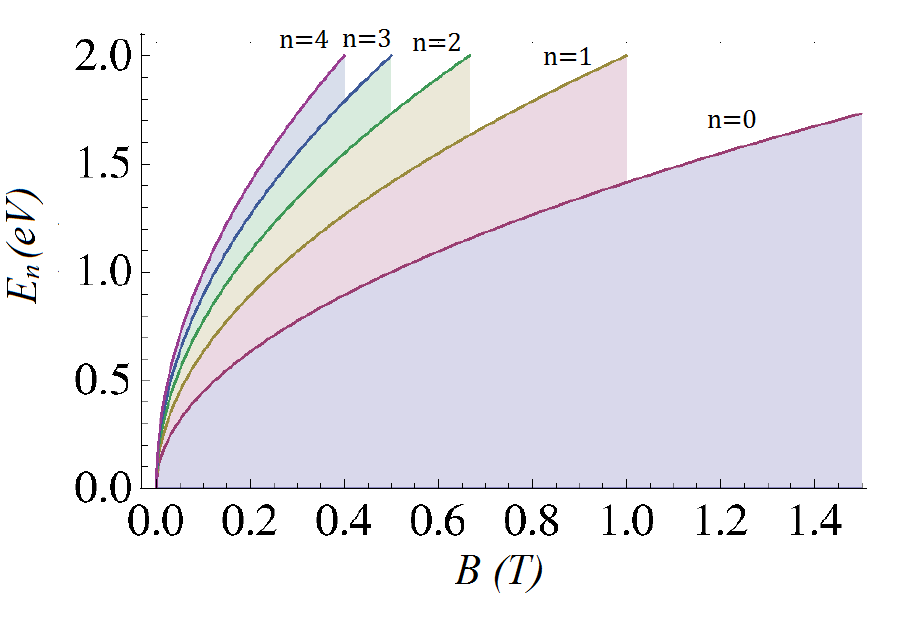
\includegraphics[width=0.5\linewidth]{img/figure_7}
  \captionof{figure}{\emph{Abanico de Dirac-Landau. Representación de los posibles valores de energía de los electrones, en el problema de Dirac-Landau en el plano, según el valor del campo magnético} [11].} \label{fig:Abanico Dirac}
\end{figure}
Como vemos, al igual que en el problema de Landau, la restricción al plano del problema da lugar a unos niveles energéticos cuantizados en función de un único número cuántico, $n$. Esta energía depende también únicamente del campo magnético, solo que ahora no es de manera lineal, como podemos ver en la Figura \ref{fig:Abanico Dirac}.








\newpage
\leavevmode\thispagestyle{empty}\newpage



%%%%%%%%%%%%%%%%%%%%%%%%%%%%%%%%%%%%%%%%%%%%%
\section{Aplicaciones}
%%%%%%%%%%%%%%%%%%%%%%%%%%%%%%%%%%%%%%%%%%%%%







%%%%%%%%%%%%%%%%%%%%%%%%%%%%%%%%%%%%%%%%%%%%%
\subsection{El efecto Hall cuántico: Problema de Landau}
%%%%%%%%%%%%%%%%%%%%%%%%%%%%%%%%%%%%%%%%%%%%%









$$\\$$%%%%%%%%%%%%%%%%%%%%%%%%%%%%%%%%%%%%%%%%%%
\textbf{Efecto Hall Clásico}
$$\\$$%%%%%%%%%%%%%%%%%%%%%%%%%%%%%%%%%%%%%%%%%%









El efecto Hall es como se denomina al fenómeno por el cual aparece un campo eléctrico en un material cuando por él circula una corriente y se le aplica un campo magnético perpendicular a esta. El campo eléctrico generado es perpendicular a la corriente y al campo magnético simultaneamente. Su origen es debido a la reorganización espacial de las cargas dentro del conductor por la presencia del campo magnético. $$\\$$
Este efecto fue observado por primera vez en 1880 por el físico estadounidense Edwin Herbert Hall, cuando estudiaba el comportamiento de una corriente en una lámina conductora muy delgada de grosor $\delta$, en presencia de un campo magnético [12]. $$\\$$
Cuando sometemos a un conductor (o semiconductor) por el que circula una corriente, $\vec{j}$, a un campo magnético, $\vec{B}$,  perpendicular a esta, los portadores experimentan una fuerza perpendicular a la corriente y al campo simultaneamente, debido a la fuerza de Lorentz (\ref{Fuerza de Lorentz}). $$\\$$
\begin{equation*}
\vec{F} = q (\vec{E} + \frac{\vec{v}}{c}\wedge \vec{B}) \qquad.
\end{equation*} $$\\$$
El sentido de la fuerza depende del signo de los portadores, por lo que se produce una reorganización de las cargas dentro del material. Esta nueva distribución hace que haya un gradiente de potencial en la dirección de la fuerza y, por consiguiente, que aparezca un campo eléctrico en la misma dirección que la fuerza, pero sentido contrario. $$\\$$
En el caso de un una lámina muy delgada situada en el plano $X_1X_2$, y sometida a un campo magnético de la forma, $\vec{B}=B\vec{e}_3$, en el que circula una corriente en la dirección $X_1$ como el mostrado en la Figura \ref{fig:Hall clasico}, la fuerza que experimentan los portadores debida al campo magnético es $$\\$$
\begin{equation*}
\vec{F} = q \frac{v}{c} B \vec{e}_2 \qquad.
\end{equation*} $$\\$$
De modo que el campo eléctrico que aparece dentro del conductor en el equilibrio, cuando la fuerza eléctrica que experimentan los portadores contrarresta la fuerza debida al campo magnético externo es $$\\$$
\begin{equation*}
\vec{E} = - q \frac{v}{c}B \vec{e}_2 \qquad.
\end{equation*} $$\\$$
Por medio de la ley de Ohm tenemos que  $$\\$$ 
\begin{equation*}
\vec{j} = \sigma_o \left( \vec{E} + \frac{1}{c} \vec{v} \wedge \vec{B}\right) = \sigma_o \left( \vec{E} + \frac{1}{nqc} \vec{j} \wedge \vec{B}\right) \qquad ,
\end{equation*} $$\\$$
donde hemos utilizado que $\vec{j}=qn\vec{v}$ siendo $n$ la densidad de portadores y $\sigma_o$ la conductividad del vacío. Esto nos lleva a una relación lineal entre la corriente y el campo eléctrico, $\vec{j} = \rho \vec{E}$, [13] por medio de una ecuación matricial, la cual nos da el el tensor de resistividad [17]. $$\\$$
\begin{equation*}
\rho = \begin{pmatrix} \rho_{xx} & \rho_{xy} \\ \rho_{yx} & \rho_{yy} \end{pmatrix} = 
\begin{pmatrix} \rho_{o} & -\frac{B}{nqc} \\ \frac{B}{nqc} & \rho_{o} \end{pmatrix} \qquad .
\end{equation*} $$\\$$
Se define la resistencia Hall como [31] $$\\$$
\begin{equation}
R_H = \frac{\rho_{xy}}{\delta} = \frac{B}{n|q|c \delta} \qquad .
\end{equation} $$\\$$
Una de las principales aplicaciones del efecto Hall, consiste en determinar la densidad de carga de los portadores de un semiconductor (electrones o huecos), en función del valor de la resistencia Hall. $$\\$$
\begin{equation*} 
n = \frac{B}{R_H |q| c \delta} \qquad .
\end{equation*} $$\\$$
\begin{figure}
  \centering
  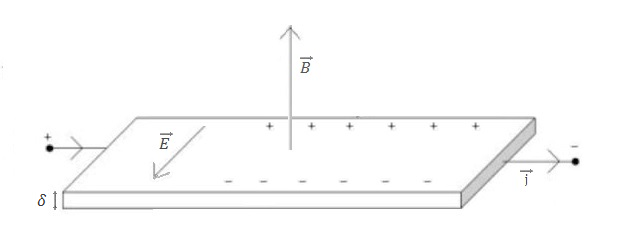
\includegraphics[width=0.6\linewidth]{img/figure_8}
  \captionof{figure}{\emph{Efecto Hall Clásico en una lámina conductora.}} \label{fig:Hall clasico}
\end{figure}






$$\\$$%%%%%%%%%%%%%%%%%%%%%%%%%%%%%%%%%%%%%%%%%%
\textbf{Efecto Hall Cuántico}
$$\\$$%%%%%%%%%%%%%%%%%%%%%%%%%%%%%%%%%%%%%%%%%%








Al intentar estudiar el Efecto Hall clásico bajo diferetens condiciones, se descubrió de manera inesperada el Efecto Hall Cuántico, que es un fenómeno totalmente diferente y que es puramente cuántico. Este efecto consiste en la cuantización de la conductividad, $\sigma=\rho^{-1}$, de un material en presencia de un campo magnético externo muy intenso. Para electrones, $q=-e$, $e>0$ la conductividad es $$\\$$
\begin{equation*}
\sigma = \begin{pmatrix} \sigma^{xx} & \sigma^{xy} \\ \sigma^{yx} & \sigma^{yy} \end{pmatrix} = \begin{pmatrix} 0 & -i\frac{e^2}{h} \\ i\frac{e^2}{h} & 0 \end{pmatrix} \hspace{2cm} i = 1,2,3,... \qquad .
\end{equation*} $$\\$$
La conductividad longitudinal, $\sigma^{xx}$ y $\sigma^{yy}$, se anula, mientras que la transversal, $\sigma^{xy}$ y $\sigma^{yx}$, está cuantizada. De forma general vamos a referirnos por conductividad a la conductividad transversal, viene dada por: $$\\$$
\begin{equation}
\sigma^{xy} = \pm i\frac{e^2}{h} \hspace{2cm} i = 1,2,3,...
\end{equation} $$\\$$
Este efecto fue predicho por Ando, Matsumoto y Uemure en 1975 [14], y posteriormente medido por Klaus von Klitzing en 1980, que sometiendo laminas de un material semiconductor, con un grosor mucho menor que las que usó Hall en su experimento ($\delta \rightarrow 0$), a campos magnéticos muy intensos ($15 \; T$) a temperaturas muy bajas ($2 \; K$) [15]. En este experimento se observó que la resistencia Hall no dependía linealmente del campo magnético si no que permanecía constante en determinados intervalos de este, tras los que crecía a otro valor superior, mostrando un comportamiento escalonado. $$\\$$
\begin{figure}
  \centering
  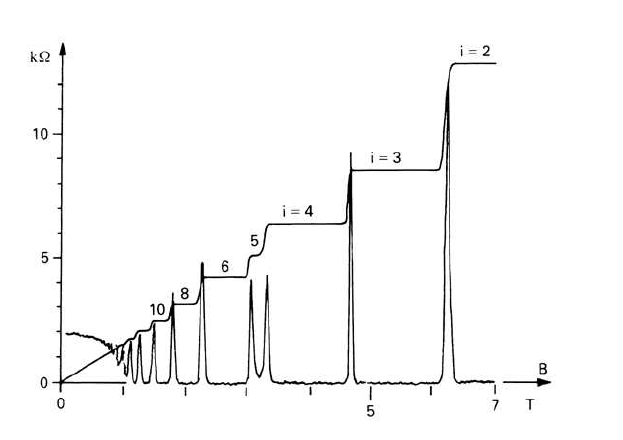
\includegraphics[width=0.5\linewidth]{img/figure_9}
  \captionof{figure}{\emph{Efecto Hall Cuántico Entero. Medida de $R_H$ en función del campo magnético }[16].} \label{fig:Efecto hall cuantico entero}
\end{figure}
\begin{equation}
R_H = \frac{h}{ E^2 i} \hspace{2cm} i = 1,2,3,...
\end{equation} $$\\$$
La explicación de este hecho se fundamenta en la estructura de niveles del problema de Landau. Para entenderlo tenemos que definir la densidad de estados de los niveles de Landau, que depende del número de estados degenerados por cada nivel [31]$$\\$$
\begin{equation*}
n_B =\frac{n^\circ \; de \;  estados}{L_1 L_2} = \frac{e B}{hc} \qquad . 
\end{equation*} $$\\$$
Para un determinado número de portadores atravesando un material, los primeros $n_B$ llenarán el nivel fundamental, $i=0$, luego el primer estado excitado, $i=1$ y así sucesivamente (usamos $i$ para designar los niveles para no confundirlo con la densidad de portadores, $n$). Teniendo en cuenta que $n_B$ depende de la intensidad de campo magnético, $B$, el número de niveles ocupados cambia en función de este. La conductividad del material depende del número de niveles de Landau ocupados por los portadores, por tanto, permanece constante hasta que el valor del campo magnético crece lo suficiente como para que $n_B$ sea lo suficientemente grande como para poder albergar todos los portadores con menos niveles.  $$\\$$
La importancia de este fenómeno radica en que hasta la fecha se pensaba que la resistencia y la conducción en un material dependían únicamente de factores geométricos y de parámetros intrínsecos del material, como la conductividad. En lugar de esto, se vio que la conductividad puede depender del campo magnético aplicado en materiales semiconductores, dando lugar a diferentes mesetas con valor constante para diferentes valores del campo magnético. Por otro lado también es notorio la presencia de un efecto puramente cuántico a nivel macroscópico [17]. $$\\$$
Una de las aplicaciones de este experimento es la medición de la constante de estructura fina expresándola en términos de la resistencia Hall [15]. $$\\$$
\begin{equation}
\alpha = \frac{\mu_0 c e^2}{2 h} = \frac{\mu_0 c }{2 i R_H} \hspace{2cm} i=1,2,3,...\qquad,
\end{equation} $$\\$$
siendo $\mu_0$ es la permeabilidad del vacío y $i$ el factor de llenado $$\\$$
\begin{equation}
i= \left.\frac{n}{n_B} \right|_\mathbb{Z} \qquad .
\end{equation} $$\\$$
\begin{figure}
  \centering
  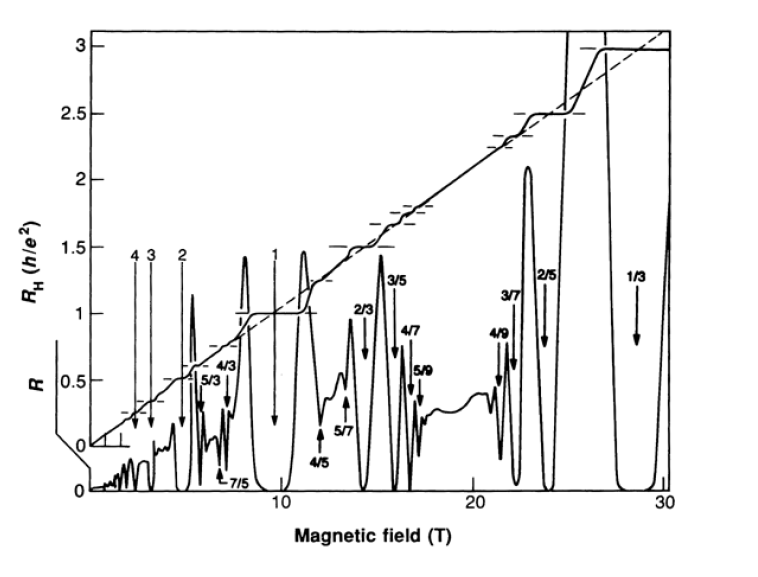
\includegraphics[width=0.5\linewidth]{img/figure_10}
  \captionof{figure}{\emph{Efecto Hall Cuántico Fraccionario} [16].} \label{fig:Efecto hall cuantico entero}
\end{figure}
Posteriormente en 1982, Tsui, Stormer y Gossard, utilizando diferentes materiales, encontraron este mismo efecto  para valores fraccionarios del factor de llenado, o lo que es lo mismo, no había un salto en la resistividad cada vez que se vaciaba un nivel, si no también cuando se vaciaban parcialmente [18]. Este suceso se denomina Efecto Hall Cuántico Fraccionario y su explicación conceptual es más difícil que la del Efecto Hall Cuántico Entero. Los valores de los posibles números fracionarios no son cualquiera, si no que solo se observó primeramente el de $f=1/3$, y posteriormente otros como $f=2/5$, $1/5$, ... $$\\$$
El Efecto Hall Cuántico Fraccionario no puede explicarse tratando a los electrones como si fuesen libres, si no que requiere tener en cuenta la interacción entre estos. Hemos visto que el Efecto Hall Cuántico Entero era debido a la degeneración de los niveles, pero teniendo en cuenta la interacción entre electrones los niveles, así como su degeneración, cambian. La forma de interpretar el significado de los valores fraccionarios es pensando que una fracción de la carga de los electrones pertenece a un nivel energético mientras que otra fracción a otro. Esta interpretación es meramente conceptual puesto que los electrones son partículas indivisibles [17][19]. 










$$\\$$%%%%%%%%%%%%%%%%%%%%%%%%%%%%%%%%%%%%%%%%%%%%%
\subsection{El Grafeno: Problema de Dirac-Landau}
$$\\$$%%%%%%%%%%%%%%%%%%%%%%%%%%%%%%%%%%%%%%%%%%%%%










El Grafeno es un compuesto cristalino, formado por átomos de carbono en una red hexagonal bidimensional. Su popularidad en estos últimos años es debido a sus peculiares propiedades que le hacen muy interesante tanto desde el punto de  vista electrónico como mecánico. La diferencia con el grafito es que este hace referencia a una red tridimensional, mientras que el Grafeno es un cristal bidimensional, lo cual es lo que le confiere propiedades muy interesantes. $$\\$$
\begin{figure}
  \centering
  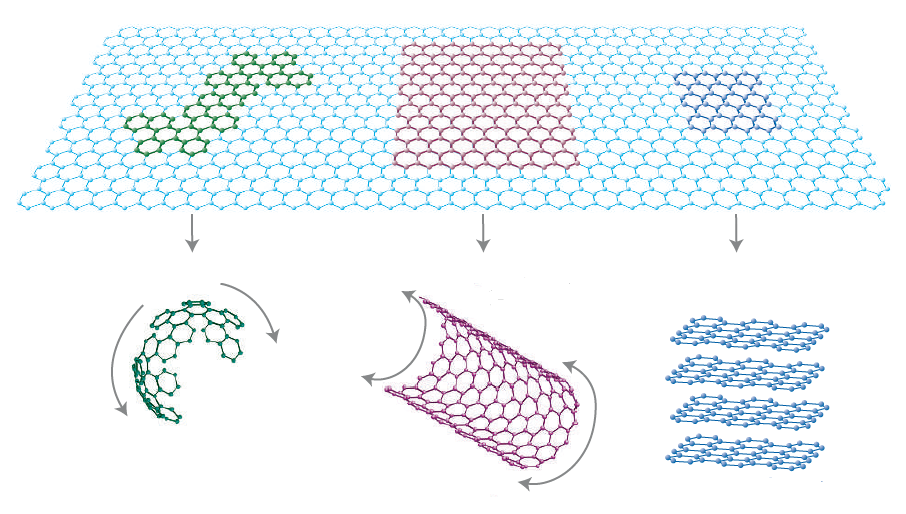
\includegraphics[width=0.5\linewidth]{img/figure_11}
  \captionof{figure}{\emph{Estructura cristalina del Grafeno, red plana hexagona. Puede dar lugar a diferentes estructuras envolviendose sobre sí misma o apilandose en capas (grafito)} [21].} \label{fig:Grafeno}
\end{figure}
Desde la Electrodinámica Cuántica el Grafeno destaca entre otros cristales bidimensionales por diferentes motivos. Por un lado la movilidad de sus portadores puede exceder valores de $15000 cm^2V^{-1}s^{-1}$ para concentraciones de $n=10^{12} cm^{-2}$ tanto si es dopado eléctrica o químicamente y además, dependiendo débilmente de la temperatura [21]. Este hecho es debido a su alta temperatura de Debye, que impide el scattering de fotones, así como también a su estructura de bandas en torno a la posición $\Gamma$ de la primera zona de Brillouin. Otra cualidad destacable desde la Electrodinámica Cuántica es que en el Grafeno, el Efecto Hall Cuántico (Efecto Hall Cuántico) es apreciable a temperatura ambiente [28]. $$\\$$
Desde el punto de vista teórico, en la física de la materia condensada se suele interpretar a los portadores como partículas semiclásicas descritas por la ecuación de Schroedinger. En cambio, el hecho de que el Grafeno sea una red bidimensional y que las bandas energéticas nos den una velocidad de Fermi, $v_F$, prácticamente constante hasta energías no muy altas ($|E|<1eV$), hace que la descripción de los portadores sea más exacta por medio de la ecuación de Dirac en (2+1)-dimensiones sin masa, o ecuación de Weyl, con una velocidad de efectiva de $v_F=10^6 ms^{-1}$ [28]. Otras propiedades que influyen en el éxito de esta descripción son que el gap entre la banda de valencia y la de conducción sea prácticamente nulo y que el momento sea independiente de la velocidad de Fermi. $$\\$$
Teniendo en cuenta estas consideraciones, se puede demostrar que podemos describir el comportamiento de los electrones en el Grafeno por medio del Hamiltoniano: [21] $$\\$$
\begin{equation} \label{Hamiltoniano Grafeno}
H = \begin{pmatrix} 0 & v_F(ip_1 \pm p_2) \\ v_F(ip_1 \mp p_2) & 0 \end{pmatrix} = v_F (\sigma^1 p_1 \pm \sigma^2 p_2) \qquad .
\end{equation} $$\\$$
Es importante enfatizar que esta descripción es debida a las simetrías del cristal, ya que las bandas energéticas de las dos subredes que constituyen la red bidimensional, tienen un comportamiento cosenoidal y que se intersectan en cero en los límites de la zona de Brillouin. Además, para $|E|<1eV$, este comportamiento se caracteriza con un espectro cónico, y por lo tanto una energía lineal con el momento. $$\\$$
\begin{figure}
  \centering
  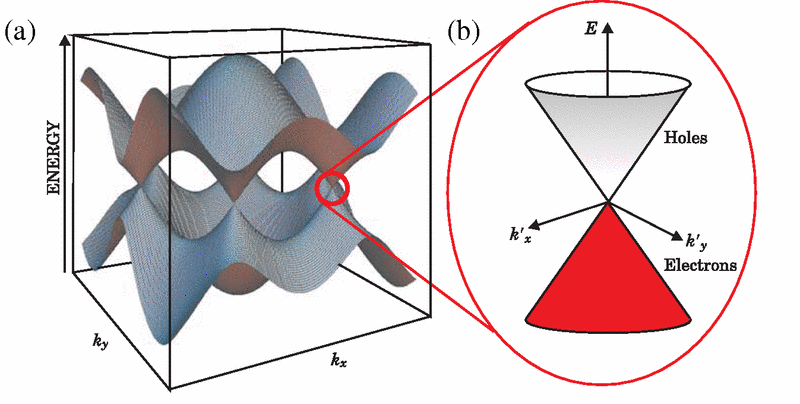
\includegraphics[width=0.5\linewidth]{img/figure_12}
  \captionof{figure}{\emph{Estructura de bandas del Grafeno. Se puede ver que el gap entre la banda de valencia y conducción es prácticamente nula, y que para $|E|<1eV$ tiene un comportamiento cónico} [33].} \label{fig:bandas Grafeno}
\end{figure}
\begin{equation}
E = \pm v_F |\vec{p}| \qquad .
\end{equation} $$\\$$
Otra importante característica de este resultado es que los electrones en el Grafeno, se describen por medio de espinores de dos componentes, pero el significado de las componentes no es el mismo que en el caso de los espinores de Dirac de partícula libre. Cada estado electrónico se obtiene como combinación de estados propios de cada una de las dos subredes que forman en cristal, de esta forma, cada componente del espinor es la contricubión de cada red al estado y no la contribución del espín usual de la Electrodinámica Cuántica (que se puede añadir posteriormente). Esto es característico del Grafeno y se denomina \textit{pseudospín}. Las matrices $\sigma^i$ en (\ref{Hamiltoniano Grafeno}) hacen referencia al pseudospín [21]. $$\\$$
El hecho de que la velocidad de la luz efectiva del Hamiltoniano (\ref{Hamiltoniano Grafeno}) sea 300 veces menor que $c$, hace que todos los resultados relativistas propios de la ecuación de Dirac en el plano sean más visibles en el Grafeno. Del mismo modo, por este mismo motivo, el pseudoespín tiene un papel más importante para la descripción de los electrones en el Grafeno que el espín real. $$\\$$
En analogía con la Electrodinámica Cuántica podemos definir la quiralidad de partículas no masivas por medio de la helicidad, la proyección de $\vec{\sigma}=(\sigma^1,\sigma^2)$ en la dirección del momento $\vec{p}$. La quiralidad en el Grafeno, nos permite relacionar los estados de electrones con momento $\vec{p}$ con los de los huecos con momento $-\vec{p}$.











$$\\$$%%%%%%%%%%%%%%%%%%%%%%%%%%%%%%%%%%%%%%%%%%%%%%%%%%
\textbf{Efecto Hall Cuántico en el Grafeno}
$$\\$$%%%%%%%%%%%%%%%%%%%%%%%%%%%%%%%%%%%%%%%%%%%%%%%%%%









Entre todas las propiedades dentro de la Electrodinámica Cuántica del Grafeno, hemos visto, que destaca el hecho de que se observa el Efecto Hall Cuántico a temperatura ambiente debido a que en el Grafeno los electrones y huecos, en vez de estar descritos como partículas semiclásicas, siguen un comportamiento análogo a partículas de Dirac sin masa. De todos los experimentos realizados se ha observado la aparición del Efecto Hall Cuántico de dos maneras distintas. $$\\$$
\begin{figure}
  \centering
  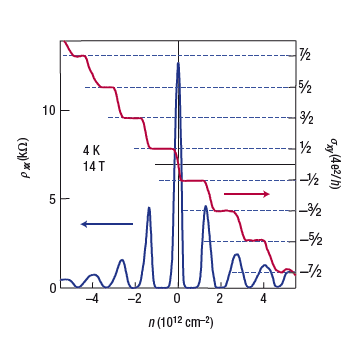
\includegraphics[width=0.4\linewidth]{img/figure_13}
  \captionof{figure}{\emph{Efecto Hall Cuántico Entero en el Grafeno, donde se observa un desplazamiento de 1/2} [21].} 
\end{figure}
Para muestras de una sola capa se ha observado un análogo al Efecto Hall Cuántico entero, que, aunque no es un fenómeno diferente, tampoco es el Efecto Hall Cuántico entero convencional. En estas muestras se ha visto una conductividad transversal $\sigma^{xy}$ con un comportamiento escalonado de la forma $$\\$$
\begin{equation}
\sigma^{xy} = \pm 4 \frac{e^2}{h}\left(i + \frac{1}{2} \right) \qquad ,
\end{equation} $$\\$$
donde $i$ hace referencia al nivel Landau de los portadores. Se parece a la expresión que vimos para el Efecto Hall Cuántico Entero, a diferencia de un factor 4, debido a la degeneración de spín y de  carga, y un desplazamiento de 1/2, que es debido a la existencia de un nivel cuántico compartido para electrones y huecos a $E=0$, lo cual puede interpretar matemáticamente como una causa del acoplamiento del momento angular con el pseudospín. $$\\$$
La energía de los niveles de Dirac-Landau es $$\\$$
\begin{equation}
E = \pm v_F \sqrt{2\hbar \frac{eB}{c} i} \qquad . 
\end{equation} $$\\$$
Por otro lado, para muestras de Grafeno bicapa se observa un fenómeno similar, donde ahora la conductividad transversal viene dada por $$\\$$
\begin{equation}
\sigma^{xy} = \pm 4 \frac{e^2}{h}i \qquad ,
\end{equation} $$\\$$
donde no tenemos el desplazamiento de 1/2 que teníamos con muestras de una capa. Otra diferencia es que experimentalmente no se mide ningún escalón para $i=0$, lo cual nos dice que el Grafeno tiene un comportamiento metálico en ese punto. Esto es debido a que para muestras bicapa, es más exacto describir los portadores por medio del Hamiltoniano $$\\$$
\begin{equation} 
H = \frac{1}{2m^*} \begin{pmatrix} 0 & (ip_1 - p_2)^2 \\ (ip_1+p_2)^2 & 0 \end{pmatrix} \qquad .
\end{equation} $$\\$$
Este tiene la estructura no diagonal propia de la ecuación de Dirac sin masa, pero con los términos cinéticos propios del Hamiltoniano de Schroedinger, con una masa efectiva $m^* = 0.05 m_e$. En este caso los niveles de Landau vienen dados por $$\\$$
\begin{equation}
E = \hbar \omega_c \sqrt{i(i-1)} \qquad ,
\end{equation} $$\\$$
\begin{figure}
  \centering
  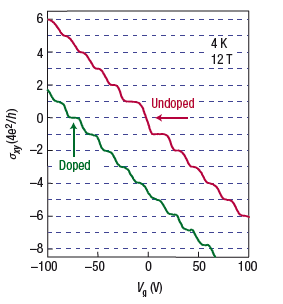
\includegraphics[width=0.35\linewidth]{img/figure_14}
  \captionof{figure}{\emph{Efecto Hall Cuántico Entero en una muestra bicapa del Grafeno. En rojo muestra sin dopar, en verde dopado} [21].} 
\end{figure}
donde $\omega_c$ es la frecuencia ciclotrón. Vemos que los niveles $i=0$ e $i=1$ están degenerados, lo cual es lo que produce que desaparezca el escalón a $i=0$ experimentalmente. La falta de existencia de una meseta para $i=0$ se puede evitar dopando el cristal con impurezas donadoras. \newpage





\leavevmode\thispagestyle{empty}\newpage


$$\\$$%%%%%%%%%%%%%%%%%%%%%%%%%%%%%%%%%%%%%%%%
\section{Conclusiones}
%%%%%%%%%%%%%%%%%%%%%%%%%%%%%%%%%%%%%%%%









Las conslusiones y resultados obtenidos en este trabajo son las siguientes: $$\\$$
\begin{changemargin}{0.75cm}{0cm} 
\begin{enumerate}
\item Hemos resuelto el problema del movimiento de fermiones en campos magnéticos constantes satisfactoriamente en diferentes estadios: clásico, cuántico y cuántico-relativista tanto en $\mathbb{R}^3$ como en $\mathbb{R}^2$. De este modo, hemos visto tanto que tienen en común la solución de oscilador, como las peculiaridades propias de cada uno. $$\\$$
\item El movimiento de los fermiones sometidos a un campo magnético constante en el caso clásico es independiente de la elección del gauge que se tome para el campo magnético, sin embargo en el caso cuántico relativista (problema de Dirac-Landau) y no-relativista (problema de Lnadau) las autofunciones que se obtienen sí que depende de la elección de gauge. $$\\$$
En el gauge simétrico obtenemos soluciones con simetría bajo rotaciones en el plano $X_1X_2$, mientras que en el gauge de Landau estas son invariantes bajo translaciones en la dirección $\vec{e}_1$, sin embargo, este hecho no afecta al espectro ni a los observables, los cuales son independientes de la elección del mismo. $$\\$$
\item La restricción al plano del movimiento de partículas cargadas en presencia, o no, de un campo magnético, no supone más que una reducción de los grados de libertad tanto para el estudio clásico como cuántico. Para el problema cuántico-relativista, definido por la ecuación de Dirac, supone un cambio más profundo. $$\\$$
En la restricción al plano de la ecuación de Dirac, pasamos de una ecuación matricial de rango 4, a una de rango 2. Esto hace que tengamos que escoger entre dos representaciones no equivalentes para las matrices $\alpha^i$ y $\beta$, para poder obtener las soluciones físicas posibles. $$\\$$
\item Comprobamos que en el límite no-relativista de la ecuación de Dirac acoplada a un campo magnético, llegamos a la ecuación de Pauli en presencia de un campo magnético donde aparace el término de acoplamiento del espín con el campo magnético de forma natural y el valor correcto del factor giromagnético para los electrones. Además hemos obtenido otros términos que constituyen las correcciones relativistas de la ecuación de Schroedinger. $$\\$$
\item Hemos visto que la descripción matemática del movimiento de fermiones en campos magnéticos desde un punto de vista cuántico-relativista, tiene interés más allá del ámbito teórico, siendo necesaria para describir fenómenos como el Efecto Hall Cuántico entero así como el comportamiento de los electrones en el Grafeno, debido a su peculiar estructura cristalina, en particular. $$\\$$ $$\\$$
\end{enumerate}
\end{changemargin}
$$\\$$%%%%%%%%%%%%%%%%%%%%%%%%%%%%%%%%%%%%%%%%
\section*{Conclusions}
%%%%%%%%%%%%%%%%%%%%%%%%%%%%%%%%%%%%%%%%
The conclusions and results which have been in this study are: $$\\$$
\begin{changemargin}{0.75cm}{0cm} 
\begin{enumerate}
%Hemos resuelto el problema del movimiento de fermiones en campos magnéticos constantes satisfactoriamente en diferentes estadios: clásico, cuántico y cuántico-relativista tanto en $\mathbb{R}^3$ como en $\mathbb{R}^2$. De este modo, hemos visto tanto que tienen en común la solución de oscilador, como las peculiaridades propias de cada uno.
\item  We have solved the problem of the movement of fermions in a magnetic constant field properly in different frames: classical, quantum and quantum-relativistic in $\mathbb{R}^3$ and in $\mathbb{R}^2$. Consequently we have seen that they have in common the oscillator solution, as well as the owned peculiarities by each one.$$\\$$
%\item El movimiento de los fermiones sometidos a un campo magnético constante en el caso clásico es independiente de la elección del gauge que se tome para el campo magnético, sin embargo en el caso cuántico relativista (problema de Dirac-Landau) y no-relativista (problema de Lnadau) las autofunciones que se obtienen sí que depende de la elección de gauge. $$\\$$
%En el gauge simétrico obtenemos soluciones con simetría bajo rotaciones en el plano $X_1X_2$, mientras que en el gauge de Landau estas son invariantes bajo translaciones en la dirección $\vec{e}_1$, sin embargo, este hecho no afecta al espectro ni a los observables, los cuales son independientes de la elección del mismo. $$\\$$
\item  The movement of fermions subjected to a constant magnetic field, from a classical view, is independent  of the choice of gauge made to describe the magnetic field, in contrast, in the quantum non-relativistic (problem of Dirac-Landau) and relativistic problem (problem of Landau) the eigenstates obtained depend on the choice of gauge. $$\\$$ 
In the symmetrical gauge we get solucion with simmetry under rotations in the plane $X_1X_2$, whilst in the gauge of Landau, this solutions are invariant under translations in the direction $\vec{e}_1$, however, this fact does not affect either the spectre or any observable, which are independent of the choice of the representation.$$\\$$
%\item La restricción al plano del movimiento de partícular en presencia, o no, de un campo magnético, no supone más que una reducción de los grados de libertad tanto para en el estudio clásico como cuántico. Para el problema cuántico-relativista, definido por la ecuación de Dirac, supone un cambio en la forma en la que se presentan las ecuaciones para obtener las soluciones. $$\\$$
\item The constraint to the plane of the movement of charged particles in presence, or not, of a megnetic field, yields no more than a reduction of the degrees of freedom in the classical study as well as in the quantum study. The quantum-relativistic problem, defined by the equation of Dirac-Landau, implies a deeper change. $$\\$$
%Con la restricción al plano de la ecuación de Dirac, pasamos de un problema matricial de rango 4, a uno de rango 2. Esto hace que tengamos que escoger dos representaciones no equivalentes para los coeficientes $\alpha^i$ y $\beta$, para poder obtener una descripción de todas las soluciones físicas posibles. $$\\$$
In the constraint to the plain in the equation of Dirac, we move from a matricial equation of range 4 to another one of range 2. This force us to choose between two unequivalent representations for the matrixes $\alpha^i$ and $\beta$ in order to achieve a description of all the possible physical solutions. $$\\$$
%\item Comprobamos que en el límite no-relativista del problema de Dirac, con el acoplamiento del cuadripotencial vector con el cuatrimomento, recuperamos la ecuación de Schroedinger en presencia de un campo magnético con el término de acoplamiento del espín con el campo magnético de forma natural y el valor correcto del factor giromagnético para los electrones. Además hemos obtenido otros términos que constituyen correcciones relativista de la ecuación de Schroedinger. $$\\$$
\item We make sure that the non-relativistic limit of the equation of Dirac, coupled to a magnetic field, we recover the equation of Pauli in presence of a magnetic field where appears the term of coupling between the spin and the magnetic field naturally and the correct value of the giromagnetic factor for electrons. Besides we have obtained other term that show relativistic corrections on the equation of Schroedinger. $$\\$$ 
%\item Hemos visto que la descripción matemáticas del movimiento de fermiones en campos magnéticos desde un punto de vista cuántico-relativista, tiene interés más allá del ámbito teórico, siendo necesaria para describir fenómenos como el efecto Hall cuántico en general, como el comportamiento de electrones dentro del Grafeno, debido a su peculiar estructura cristalina, en particular. $$\\$$ $$\\$$
\item We have present that the mathematical description of the movement of fermions in magnetic fields in a quantum-relativistic frame, possess interest beyond the theorical ambit, being it necessary to explain phenomenoes such as the Quantum Hall Effect in general, and the behaviour of electrons in the Graphene, due to its peculiar crystal estructure, in particular.
\end{enumerate}
\end{changemargin}
\newpage



\leavevmode\thispagestyle{empty}\newpage



%%%%%%%%%%%%%%
\section{Bibliografía}
%%%%%%%%%%%%%%




[1] GREINER, W. \emph{Relativistic Quantum Mechanics Wave Equations}. Springer, 2000. \\

[2] SAKURAI, J.J.  \emph{Advanced Quantum Mechanics}. 1967. \\

[3] BETHE, H.A., JACKIW, R. \emph{Intermediate Quantum Mechanics}. Advanced Book Classics, 1997.\\

[4] LANDAU, L.D., LIFSHITZ, E.M. \emph{Course of Theorical Physics Vol. 3. Quantum Mechanics Non-relativistic Theory}. Pergamon Press, 1977. \\

[5] DIRAC, P.A.M. \emph{The quantum theory of the electron}. St. John's College, Cambridge, 1928. \\

[6] SCHROEDINGER, E. \emph{An Undulatory Theory of the Mechanics of Atoms and Molecules}. Physical Review, 1926. \\

[7] HERNANDEZ ORTIZ, S.F. \emph{Mapeo a una Mecánica Cuántica SUSY para la
ecuación de Dirac en el plano}. Instituto de Física y Matemáticas, Universidad Michoacana, 2008. \\

[8] BASHIR, A., ANGUIANO GALICIA, M.J. \emph{Fermions in odd space-time dimensions:
back to basics}. 2011. \\

[9] MCDONALD, K.T. \emph{Electrodynamics in 1 and 2 Spatial Dimensions}. Joseph Henry Laboratories, Princeton University, 2014. \\

[10] ABRAMOWITZ, M., STEGUN, I. \emph{Handbook of Mathematical Functions}. National Bureau of Standards, 1972. \\

[11] GONZALEZ VALDÉS, J.M. \emph{Electrones planares en un campo magnético}. Universidad Michoacana de San Nicolás de Hidalgo, 2012. \\

[12] HALL, E. \emph{On a New Action of the Magnet on Electric Currents}. American Journal of Mathematics, 1879. \\

[13] GRIFFITHS, D.J. \emph{Introduccion to electrodynamics}. Prentice Hall, 1999. \\

[14] ANDO, T., MATSUMOTO, Y., UEMURA, Y. \emph{Theory of Hall Effect in a Two-Dimensional Electron System}. Journal of the Physical Society of Japan, 1975. \\

[15] KLITZING, K., DORDA, G., PEPPER, M. \emph{New Method for High-Accuracy Determination of the Fine-Structure Constant Based on Quantized Hall Resistance}. Physical Review Letters, 1980. \\

[16] LAUGHLIN, R. B. \emph{Quantized Hall conductivity in two dimensions}. Physical Review B, 1981. \\

[17] TONG, D. \emph{The Quantum Hall Effect}. TIFR Infosys Lectures, 2016. \\

[18] TSUI, D.C., STORMER, H.L., GOSSARD, A.C. \emph{Two-Dimensional Magnetotransport in the Extreme Quantum Limit}. Physical Review Letters, 1982. \\

[19] STORMER, H.L. \emph{Nobel Lecture: The fractional quantum Hall effect}. Reviews of Modern Physics, 1999. \\

[20] LAUGHLIN \emph{Anomalous Quantum Hall Effect: An Incompressible Quantum Fluid with Fractionally Charged Excitations}. Physical Review Letters, 1983. \\

[21] GEIM, A.K., NOVOSELOV, K.S. \emph{The rise of Graphene}. Nature Materials, 2007. \\

[22] BRODIE, B. C. \emph{On the Atomic Weight of Graphite}. Philosophical Transactions of the Royal Society of London, 1859. \\

[23] WALLACE, P.R. \emph{The Band Theory of Graphite}. Physical Review, 1947. \\

[24] SEMENOFF, G. W. \emph{Condensed-Matter Simulation of a Three-Dimensional Anomaly}. Physical Review Letters, 1984. \\

[25] RUESS, G.; VOGT, F. \emph{CHöchstlamellarer Kohlenstoff aus Graphitoxyhydroxyd}. Monatshefte für Chemie, 1948. \\

[26] NOVOSELOV, K. S., GEIM, A. K., MOROVOZ, S. V., JIANG, D., KATSNELSON, M. I., GRIGORIEVA, I. V., DUBONOS, S. V., FIRSOV, A. A.  \emph{Two-dimensional gas of massless Dirac fermions in Graphene}. Nature, 2005. \\

[27] ZHANG, Y., TAN, Y. W., STORMER, H. L.; KIM, P \emph{Experimental observation of the quantum Hall effect and Berry's phase in Graphene}. Nature, 2005. \\

[28] NOVOSELOV, K. S., GEIM, A. K., MOROVOZ, S. V., JIANG, D.; ZHANG, Y., GRIGORIEVA, I. V., DUBONOS, S. V., FIRSOV, A. A. \emph{Electric Field Effect in Atomically Thin Carbon Films}. Science, 2004. \\

[28] NOVOSELOV, K. S., GEIM, A. K., MOROVOZ, S. V., JIANG, D.; ZHANG, Y., STORMER, H.L., MAAN, J.C., BOEBINGER, C.S., KIM, P.\emph{Room-Temperature Quantum Hall Effect in Graphene}. Science, 2007. \\

[29] KEHREIN, S., FARIBAULT, A. \emph{Problem Set 03 Landau Levels}. Mesoscopic Physics, 2011. \\

[30] KOSMAS, O.T. \emph{Charged Particle in an Electromagnetic Field Using Variational Integrators}. University of Erlangen-Nuremberg, 2011. \\

[31] DE LA TORRE MAYADO, M. \emph{Electrodinámica Cuántica Bidimensional: Sobre
la Teoría del Efecto Hall Cuántico}. Departamento de Física, Ingeniería y Radiología Médica Universidad de Salamanca. \\

[32] BITTENCOURT J.A., \emph{Fundamentals of plasma physics}. Springer, 2004. \\

[33] DAS SARMA, S., ADAM, S., HWANG, E.H., ROSSI, E. \emph{Electronic transport in two dimensional Graphene}. Review of modern physics, 2010. \\





%\addcontentsline{toc}{section}{References}
%\begin{thebibliography}{}


%\bibitem[1]{Hermoso} \emph{Amplificador Operacional}. 
%Extraido el 11 de marzo del 2015 de
%http://www.uhu.es/adoracion.hermoso/Documentos/Tema-4-AmpliOperc.pdf

%\bibitem[2]{Texas Instruments}  \emph{LM741 Operational Amplifier}. Extraído el 11 de marzo del 2015 de

%\bibitem[3]{Cascante} \emph{Guía de Laboratorio Electrico II}. Universidad de Costa Rica, Escuela de Ingeniería Eléctrica



%\bibitem[4]{embedded} embedded. \emph{Typically typical}. Recuperado el 11 de marzo del 2015 de: $http://www.embedded.com/electronics-blogs/break-points/4418969/Typically-typical$


%\bibitem[5]{UNAL} Universidad Nacional de Colombia. \emph{LECCION 5.8: AMPLIFICADOR OPERACIONAL}. Recuperado el 14 de marzo del 2015 de: $http://www.virtual.unal.edu.co/cursos/sedes/manizales/4040003/lecciones/cap4lecc5-8.htm$

%\bibitem[4]{Inele} Curva caracteristicas y funcionamiento \emph{TRIAC}. Extra\'ido el 07 de mayo 2014 en
%http://www.inele.ufro.cl/bmonteci/semic/applets/pagt riac/triac.htm3
%\end{thebibliography}

%%%%%%%%%%%%%%
% Anexos
%%%%%%%%%%%%%%

%\appendix
%\section{Anexos}


%%%%% Anteproyecto
%\subsection{Anteproyecto}
%\includepdf[pages={1-34}]{anteproyecto-1.pdf}


%%%%%%%%%%%%%%
\end{document}
%%%%%%%%%%%%%%
              
